\documentclass[aps,prX,preprint,groupedaddress,linenumbers]{revtex4-1}
\usepackage{url}
\usepackage{graphicx,subfigure}
%\usepackage{overcite}
%\usepackage{natbib}
\usepackage{graphicx}
%\usepackage{wrapfig}
%\usepackage{amsmath}
\usepackage{latexsym}
%\usepackage{amssymb}
\usepackage{slashed}
\usepackage{multirow}
\usepackage{nicefrac}
\usepackage{notes2bib}
\usepackage{gensymb}
\usepackage{url}
\usepackage{adjustbox}
\usepackage{nicefrac}
\usepackage{slashed}
\usepackage{upgreek}
%\usepackage{pdflscape}
\usepackage{titlesec}
\usepackage{multirow}
%\usepackage{overcite}
%\usepackage{natbib}
\usepackage{graphicx}
%\usepackage{wrapfig}
\usepackage{amsmath}
\usepackage{latexsym}
\usepackage{amssymb}
\usepackage{color}
\pdfinclusioncopyfonts=1
\usepackage{slashed}

\usepackage{graphicx,subfigure}
\usepackage{adjustbox}
\usepackage{nicefrac}
\usepackage{slashed}
\usepackage{upgreek}
%\usepackage{pdflscape}
\usepackage{titlesec}
\usepackage{multirow}
%\usepackage[fleqn]{amsmath}
%\setlength{\mathindent}{0pt}
%\usepackage{amsfonts,amssymb,amsthm,epsfig,epstopdf,url,array}
%\usepackage{float}

\DeclareMathOperator{\sgn}{sgn}

\newcommand{\cost}{ {\rm cos} \theta}
\newcommand{\CFF}{$H_1^{\perp q}$}
\newcommand{\ee}{$e^+e^-$}

\begin{document}


\preprint{\vbox{ \hbox{   }
                 \hbox{BELLE-CONF-XXXX}
               % \hbox{ICHEP2008-xx}
                 %\hbox{hep-ex nnnn, if available}
}}

\title{\quad\\[0.5cm]Measurement of azimuthal asymmetries of back-to-back pairs of charged pions, $\pi^0$ and $\eta$ mesons in $e^+e^-$ annihilation}


\author{Belle Collaboration}
\affiliation{--}

\begin{abstract}
This work reports the first observation of azimuthal asymmetries around the thrust axis in $e^+e^-$ events of back-to-back pairs of charged pions in one hemisphere, and $\pi^0$ and $\eta$ mesons in the opposite hemisphere. Significant asymmetries which rise with the relative momentum $z$ of the detected hadron as well as with its transverse momentum are observed. 
These asymmetries are sensitive to the Collins fragmentation function \CFF and therefore provide complementary information to previous measurements with charged pions and kaons in the final state. In particular the $\eta$ final states will provide additional information on the flavor structure of \CFF. This constitutes the first time that the transverse momentum dependence of this asymmetry is extracted from Belle data.  
This measurement uses a dataset of 980.4~fb$^{-1}$ collected by the Belle experiment at or near a center-of-mass energy of 10.58 GeV.
\end{abstract}
\maketitle
\section{Introduction}
An understanding of the three dimensional partonic structure of the nucleon is essential for our understanding of Quantum-Chromodynamics. A successful tool for the study of the nucleon have been semi-inclusive hard reactions, in particular using leptonic probes such as electrons and muons. 
At high enough momentum transfers, QCD factorization theorems can be applied, and the process can be described using a convolution over parton distribution functions (PDFs), fragmentation functions (FFs) and the matrix element describing the elementary hard scattering of the probe off the parton inside the nucleon.
PDFs~\cite{Aidala:2012mv} an be interpreted as the leading co-efficients of the wave-function of the nucleon on the light-cone in a $Q^2$ expansion, where $Q^2$ is the squared 4-momentum transfer, and have a probabilistic interpretation in the parton model, as the probability of finding a parton $q$ in the nucleon carrying a momentum fraction $x$ of the parent nucleon. So-called unintegrated PDFs also carry a dependence on the transverse momentum of the struck quark, which is denoted $\boldsymbol{k}_T$ here. Fragmentation functions~\cite{Metz:2016swz} on the other hand describe the hadronization of the struck quark into a final state containing the detected hadron.
Fragmentation functions depend on the dimensionless variable $z$, which, in a partonic picture, can be interpreted as the momentum fraction of the struck quark carried by the detected hadron. In addition, unintegrated FFs depend on the transverse momentum of the hadron with respect to the initial quark direction, which is denoted by $\boldsymbol{P}_{h\perp}$ here. Since FFs encode the dependence of the properties of the detected hadron with the quantum numbers of the struck quark, their knowledge is essential for our understanding of the nucleon. This is in particular true for the transverse spin structure of the nucleon. The large single transverse spin asymmetries of $\pi^0$ and $\eta$ mesons observed in $p+p$ collisions were at odds with the expectation that they would vanish due to the suppression of spin flip amplitudes in the hard scattering~\cite{TSSA_old_theory}. However, it was later shown~\cite{TSSA_Collins}, that the spin-flip amplitudes for soft components of the cross-section, the PDFs and FFs, is not necessarily suppressed. 
In the collinear picture, the PDF that corresponds to the spin flip amplitude is the so-called transversity PDF $h_1$ and can be interpreted as the probability of finding a transversely polarized quark in a transversely polarized nucleon with its polarization direction along the polarization of the parent nucleon. It is one of the three leading twist PDFs needed to describe the nucleon in a collinear picture. It is a chiral-odd function and therefore has to be coupled to another chiral-odd function to a chiral-even cross-section that is not suppressed.
Experimentally, the most relevant channels to access transversity are transverse single spin asymmetries in Semi-Inclusive Deep Inelastic Scattering (SIDIS) or $p+p$ scattering, where transversity couples to the transverse polarization dependent chiral-odd Collins FF $H_1^\perp$ or di-hadron interference FF $H_1^\sphericalangle$. Since both, the transversity PDF as well as the transverse polarization dependent FFs are a priori unknown, an independent measurement of the FF is needed.
Such a measurement can be made in $e^+-e^-$ annihilation, where a back-to-back $q\bar{q}$ pair is created. The azimuthal dependence of the cross-section of the back-to-back production of hadrons can then be described by the product of the quark and anti-quark $H_1^\perp$ which allows access to the Collins FF without the complication of other, potentially unknown, functions that cannot be calculated in perturbative QCD. A disadvantage of $e^+-e^-$ however is the small sensitivity to gluon fragmentation as well as to the flavor of the fragmenting quark, since the production probability of all light quarks solely depend on $e_q^2$, where $e_q$ is the electric charge of the quark and it is assumed that annihilation into photon dominates, as is the case at Belle.
Using $e^+-e^-$, a first measurement sensitive to the Collins FF of charged pions was performed at Belle~\cite{Abe:2005zx,ChargedPionResult2}, which was subsequently used for the first extraction of transversity in a global fit together with SIDIS data~\cite{TransversityandCollinsfromSIDISandEE}. This measurement was confirmed by BaBar~\cite{BabarCharged}, which also reported the transverse momentum dependence as well as the observation of a significant signal for asymmetries involving kaons~\cite{BabarKaon}. At lower energies, Collins asymmetries have been measured by the BESIII collaboration as well~\cite{BESIII}. The $Q^2$ dependence of the Collins function might provide interesting insight into the non-trivial evolution of transverse momentum dependent distribution functions.
Here, we report the first measurement of azimuthal asymmetries in back-to-back production of hadron pairs, where one hadron is charged pion and the other hadron a $\pi^0$ or $\eta$ meson. We also report the transverse momentum dependence of asymmetries for charged pions, which has not been measured with Belle data before.
These results will provide additional constraints on the Collins function in global fits. The final states including $\eta$ mesons will give some sensitivity to the fragmentation of strange quarks and are of interest since there are hints that the transverse spin asymmetries of $\pi^0$ and $\eta$ meson in $p+p$ collisions are different.
This paper is structured as follows:
In section \ref{sec:theory} the observables are introduced, Sec.~\ref{sec:experiment} will describe the Belle detector and the KEKB accelerator complex. Section~\ref{sec:analysis} describes the analysis in detail, Sec.~\ref{sec:results} the result and  Sec.~\ref{sec:summary} will provide the summary.

\section{Theory}
\label{sec:theory}
The probability of finding a hadron $h$ in a transversely polarized quark $q^\uparrow$ can is given by 

\begin{equation}
D_{hq^\uparrow}=D^q_1(z,P^2_{\bot})+H^{\bot q}_1(z,P^2_{\bot})\frac{(\boldsymbol{\hat{k}}\times \boldsymbol{P}_{\bot})\cdot \boldsymbol{S}_{\perp}}{zM_h}.
\label{eqn:FF1}
\end{equation}
Here $\boldsymbol{S}_{\perp}$ is the transverse polarization of the quark, $\boldsymbol{\hat{k}}$ a unit vector with the direction of the quark momentum  $\boldsymbol{k}$, $M_h$ is the hadron mass and $D_1^q$ is the spin averaged fragmentation function. Equation~\eqref{eqn:FF1} describes an azimuthal modulation of the hadron momenta around the quark axis with the strength of the modulation given by the Collins FF \CFF.
As described in the introduction, a measurement of the effect described by eq.~\eqref{eqn:FF1} in single inclusive hadron production in $e^+e^-$, i.e. in the process $e^+e^-\rightarrow h +X$ is not possible, due to the chiral oddness of \CFF, which would suppress this cross-section. In addition, this measurement would require polarized beams, which are not available at Belle. Instead the process $e^+e^-\rightarrow h_1 h_2 \mid_{\text{back-to-back}} +X$ is considered where to back-to-back hadrons are produced. In this case, the Collins-effect survives, since the product of the quark and antiquark \CFF is measured, even when using unpolarized beams. 

The cross-section can be expressed as
\begin{equation}
\begin{aligned}
\frac{d\sigma(e^+e^-\rightarrow h_1 h_2 \mid_{\text{back-to-back}} +X)}{d\Omega dz_1dz_2 d\boldsymbol{P}_{t1} d\boldsymbol{P}_{t2} d\phi_1d\phi_2}&\propto \\
\sum_{q,\bar{q}} \frac{3\alpha^2}{Q^2}\frac{e_q^2}{4}z^2_1z^2_2 \left\{ (1+\cos^2\theta)D_1^{q}(z_1,\boldsymbol{P}^2_{1\perp})\otimes\bar{D}_1^{\bar{q}}(z_2,\boldsymbol{P}^2_{2\perp})\right.\\  \left. +\sin^2\theta\cos(\phi_1+\phi_2)H_1^{\bot,q}(z_1,\boldsymbol{P}^2_{1\perp})\otimes\bar{H}_1^{\bot,\bar{q}}(z_2,\boldsymbol{P}^2_{2\perp})\right\}
\end{aligned}
\label{eqn:cross_subsection_ee}
\end{equation}
or more compactly 
 
\begin{equation}
d\sigma \sim A(y) D_1^q {D}_1^{\bar{q}} \, + \, B(y) \cos(\phi_1+\phi_2)H^{\bot q}_{1}{H}^{\bot \bar{q} }_{1} \, ,
\label{eqn:FF2}
\end{equation}
The dependence on the quark polarization of eq.~\eqref{eqn:FF1} is now contained in the dependence on the azimuthal angles $\phi_1$ and $\phi_2$, which are measured between the hadron planes and the event plane as shown in fig.~\ref{fig:coo}. 
The angle $\theta$ is the angle  between the $q\bar{q}$ axis and the beam axis in the center of mass system~\cite{Boer:2008fr}.  The kinematic factors $A(y)=(\frac{1}{2}-y+y^2)$ and $B(y)=y(1-y)$ are dependent on the fractional energy transfer $y$ from the lepton to the hadron and they can be expressed in the CMS in terms of \(\theta\) as $A=\frac{1}{4}(1+\cos^2\theta)$ and $B=\frac{1}{4}\sin^2\theta$. All calculations in the following are done in the CMS.
Since the transverse projection of the polarization can be calculated in QED as $\nicefrac{\sin^2\theta}{1+\cos^2 \theta}$ these factors reflect the transverse polarization dependence of \CFF.
In a leading order partonic picture, the angles $\phi_i$ would be measured around the $q-\bar{q}$ axis. Since this quantity is not accessible, it is approximated by using the thrust axis. The thrust axis is defined as the unit vector $\hat{\boldsymbol{n}}$, which maximizes the thrust $t$:
\begin{equation}
\label{eq:thrust}
t=\sum_h\frac{|\boldsymbol{P_h\cdot\hat{n}}|}{|\boldsymbol{P_h}|}.
\end{equation}
The sum runs over all charged tracks and photons in the event. The observable transverse momenta of the hadrons with respect to the thrust axis are denoted $\boldsymbol{P}_{ti}$ and serve as an approximation for the parton level $\boldsymbol{P}_{\perp i}$.
Using the thrust axis, it can be determined if the hadrons $h_1$, $h_2$ in a given pair are from different hemispheres (back-to-back), by requiring for their respective three momenta $\boldsymbol{P}_{i}$:
\begin{equation}
(\boldsymbol{P}_{1} \cdot \hat{n})(\boldsymbol{P}_{2}\cdot \hat{n}) < 0 .
\end{equation}
The azimuthal angles $\phi_i$ can be calculated as 
\begin{equation}
%\phi_i=\frac{\hat{\boldsymbol{n}}}{|\hat{\boldsymbol{n}|}}\cdot(\frac{\hat{\boldsymbol{z}}\times\hat{\boldsymbol{n}}}{|\hat{\boldsymbol{z}}||\hat{\boldsymbol{n}}|}\times\frac{\hat{\boldsymbol{n}}\times\hat{\boldsymbol{P}_{h,i}}}{|\hat{\boldsymbol{n}}||\hat{\boldsymbol{P}_{h,i}}|})\arccos(\frac{\hat{\boldsymbol{z}}\times\hat{\boldsymbol{n}}}{|\hat{\boldsymbol{z}}||\hat{\boldsymbol{n}}|}\times\frac{\hat{\boldsymbol{n}}\times\hat{\boldsymbol{P}_{h,i}}}{|\hat{\boldsymbol{n}}||\hat{\boldsymbol{P}_{h,i}}|}),
\phi_i=\sgn\left\lbrace\hat{\boldsymbol{n}}\cdot \left[ (\boldsymbol{\hat{z}}\times\hat{\boldsymbol{n}})\times(\hat{\boldsymbol{n}}\times{\boldsymbol{P}_{i}})\right] \right\rbrace\times \arccos\left(\frac{\hat{\boldsymbol{z}}\times\hat{\boldsymbol{n}}}{|\hat{\boldsymbol{z}}\times\hat{\boldsymbol{n}}|}\times\frac{\hat{\boldsymbol{n}}\times{\boldsymbol{P}_{i}}}{|\hat{\boldsymbol{n}}\times{\boldsymbol{P}_{i}}|}\right).
\label{eqn:collinsangledefine2}
\end{equation}
Here, $\boldsymbol{\hat{z}}$ is the unit vector along the beam direction and the hemisphere assignment is randomized event-by-event.

\begin{figure}
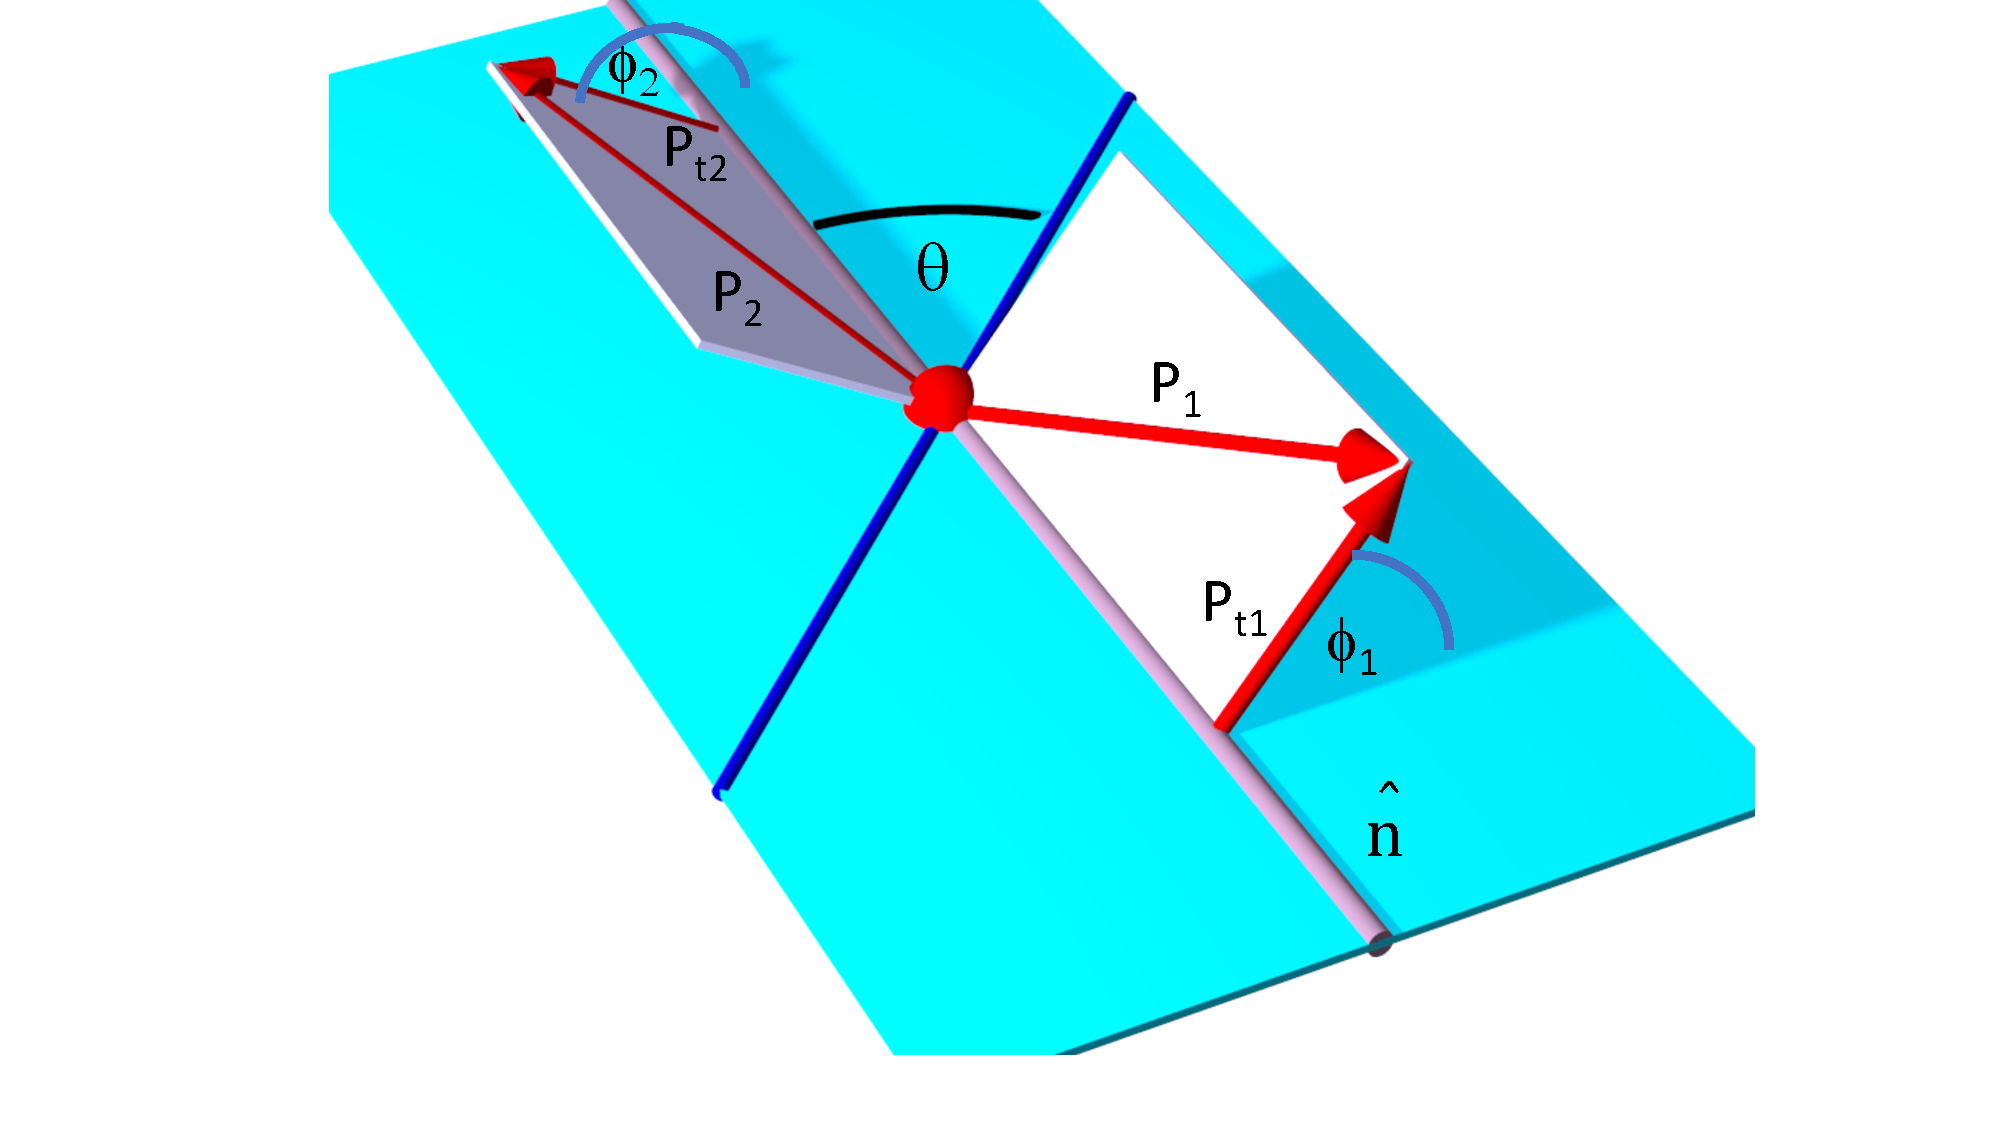
\includegraphics[width=0.8\textwidth]{Collins_angle2.pdf}
\caption{Coordinate system used for this measurement.\label{fig:coo}. See text for details.}
\end{figure}
%%%from note:


% 


%Collins Fragmentation Function appears in the first order transverse moment as~\cite{AsyInPolarizedHadronProductionInEE}:
%\begin{equation}
%H_1^{\bot(1)}=z^2\int d^2 \boldsymbol{k}_T \frac{\boldsymbol{k}_T^2}{2M^2} H_1^{\bot}(z,z^2\boldsymbol{k}_T^2)
%\label{eqn:firstmomet}
%\end{equation}
%\noindent where $H^{\bot q}_1(z,P^2_{h\bot})$ is the Collins FF. Similarly with subsection~\ref{sec:SIDIScrosssubsection}, $z$ is defined as the fractional energy of the hadron $z\approx -\frac{2P_h\cdot q}{Q^2}=\frac{2*E_h}{\sqrt{S}}$. 
%The last item in Eq.~\eqref{eqn:FF1} is dependent on the quark spin direction and hence the transverse distribution function will lead to an asymmetric azimuthal angle distribution as shown in Eq.~\eqref{eqn:tssa}.   


In the following the Collins angle of a hadron pair is defined as $\phi_{12} \equiv \phi_1+\phi_2$. In terms of $\phi_{12}$, the hadron-yield for a given kinematic bin is given by $N_{12}=N_{12}(\phi_{12})$. The normalized rate is computed from $N_{12}$ by dividing by the average yield: $R_{12}(\phi_{12})=\nicefrac{N_{12}}{\langle  N_{12}\rangle}$. Considering the $\cos(\phi_{12})$ modulation, $R_{12}$ can be parameterized as $R_{12}=a_{12}(\theta,z_1,z_2, \boldsymbol{P}^2_{t1},\boldsymbol{P}^2_{t2})\cos(\phi_{12})+b_{12}$ with the azimuthal asymmetry\footnote{The parameters of fits to single ratios are denoted with small letters while capital letters are used for the parametrization of the later-introduced double ratios.}
\begin{equation}
a_{12}(\theta,z_1,z_2, \boldsymbol{P}^2_{t1},\boldsymbol{P}^2_{t2})=\frac{\sin^2\theta}{1+\cos^2\theta}
\frac{\sum\limits_{q}e^2_qH^{\bot q}_1(z_1,\boldsymbol{P}^2_{1\perp})\otimes \bar{H}^{\bot q}_1(z_2,\boldsymbol{P}^2_{2\perp})}{\sum\limits_{q}e^2_qD^q_1(z_1,\boldsymbol{P}^2_{1\perp})\otimes \bar{D}^{\bar{q}}_1(z_2,\boldsymbol{P}^2_{2\perp})}.
\end{equation} 
The $b_{12}$ in the parametrization is the normalized yield, which should be consistent with unity.
Note that in the expression for $a_{12}$ above,  the full dependence of the asymmetry $a_{12}$ on the $z_i$ and $ \boldsymbol{P}^2_{ti}$ is kept. In the measurements presented later in this work,  at most two variables are kept differential, the other ones are integrated over.

Azimuthal distributions can be strongly distorted due to acceptance effects. To remedy those effects the double ratio (DR) method, in which the ratio of normalized distributions from different kinds of hadron pairs is calculated, can be used as the effects are assumed to be charge independent and thus largely cancel in double ratios~\cite{ChargedPionResult,CollinsInSIDISandEE}. In the previous charged pion analysis, one double ratio was defined as the ratio of unlike-sign  ($\pi^+\pi^-$) to like-sign pairs ($\pi^+\pi^+$ and $\pi^-\pi^-$).
Here those are extended to include neutral mesons with the double ratios
\begin{equation}
\label{eqn:FF6}
\begin{aligned}
R_{12}^{\pi^0}=\frac{R^{0\pm}_{12}}{R^L_{12}}&=\frac{\pi^0\pi^++\pi^0\pi^-}{\pi^+\pi^++\pi^-\pi^-}\\
R_{12}^{\eta}=\frac{R^{\eta\pm}_{12}}{R^L_{12}}&=\frac{\eta\pi^++\eta\pi^-}{\pi^+\pi^++\pi^-\pi^-}.
\end{aligned}
\end{equation}
For charged pions asymmetries of like-sign pairs (L), unlike-sign pairs (U), or pairs that are summed over both charges (C) can be considered.
With these the following three double ratios can be constructed:
%
\begin{equation}
\label{eqn:FF7}
\begin{aligned}
R_{12}^{UL}=\frac{R^{U}_{12}}{R^L_{12}}&=\frac{\pi^+\pi^-+\pi^-\pi^+}{\pi^+\pi^++\pi^-\pi^-}\\
R_{12}^{UC}=\frac{R^{U}_{12}}{R^C_{12}}&=\frac{\pi^+\pi^-+\pi^-\pi^+}{\pi^+\pi^++\pi^-\pi^-+\pi^+\pi^-+\pi^-\pi^+}\\
R_{12}^{CL}=\frac{R^{C}_{12}}{R^L_{12}}&=\frac{\pi^+\pi^++\pi^-\pi^-+\pi^+\pi^-+\pi^-\pi^+}{\pi^+\pi^++\pi^-\pi^-}.
\end{aligned}
\end{equation}
%
The double ratio $R^C$ is thought to be related to those involving $\pi^0$s, therefore the double ratio $R_{12}^{CL}$ should be consistent with $R_{12}^{\pi^0}$~\cite{Efremov:2006qm}.
%We will test with the experimental data.
%For the Collins effect, the Collins FF can be separated into favored and unfavored parts according to which flavor goes into the hadron where charge-conjugation and isospin symmetry arguments have been used~\cite{CollinsInSIDISandEE}:


Fragmentation functions are often categorized into favored and disfavored ones, depending on whether or not the fragmenting-quark flavor is part of the valence structure of the hadron formed. For charged pions, employing charge-symmetry and isospin asymmetry, the non-strange FFs are 
\begin{equation}
\begin{aligned}
D^{fav}&=D^{u/{\pi^+}}=D^{d/{\pi^-}}=D^{\bar{u}/{\pi^-}}=D^{\bar{d}/{\pi^+}}\\
D^{dis}&=D^{u/{\pi^-}}=D^{d/{\pi^+}}=D^{\bar{u}/{\pi^+}}=D^{\bar{d}/{\pi^-}}.
\label{eqn:FF4}
\end{aligned}
\end{equation}
The fragmentation functions for $\pi^0$ consist of both favored and disfavored FFs~\cite{FoundationsofpQCD,Efremov:2006qm},
\begin{equation}
\begin{aligned}
D^{u/{\pi^0}}=D^{\bar{u}/{\pi^0}}=D^{d/{\pi^0}}=D^{\bar{d}/{\pi^0}}=\frac{1}{2}(D^{dis}+D^{fav}).
\label{eqn:FF4pi0}
\end{aligned}
\end{equation}
Besides light quarks, the contribution of strange quarks is also considered.
% A common assumption is that the probability for strange-quark fragments into charged pions is the same as the light-quark disfavored ones, as it also requires generating the two valence quarks forming the pion, thus
A common assumption is that the probability for strange-quark fragmentation is the same for all pion states, thus
\begin{equation}
D^{dis}_{s\rightarrow\pi}=D^{s/{\pi^-}}=D^{s/{\pi^+}}=D^{s/{\pi^0}}=D^{\bar{s}/{\pi^-}}=D^{\bar{s}/{\pi^+}}=D^{\bar{s}/{\pi^0}}.
\end{equation}
%
Similarly, the FFs for $\eta$ production can be simplified to 
%
\begin{equation}
\begin{aligned}
D^{u/{\eta}}&=D^{d/{\eta}}=D^{\bar{u}/{\eta}}=D^{\bar{d}/{\eta}}=\frac{1}{2}\left(D^{fav_\eta}+D^{dis_\eta}\right) \\
D^{s/{\eta}}&=D^{\bar{s}/{\eta}}
\label{eqn:FFetaquark}
\end{aligned}
\end{equation}

 
The various double ratios, e.g., of $\pi^0\pi^{\pm}$ pairs ($R^{0\pm}_{12}$) and like-sign pairs ($R^L_{12}$), can then be expressed in terms of these FFs~\cite{Efremov:2006qm}:

\begin{multline}
R_{12}^{\pi^0}=\frac{R^{0\pm}_{12}}{R^L_{12}}=1+\cos(\phi_1+\phi_2)\frac{\sin^2(\theta)}{1+\cos^2(\theta)} \\
\times\bigg\{\frac{5(H^{\bot,fav}_1+H^{\bot,dis}_1)(H^{\bot,dis}_1+H^{\bot,fav}_1)+4H^{\bot,dis}_{1,s\rightarrow\pi}H^{\bot,dis}_{1,s\rightarrow\pi}}{5(D^{fav}_1+D^{dis}_1)(D^{dis}_1+D^{fav}_1)+4D^{dis}_{1,s\rightarrow\pi}D^{dis}_{1,s\rightarrow\pi})}\\
-\frac{5H^{\bot,fav}_1H^{\bot,dis}_1+5H^{\bot,dis}_1H^{\bot,fav}_1+2H^{\bot,dis}_{1,s\rightarrow\pi}H^{\bot,dis}_{1,s\rightarrow\pi}}{5D^{fav}_1D^{dis}_1+5D^{dis}_1D^{fav}_1+2D^{dis}_{1,s\rightarrow\pi}D^{dis}_{1,s\rightarrow\pi}} \bigg\}.
\label{eqn:FF5}
\end{multline}




%Due to the differing valence structure of the $\eta$, the FFs composition the relations above~\ref{eqn:FF5} read differently:


%Neglecting symmetry breaking due to strangeness suppression, the strange-quark FFs can be related to the non-strange ones:
%\begin{equation}
%\begin{aligned}
%D^{s/{\eta}}=D^{\bar{s}/{\eta}}=\frac{1}{2}\left(D^{fav_\eta}+D^{dis_\eta}\right).`
%\end{aligned}
%\end{equation}
%However, here we do not use this relation. 
Using Eq.~\eqref{eqn:FFetaquark} results in the following expression for the \(\eta\) double ratio:
\begin{multline}
R_{12}^{\eta}=\frac{R^{\eta\pm}_{12}}{R^L_{12}}=1+\cos(\phi_1+\phi_2)\frac{\sin^2(\theta)}{1+\cos^2(\theta)} \\
\times\bigg\{\frac{5(H^{\bot,fav_\eta}_1+H^{\bot,dis_\eta}_1)(H^{\bot,dis}_1+H^{\bot,fav}_1)+2(H^{\bot,fav}_{1,s\rightarrow\eta}+H^{\bot,dis}_{1,s\rightarrow\eta})H^{\bot,dis}_{1,s\rightarrow\pi}}{5(D^{\bot,fav_\eta}_1+D^{\bot,dis_\eta}_1)(D^{\bot,dis}_1+D^{\bot,fav}_1)+2(D^{dis}_{1,s\rightarrow\eta}+D^{dis}_{1,s\rightarrow\eta})D^{dis}_{1,s\rightarrow\pi})}\\
-\frac{5H^{\bot,fav}_1H^{\bot,dis}_1+5H^{\bot,dis}_1H^{\bot,fav}_1+2H^{\bot,dis}_{1,s\rightarrow\pi}H^{\bot,dis}_{1,s\rightarrow\pi}}{5D^{\bot,fav}_1D^{\bot,dis}_1+5D^{\bot,dis}_1D^{\bot,fav}_1+2D^{dis}_{1,s\rightarrow\pi}D^{dis}_{1,s\rightarrow\pi}} \bigg\}.
\label{eqn:FF5eta}
\end{multline}
The charged pion double ratios $R^{UL}_{12}$ and $R^{UC}_{12}$ can be written in terms of the various fragmentation functions as
%
\begin{equation}
\begin{aligned}
R^{UL}_{12}&=1+\cos(\phi_1+\phi_2)\frac{\sin^2(\theta)}{1+\cos^2(\theta)}\\
&\times\bigg\{\frac{5(H^{\bot,fav}_1H^{\bot,fav}_1+H^{\bot,dis}_1H^{\bot,dis}_1)+2H^{\bot,dis}_{1,s\rightarrow\pi}H^{\bot,dis}_{1,s\rightarrow\pi}}{5(D^{fav}_1D^{fav}_1+D^{dis}_1 D^{dis}_1)+2D^{dis}_{1,s\rightarrow\pi}D^{dis}_{1,s\rightarrow\pi}}\\
&-\frac{5H^{\bot,fav}_1 H^{\bot,dis}_1+H^{\bot,dis}_{1,s\rightarrow\pi}H^{\bot,dis}_{1,s\rightarrow\pi}}{5D^{fav}_1D^{dis}_1 +D^{dis}_{1,s\rightarrow\pi}D^{dis}_{1,s\rightarrow\pi}} \bigg\} 
\end{aligned}
\label{eqn:allratiosexpress2}
\end{equation}
\begin{equation}
\begin{aligned}
R^{UC}_{12}&=1+\cos(\phi_1+\phi_2)\frac{\sin^2(\theta)}{1+\cos^2(\theta)}\\
&\times\bigg\{\frac{5(H^{\bot,fav}_1H^{\bot,fav}_1+H^{\bot,dis}_1H^{\bot,dis}_1)+2H^{\bot,dis}_{1,s\rightarrow\pi}H^{\bot,dis}_{1,s\rightarrow\pi}}{5(D^{fav}_1D^{fav}_1+D^{dis}_1D^{dis}_1)+2D^{dis}_{1,s\rightarrow\pi}D^{dis}_{1,s\rightarrow\pi}}\\
&-\frac{5(H^{\bot,fav}_1+H^{\bot,dis}_1)(H^{\bot,dis}_1+H^{\bot,fav}_1)+4H^{\bot,dis}_{1,s\rightarrow\pi}H^{\bot,dis}_{1,s\rightarrow\pi}}{5(D^{fav}_1+D^{dis}_1)(D^{dis}_1+D^{fav}_1)+4D^{dis}_{1,s\rightarrow\pi}D^{dis}_{1,s\rightarrow\pi}} \bigg\}
\end{aligned}
\label{eqn:allratiosexpress3}
\end{equation}
The parameterization $A_{12} \cos(\phi_1+\phi_2)$ is fitted to the final double-ratio azimuthal distribution, where the amplitude $A_{12}$ is the azimuthal asymmetry that is measured in this work for various meson combinations. 

%%%%%%%%%%%%%
%%%%%%%%%%%%from note
%%%%%%%%%%%%



\section{Experiment}
The Belle experiment~\cite{BelleDetector} at the KEKB storage ring~\cite{KEKB} recorded about 1~ab$^{-1}$ of $e^+e^-$ annihilation data. The data was taken mainly at the $\Upsilon(4S)$ resonance at $\sqrt{s}=10.58$~GeV, but also at $\Upsilon(1S)$ to $\Upsilon(5S)$ resonances and at $\sqrt{s}=10.52$~GeV.
%but roughly 10\% of it was taken just below this energy at $\sqrt{s}=10.52$~GeV.
The Belle instrumentation used in this analysis includes a central drift chamber and a silicon vertex detector, which provides precision tracking for tracks in $17.0\degree < \theta_\textrm{Lab}< 150.0\degree$, 
and electromagnetic calorimeters (ECL) covering the same region. % The ECL is subdivided into a barrel region ($0.56~\textrm{rad} < \theta_\textrm{Lab} < 2.25~\textrm{rad}$) and the endcaps. 
Particle identification is performed using information on dE/dx in the CDC, a time-of-flight system in the barrel, aerogel Cherenkov counters in the barrel and the forward endcap, as well as a muon and $K_L$ identification system outside the superconducting solenoid, which provides a 1.5~T magnetic field.
\label{sec:experiment}
\section{Analysis}
\label{sec:analysis}

Similar to previous work~\cite{Abe:2005zx,Seidl:2008xc, Vossen:2011fk}, hadronic events are selected by requiring a minimum visible energy of 7~GeV and a thrust $t > 0.8$. 
These cuts reduce the contribution of $\tau$ leptons and $B$ mesons to below 1\% and allows the inclusion of all on- and off-resonance data in the analysis.
A number of fiducial cuts are applied with the goal to minimize effects from variations of the acceptance functions of the detector on the extracted asymmetries.
For this reason only mesons reconstructed from tracks and photons in the barrel region of the detector are considered. Table~\ref{tab:cuts} lists the fiducial as well as the other cuts applied.
\begin{table}
\begin{tabular}{ll}
Description & cut value\\
\hline
Minimum visible energy $E_\textrm{vis}$ cut &$E_\textrm{vis}>7$~GeV\\
Thrust cut & $t>0.8$\\
Opening angle $\alpha_O$ of reconstructed meson \em{w.r.t.} $\boldsymbol{\hat{n}}$\qquad \phantom{f} & $\alpha_O< 0.3$\\
Thrust axis polar angle $\theta_{\boldsymbol{\hat{n}}}$&$1.34< \theta_{\boldsymbol{\hat{n}}}<2.03$\\
min photon energy $E_{\gamma,\pi^0}$ cut for $\pi^0$ &$E_{\gamma,\pi^0}>50$~MeV \\
min photon energy cut $E_{\gamma,\eta}$  for $\eta$ &$E_{\gamma,\eta}>150$~MeV \\
Opening angle $\alpha_{O,\gamma}$ for photons \em{w.r.t.} $\boldsymbol{\hat{n}}$&$\alpha_{O,\gamma}<0.5$\\



\end{tabular}
\caption{Cuts applied in the analysis. See text for description.\label{tab:cuts}}
\end{table}

To minimize the impact of the fiducial cuts on the extracted asymmetry, a hierarchical set of opening angle cuts on photons, hadron momenta and the thrust axis is applied. This ensures that the acceptance of all mesons is radially symmetric around the thrust axis and the acceptance in $z$ and $P_t$ of charged and neutral mesons is approximately equal. All photons used for the reconstruction of $\pi^0$ and $\eta$ mesons have a maximal opening angle of 0.5 from the thrust axis in the CMS. All charged and reconstructed neutral mesons used in the asymmetry computation are required to have a maximal opening angle of 0.3 from the thrust axis in the CMS. Finally, the thrust axis polar angle is restricted to $1.34< \theta_{\boldsymbol{\hat{n}}} < 2.03$ in the CMS to ensure the radial symmetry of the acceptance for photons inside the barrel around the thrust axis. 
To reconstruct $\pi^0$ and $\eta$ mesons, pairs of photons are used for which a minimum energy cut of 50~MeV and 150~MeV, respectively, is imposed to reduced background.  The signal is extracted using a crystal-ball fit~\cite{CrystalBallFunc} in the signal region and a $5^\textrm{th}$ order polynomial for the background. Some exemplary fits for $\pi^0$ and $\eta$ mesons are shown in Fig.~\ref{fig:crystalfit}. The agreement of the extracted signal with simulations was verified. 
The simulations used in this analysis uses Pythia~\cite{Sjostrand:2006za} and EvtGen~\cite{Lange:2001uf} for various physics processes not including the polarization dependent Collins effect, and GEANT3~\cite{Brun:1987ma} for the detector effects.  
For low $z$ bins some disagreement between the extracted $\pi^0$ signal from experimental data and simulation was observed. Therefore an (almost) non-parametric method, that does not rely on the fit of the signal, was used as well. For this, the background was extracted from the sideband region, where data and simulation agree well, using simulation data. The background in this case is defined as any pair of electromagnetic clusters that do not come from the same $\pi^0$.
Then the background in the signal region is estimated using a quadratic fit to 20 points in the upper and lower sidebands, respectively and the signal is extracted as the difference between the estimated background and the observed yield in the signal region. The difference between the two extraction methods for the final asymmetry is small, typically less than one per-mille in absolute asymmetry value, and is added to final systematic uncertainties.

The charged pion selection relies on the Belle PID in the barrel and achieves a purity of 97\% over all kinematic bins.
The thrust axis is reconstructed from all charged tracks, using the available PID information, and photons.




\begin{figure}
  \centering     
  \subfigure[$\pi^0$ invariant mass fit, $0.2<z<0.3$]{\label{fig:pi0crystalfit_1}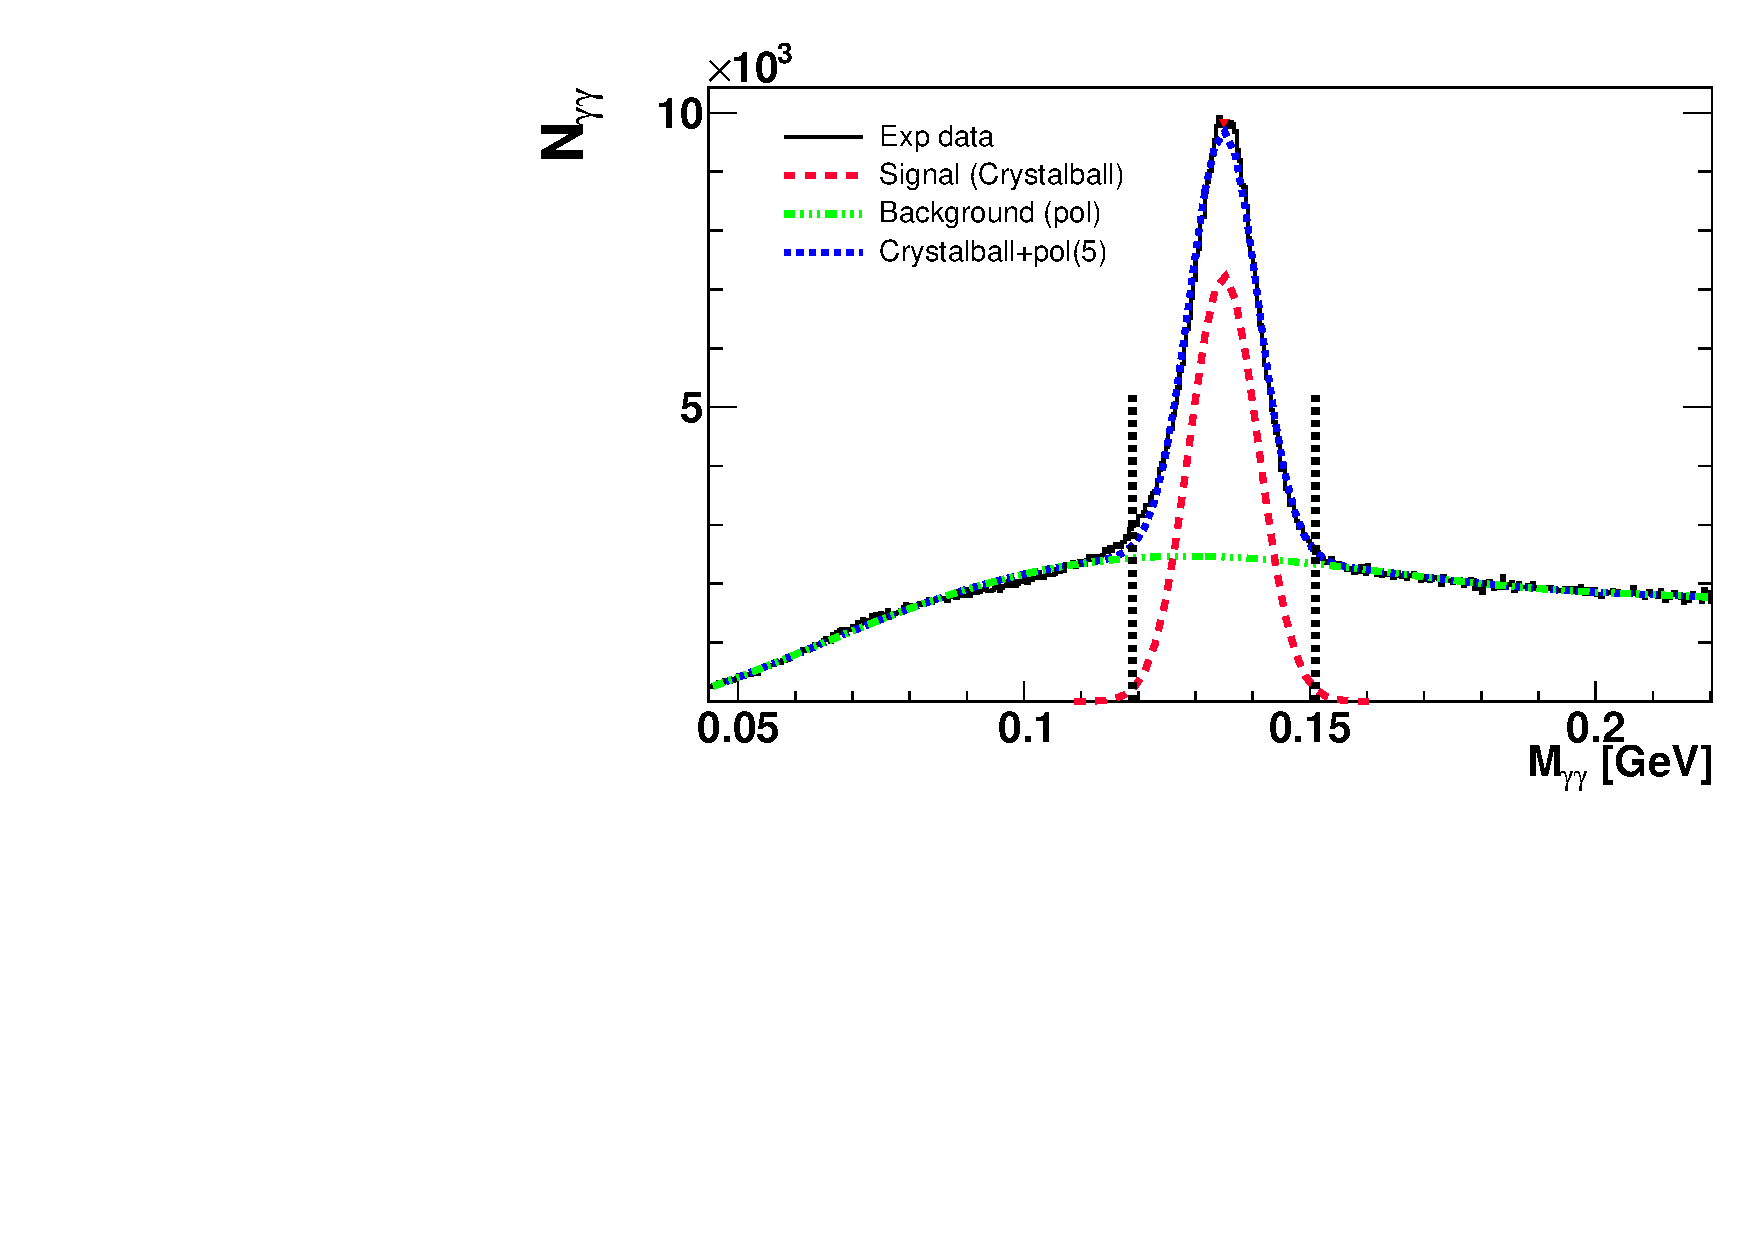
\includegraphics[width=.48\textwidth]{pi0_crystalfit_Z_1.pdf}}
  \subfigure[$\pi^0$ invariant mass fit, $0.6<z<0.7$]{\label{fig:pi0crystalfit_2}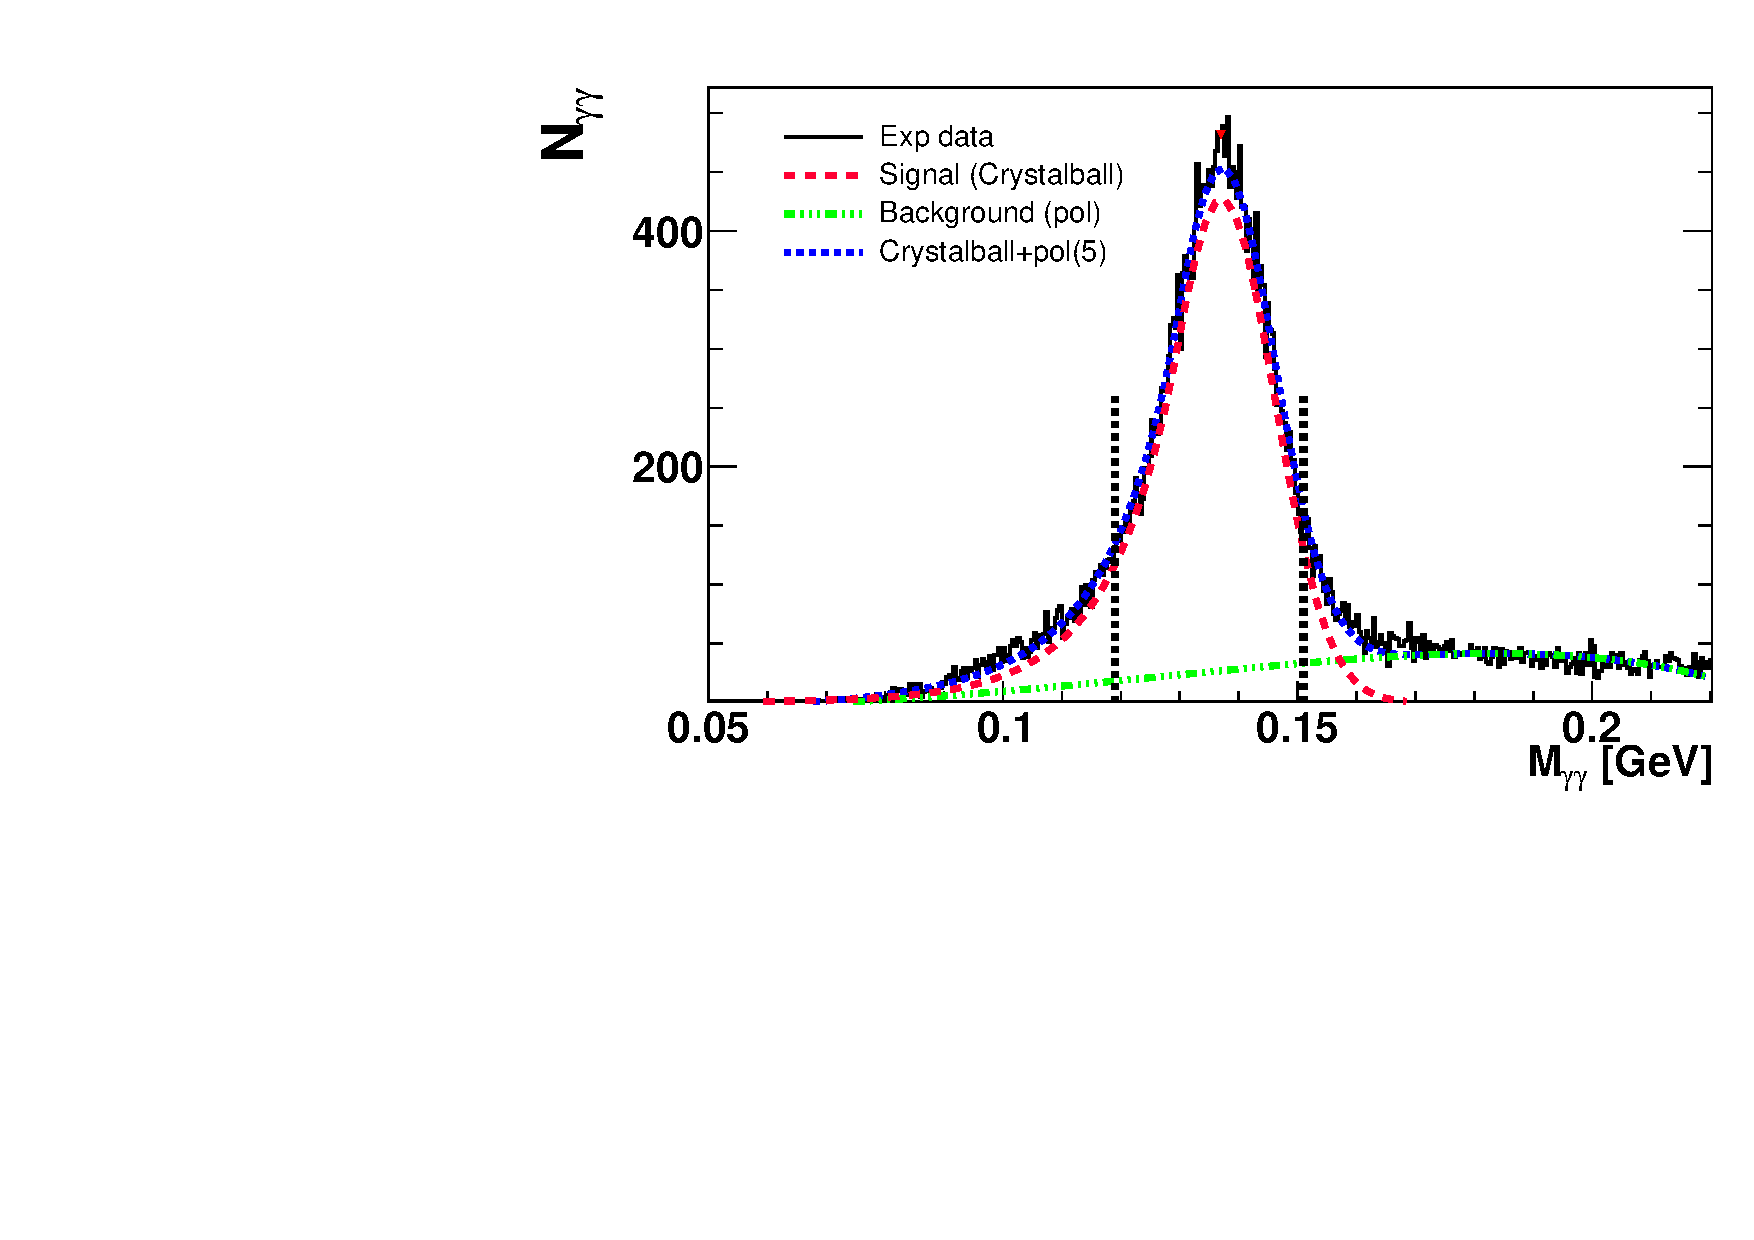
\includegraphics[width=.48\textwidth]{pi0_crystalfit_Z_5.pdf}}
    \subfigure[$\eta$ invariant mass fit, $0.3<z<0.4$]{\label{fig:etacrystalfit_1}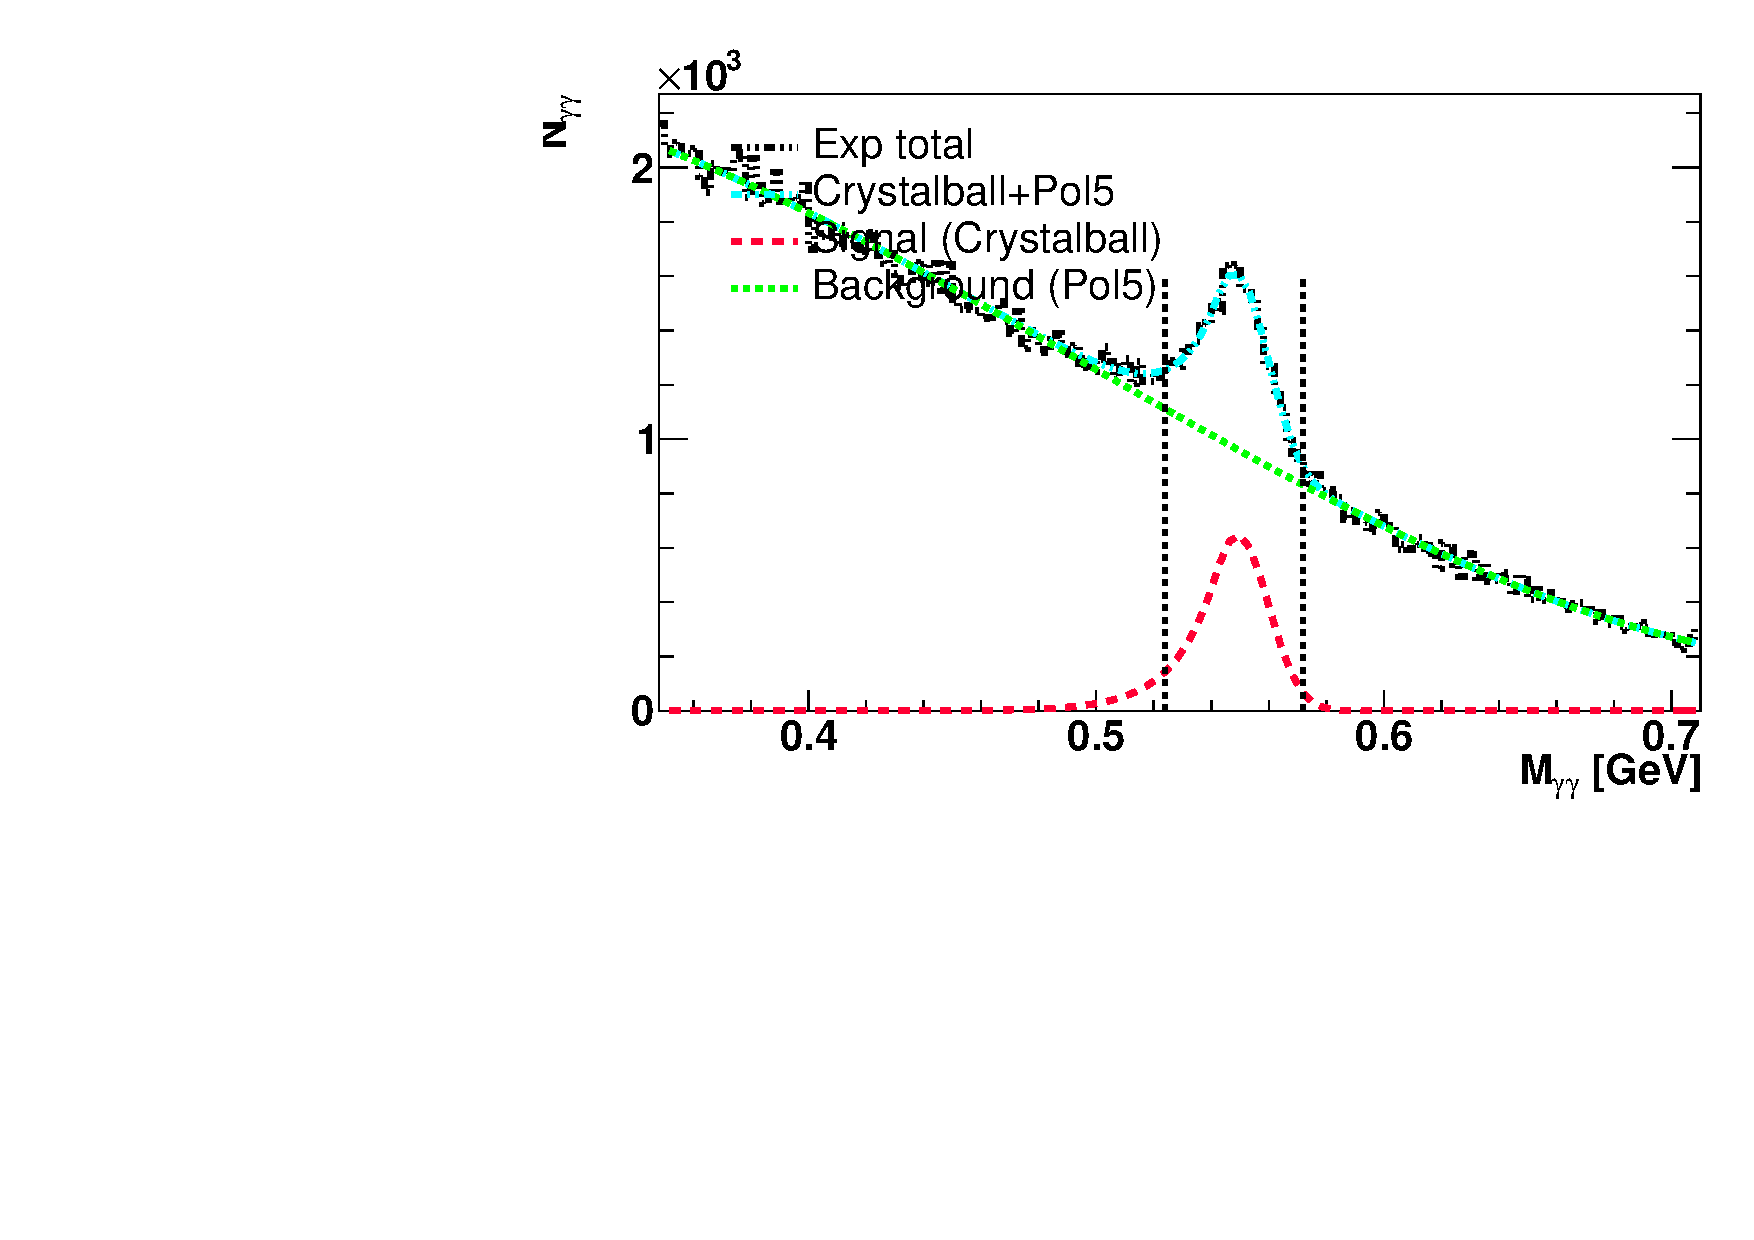
\includegraphics[width=.48\textwidth]{eta_fitall_Z_2.pdf}}
  \subfigure[$\eta$ invariant mass fit, $0.6<z<0.7$]{\label{fig:etacrystalfit_2}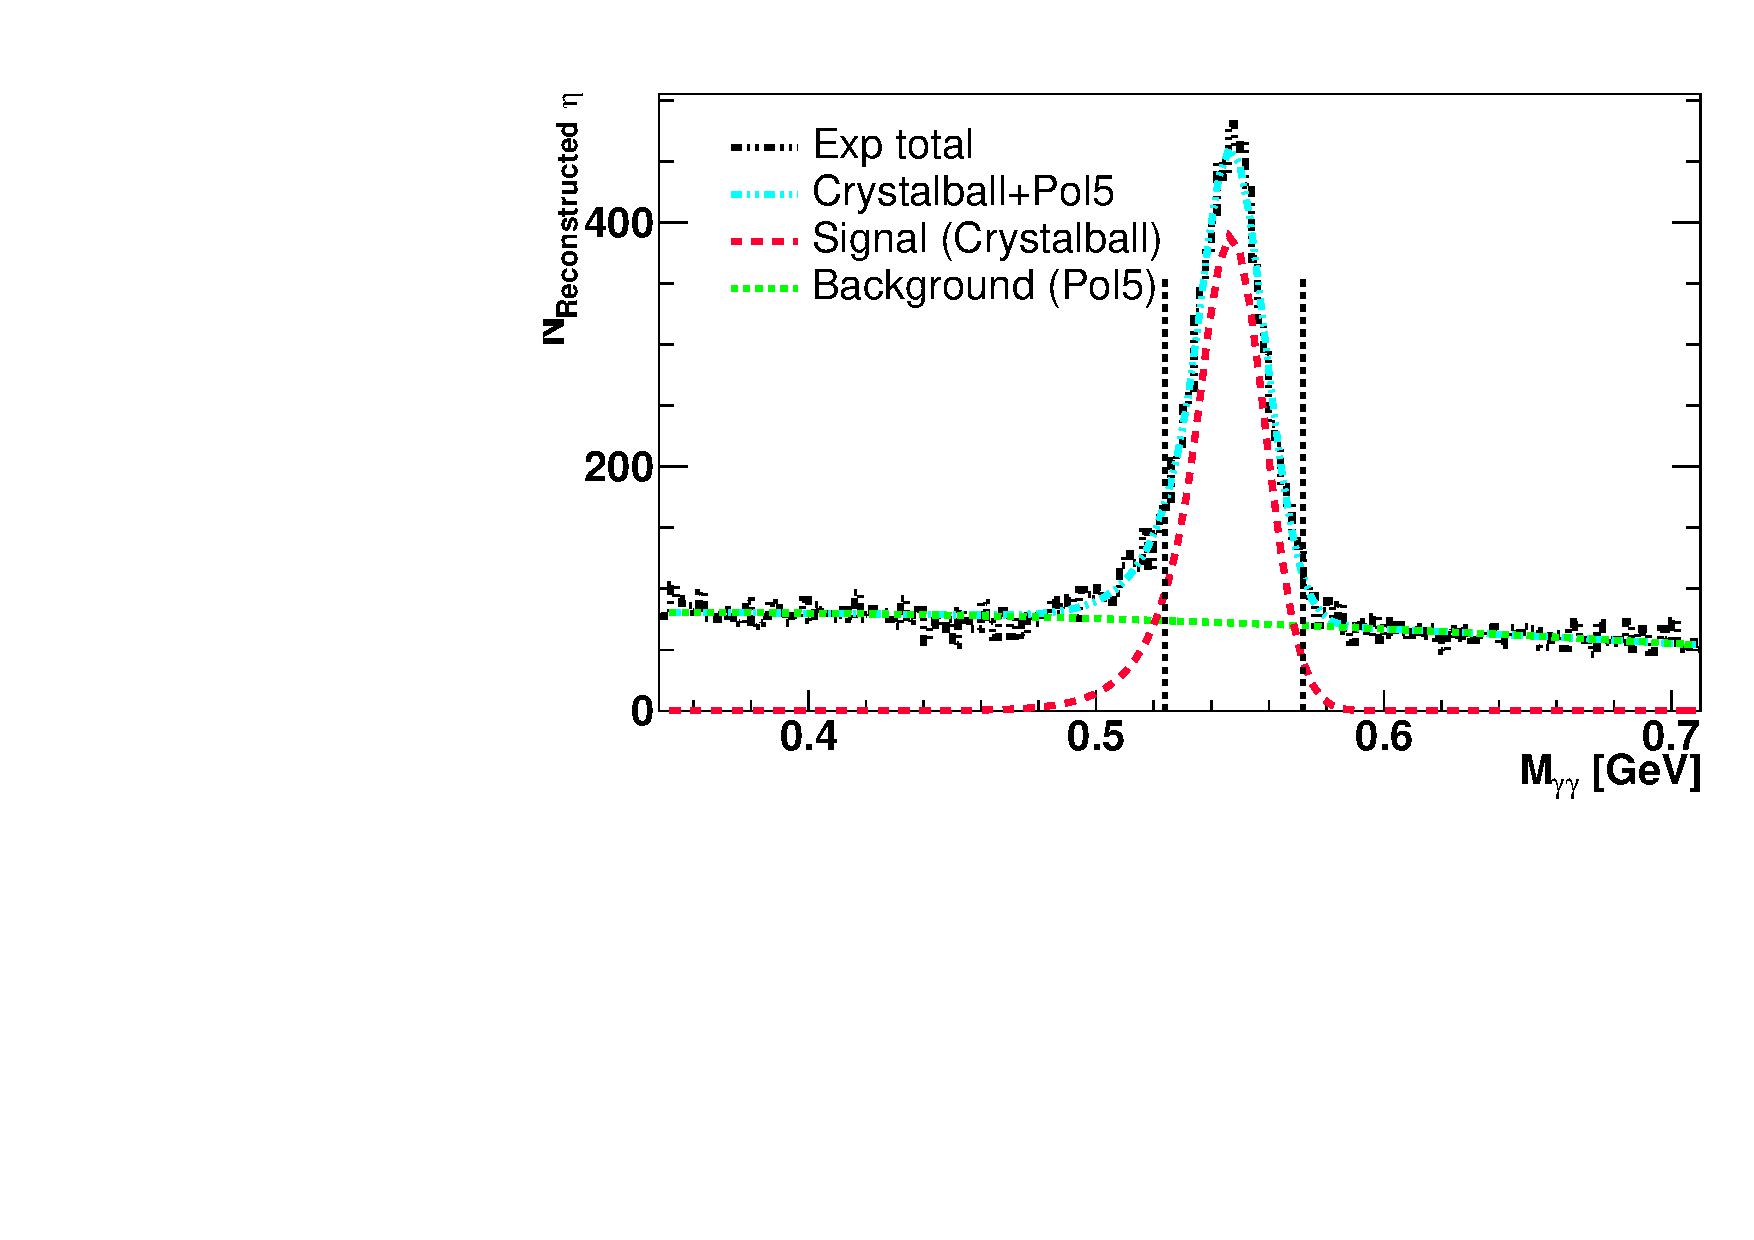
\includegraphics[width=.48\textwidth]{eta_fitall_Z_5.pdf}}
  \caption{Typical two-photon invariant mass distributions with fit using a Crystal Ball function for the signal and a polynomial background function for $\pi^0$ (top plots) and $\eta$ (bottom plot) mesons. In each plot, the green line represents the fitted background using a polynomial of 5th order, the red line the fitted signal and the blue line is the combined background and signal fit. It agrees well with the experimental data in black. The vertical dash lines are the boundaries of the signal region.}
  \label{fig:crystalfit}
\end{figure}


Using the thrust axis $\boldsymbol{\hat{n}}$, and the reconstructed meson momenta, the azimuthal angles $\phi_1$ and $\phi_2$ for back-to-back pairs of mesons are computed using Eq.~\ref{eqn:collinsangledefine2}.



%\begin{equation}
%\phi_{i}=\textrm{sgn}\left(\boldsymbol{\hat{n}}\cdot\left((\boldsymbol{e}\times \boldsymbol{\hat{n}})\times(\boldsymbol{\hat{n}}\times\boldsymbol{P_i}) \right) \right) \arccos\left( \frac{\boldsymbol{e}\times \boldsymbol{\hat{n}}}{|\boldsymbol{e}\times\boldsymbol{\hat{n}}|} \cdot \frac{\boldsymbol{\hat{n}} \times \boldsymbol{P_i}}{|\boldsymbol{\hat{n}}\times\boldsymbol{P_i}|}  \right).
%\label{eq:phi12}
%\end{equation}


Finally, the ratios of $\cos(\phi_1+\phi_2)$ dependent yields in Eqs.~\eqref{eqn:FF5}-\eqref{eqn:allratiosexpress3} are constructed and fitted to extract raw asymmetries binned in $z_i$ and $P_{ti}$. Here the first index is always referring to the neutral meson in the pair. For the pairs of charged hadrons, the assignment of the first and second hadron in a pair is random. The binning in $z$ and $P_t$ reflects the dependency of the fragmentation functions that are to be extracted from this data.
To determine the final asymmetries, corrections are applied to the raw asymmetries. First, the raw asymmetries are corrected for the contribution of the background. For this, the asymmetry is measured in the upper and lower sidebands as well as the signal region. The asymmetry in the signal region is corrected based on the signal to background ratios in these three regions as well as a linear extrapolation of the background asymmetry under the signal peak. 	
Then, the so-called false asymmetries, determined from simulations, is subtracted. Since the simulation does not contain the Collins effect, any residual signal is due to acceptance effects. They are consistent with zero within their statistical uncertainties and  those uncertainties are added to our final systematic uncertainties. The relative contribution of these uncertainties ranges from the sub-percent level at low $z$ to a few percent at high $z$.


Finally, the  asymmetries are corrected for thrust smearing and bin migration effects. The effect on the reconstructed $z$ values is negligible, while it has a significant impact on the reconstructed $P_t$. A weighted simulation that reproduces the observed kinematical dependence of the real data is produced by using a weighted asymmetry with $P_ {t1},P_{t2}$ dependent magnitude of the form $1+a_{N,D}P_{t1}P_{t2}$. Here $a$ is a factor that is chosen independently for nominator ($a_N$) and denominator ($a_D$) of the double ratios in each $z$ bin to reproduce the measured asymmetries. Using this weighted simulation, a correction factor $f_S$ for each bin is calculated. The factors $a_N$ and $a_D$ an be determined with the exception of a common scaling factor. The dependence of the smearing factor on this scaling factor and on reasonable variations of the ratio $\nicefrac{a_N}{a_D}$ was observed to be negligible. 
This factor is calculated as the ratio of the input asymmetries, using the true thrust axis and the true kinematics of the detected hadrons, and the reconstructed asymmetries. The uncertainties on $f_S$ are also added to the final systematic uncertainty. Values for $f_S$ are between $f_S=1.2$ and $f_S=1.3$ with the exception of the kinematic boundaries in the lowest $P_t$ bin or when both particles in the pair are in the highest $z$ bin. Here the hadrons are close to the thrust axis, enhancing smearing effects and the correction factor takes values between $f_S=1.4$ and $f_S=1.5$ depending on particle species. The relative uncertainty on $f_S$ is again determined by our Monte-Carlo statistics and is below 2\% in the single $z$ binning, while for the binning in both hadron $z$ values it is below 3\% for most bins, but reaches 10\% for the highest $z_1$,$z_2$ bin. 

%The average value of $f_C$ is $1.25$ and is between $1.2$ and $1.3$ for all $z$ and $P_t$ bins, with the exception of the lowest $P_t$ bin and the case where both hadrons in the pair are in the highest $z$ bin. Here the hadrons are close to the thrust axis, enhancing smearing effects and we get $f_C=1.4$. 

%%%
%%% from note, master formular
%%%
The applied corrections for smearing effects, background contributions, and false asymmetries can be summarized in eq.~\eqref{eq:masterCorrection}:
\begin{equation}
A=(A_\textrm{raw,bg corrected}-A_\textrm{MC})\times f_S\, .
\label{eq:masterCorrection}
\end{equation}
Here, $A_\textrm{raw,bg corrected}$ is the raw asymmetry after background correction.
$A_\textrm{MC}$ is the false asymmetry measured in simulation.
%The later are not corrected for background asymmetries, since we are only interested in the detector effects on the asymmetries.
Finally, the asymmetry is corrected for smearing using the smearing correction $f_S$.
Similarly systematic uncertainties that arise from the statistical uncertainties on the smearing effects, the background contribution and the false asymmetries can be summarized in eq.~\eqref{eq:masterSys}:
\begin{equation}
\sqrt{ A^2*(\frac{\sigma_{f_S}}{f_S})^2+(f_S*\sigma_F)^2+(f_S*\sigma_{A_\textrm{MC}})^2}.
\label{eq:masterSys}
 \end{equation}
 Here $\sigma_F$ is the uncertainty on the fit to extract the $\pi^0$ signal. 
 %As described in Section~\ref{sec:neutralmesonreconstruction}, this uncertainty accounts for the difference in extracted asymmetries if either the crystal-ball fit or the non-parametric signal fit using MC templates is used to determine the signal count rates. The crystal-ball result is used for the actual asymmetry value.
 

\section{Results}
\label{sec:results}
Results shown in this section are binned in $z$ and $P_t$. 
Since smearing effects are largest and the Collins effect is smallest at low $z$, a cut of $z_1>0.2$ is used with the exception of the results which are binned both, in $z_1$ and $z_2$. Bin boundaries above 0.2 are $0.3,0.4, 0.5, 0.6, 0.7,1.0$. For the $\eta$, due to its higher mass, a  cut of $z>0.3$ is used. For the $P_t$ binning, bin boundaries of $0,0.15,0.3,0.5$  and $3$~\nicefrac{GeV}{c} are used. 
Figure~\ref{fig:resPi0VsZ1Z2} shows the result of $A^{\pi^0}_{12}$ versus $z_1$ and $z_2$. As expected from previous results, significant asymmetries with an almost linear dependence on $z$, reaching $20$\% in the highest $z_1,z_2$ bin, are observed. 


\begin{figure}
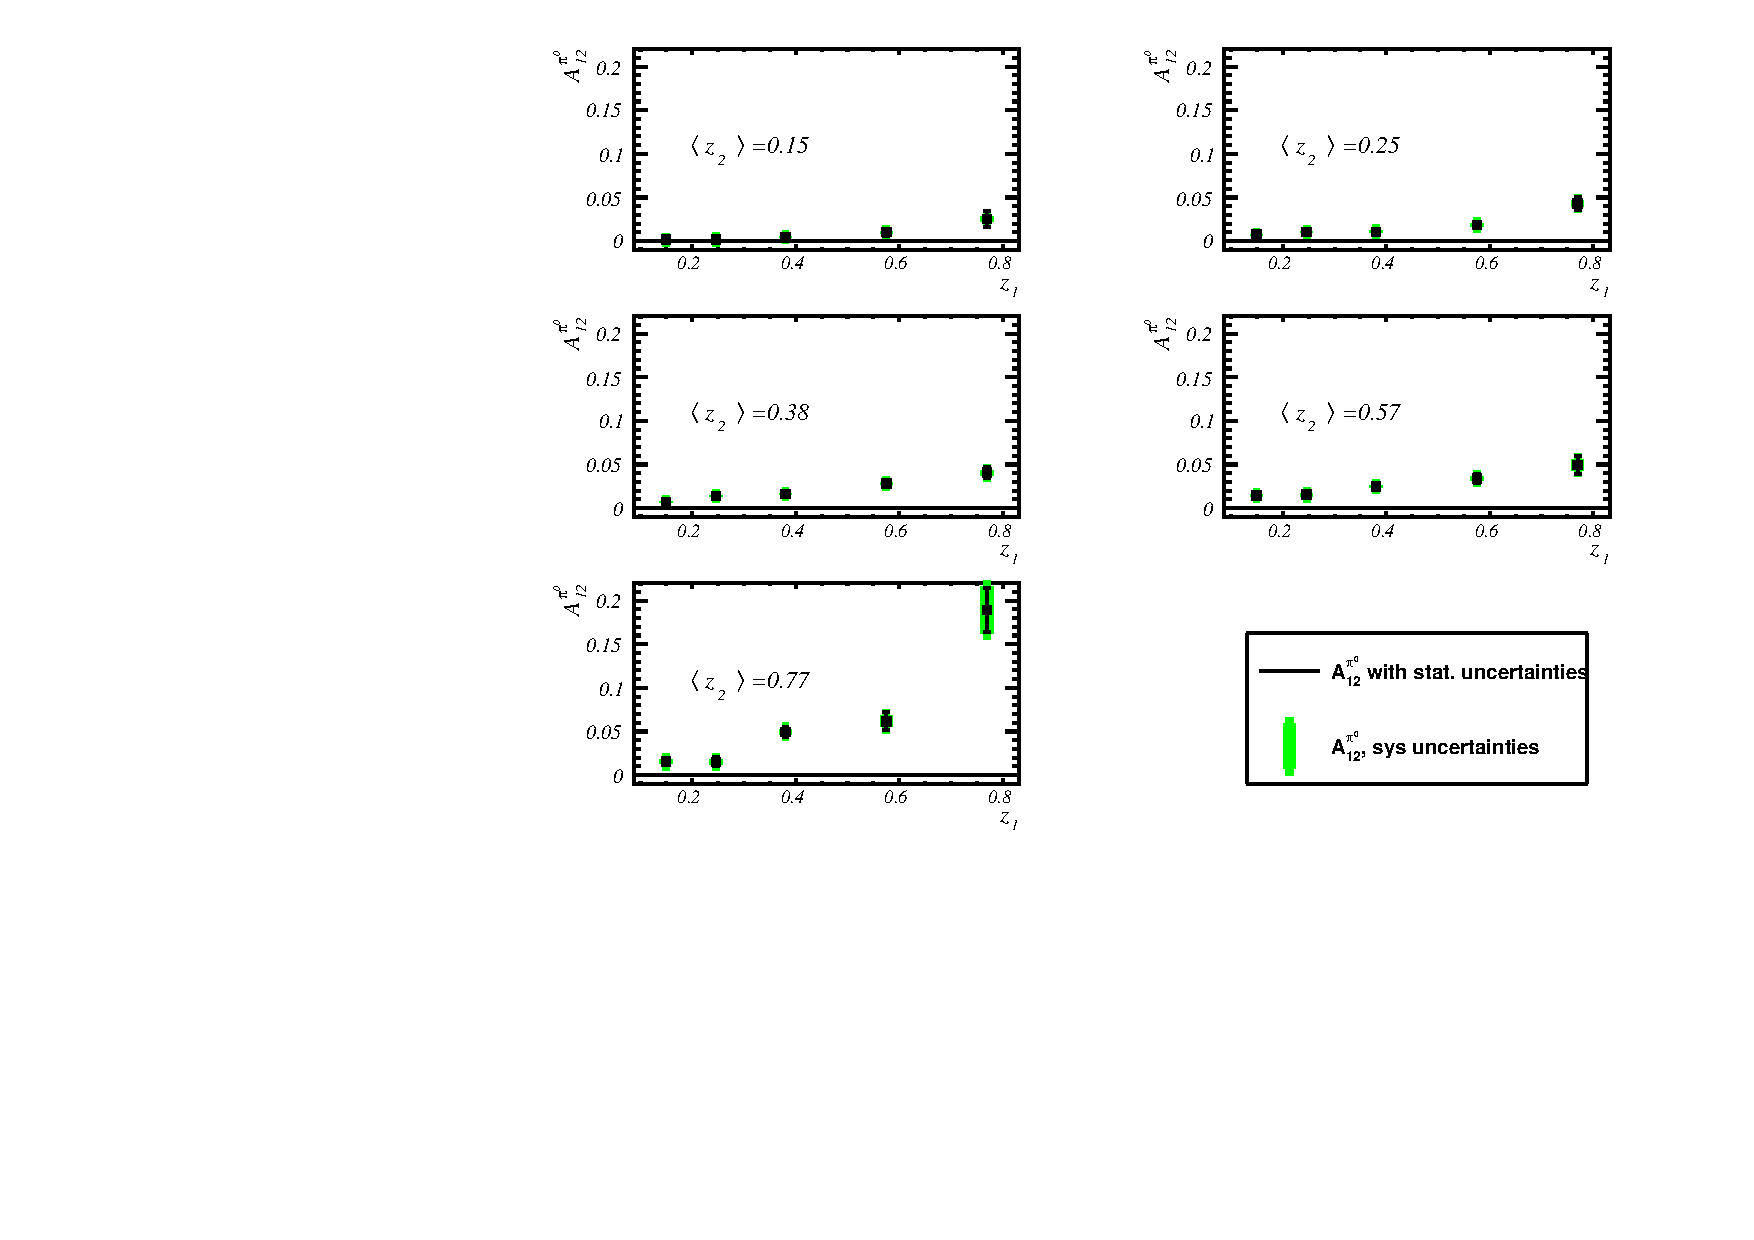
\includegraphics[width=0.95\textwidth]{figs_paper/pi0VsZ1Z2.pdf}
\caption{Results for $A^{\pi^0}_{12}$ vs. $z_1,z_2$. Significant asymmetries are observed, which rise with $z_1$ and $z_2$.\label{fig:resPi0VsZ1Z2}. See discussion in the text.}
\end{figure}

Figure~\ref{fig:resPi0VsZPt} shows the results for $A^{\pi^0}_{12}$ versus $z_1$ and $P_{t1}$. As expected, for $P_{t1}$ approaching zero, the asymmetry vanishes. The dependence on $P_{t1}$ seems almost linear and the $P_t$ reach is not enough to see a plateauing of the asymmetries at high $P_t$. Higher values of $z_1$ are again associated with larger values of $A^{\pi^0}_{12}$.
\begin{figure}
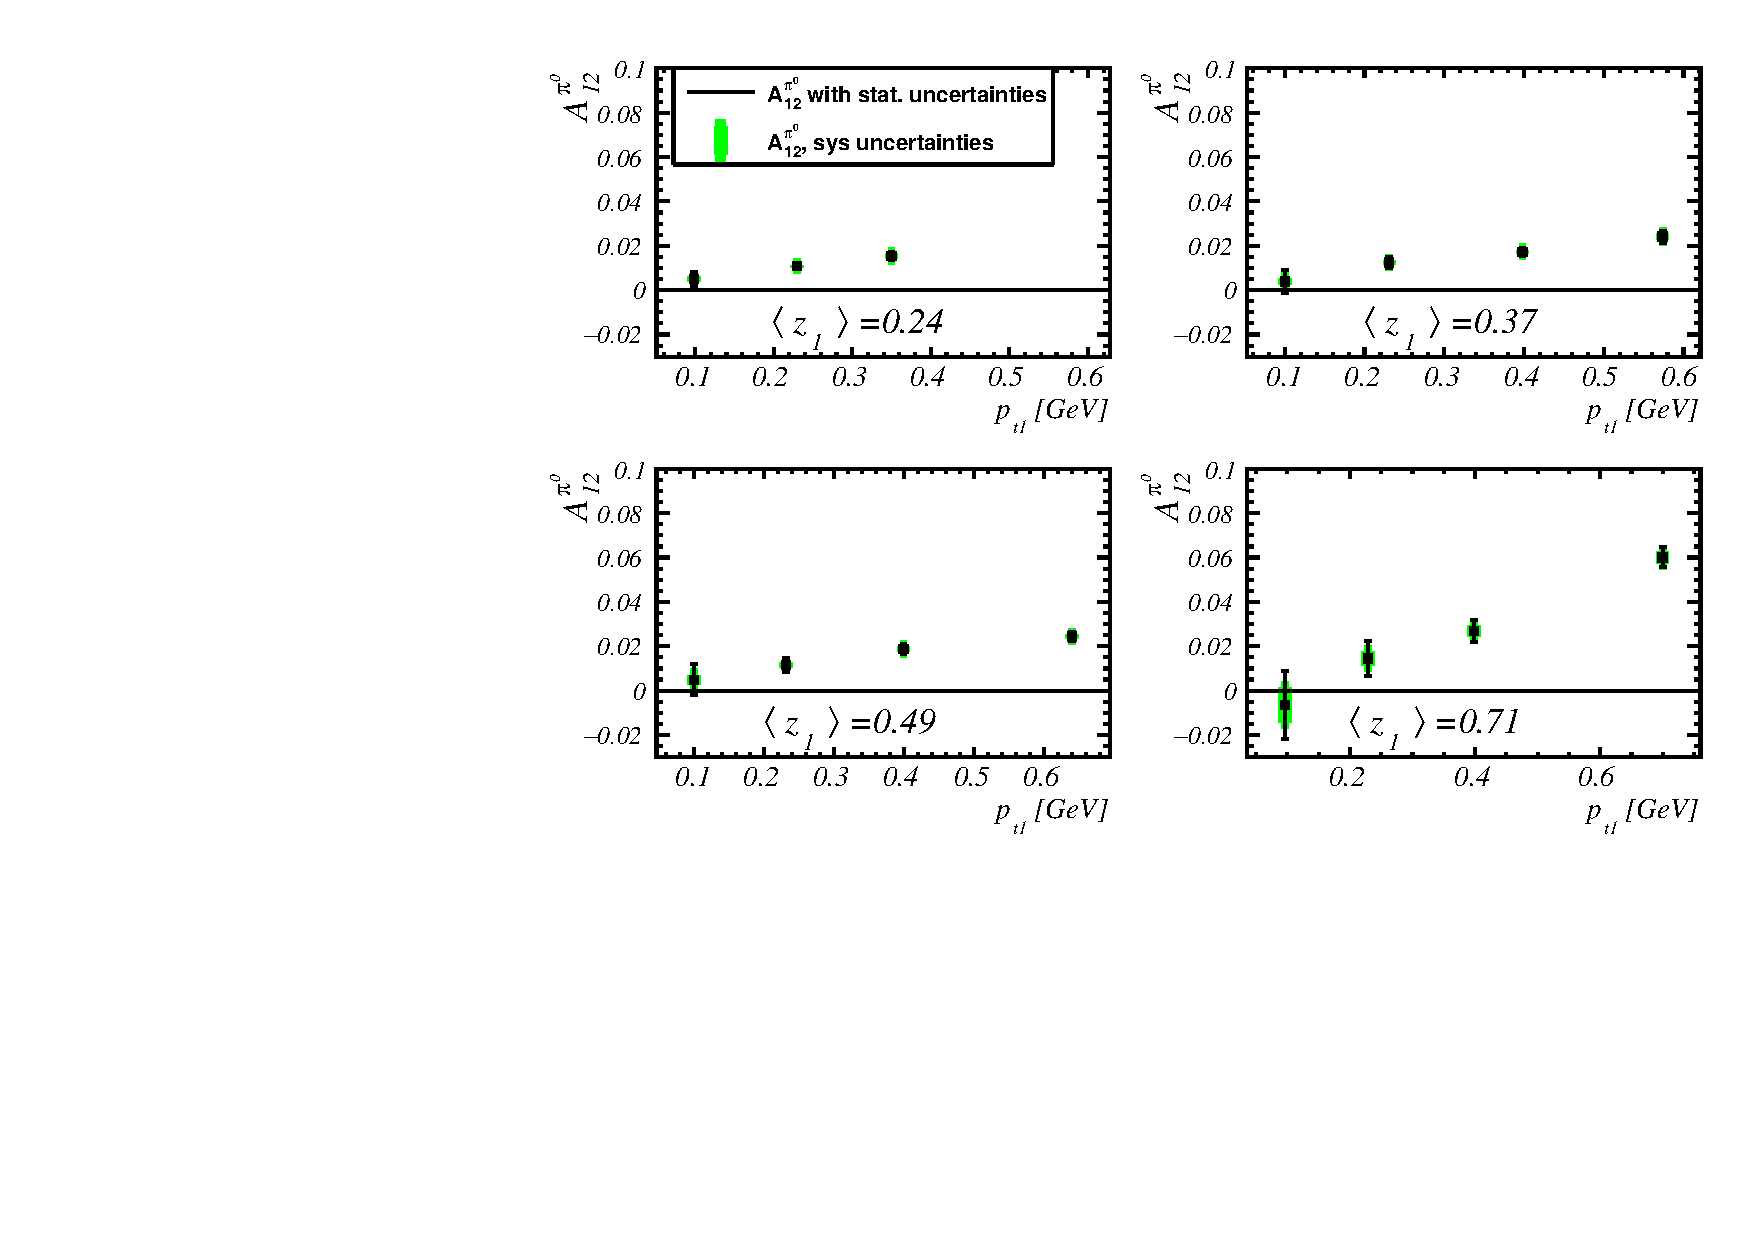
\includegraphics[width=0.95\textwidth]{figs_paper/pi0VsZPt.pdf}
\caption{Results for $A^{\pi^0}_{12}$ vs. $z_1,P_{t1}$. Significant asymmetries are observed, which rise with $z_1$ and $P_{t1}$.\label{fig:resPi0VsZPt}. See discussion in the text.}
\end{figure}

The results for the $\eta$ asymmetries have significantly larger uncertainties as the $\pi^0$ results. Figures~\ref{fig:resEtaZ1Z2} and~\ref{fig:resEtaZPt} show the results of $A^{\eta}_{12}$ versus $z_1,z_2$ and $z_1,P_{t1}$, respectively. The asymmetries are consistent with the $A^{\pi^0}_{12}$ results. This is shown explicitly in Fig.~\ref{fig:resEtaPi0ZPt} for the $z_1,P_{t1}$ binning.
\begin{figure}
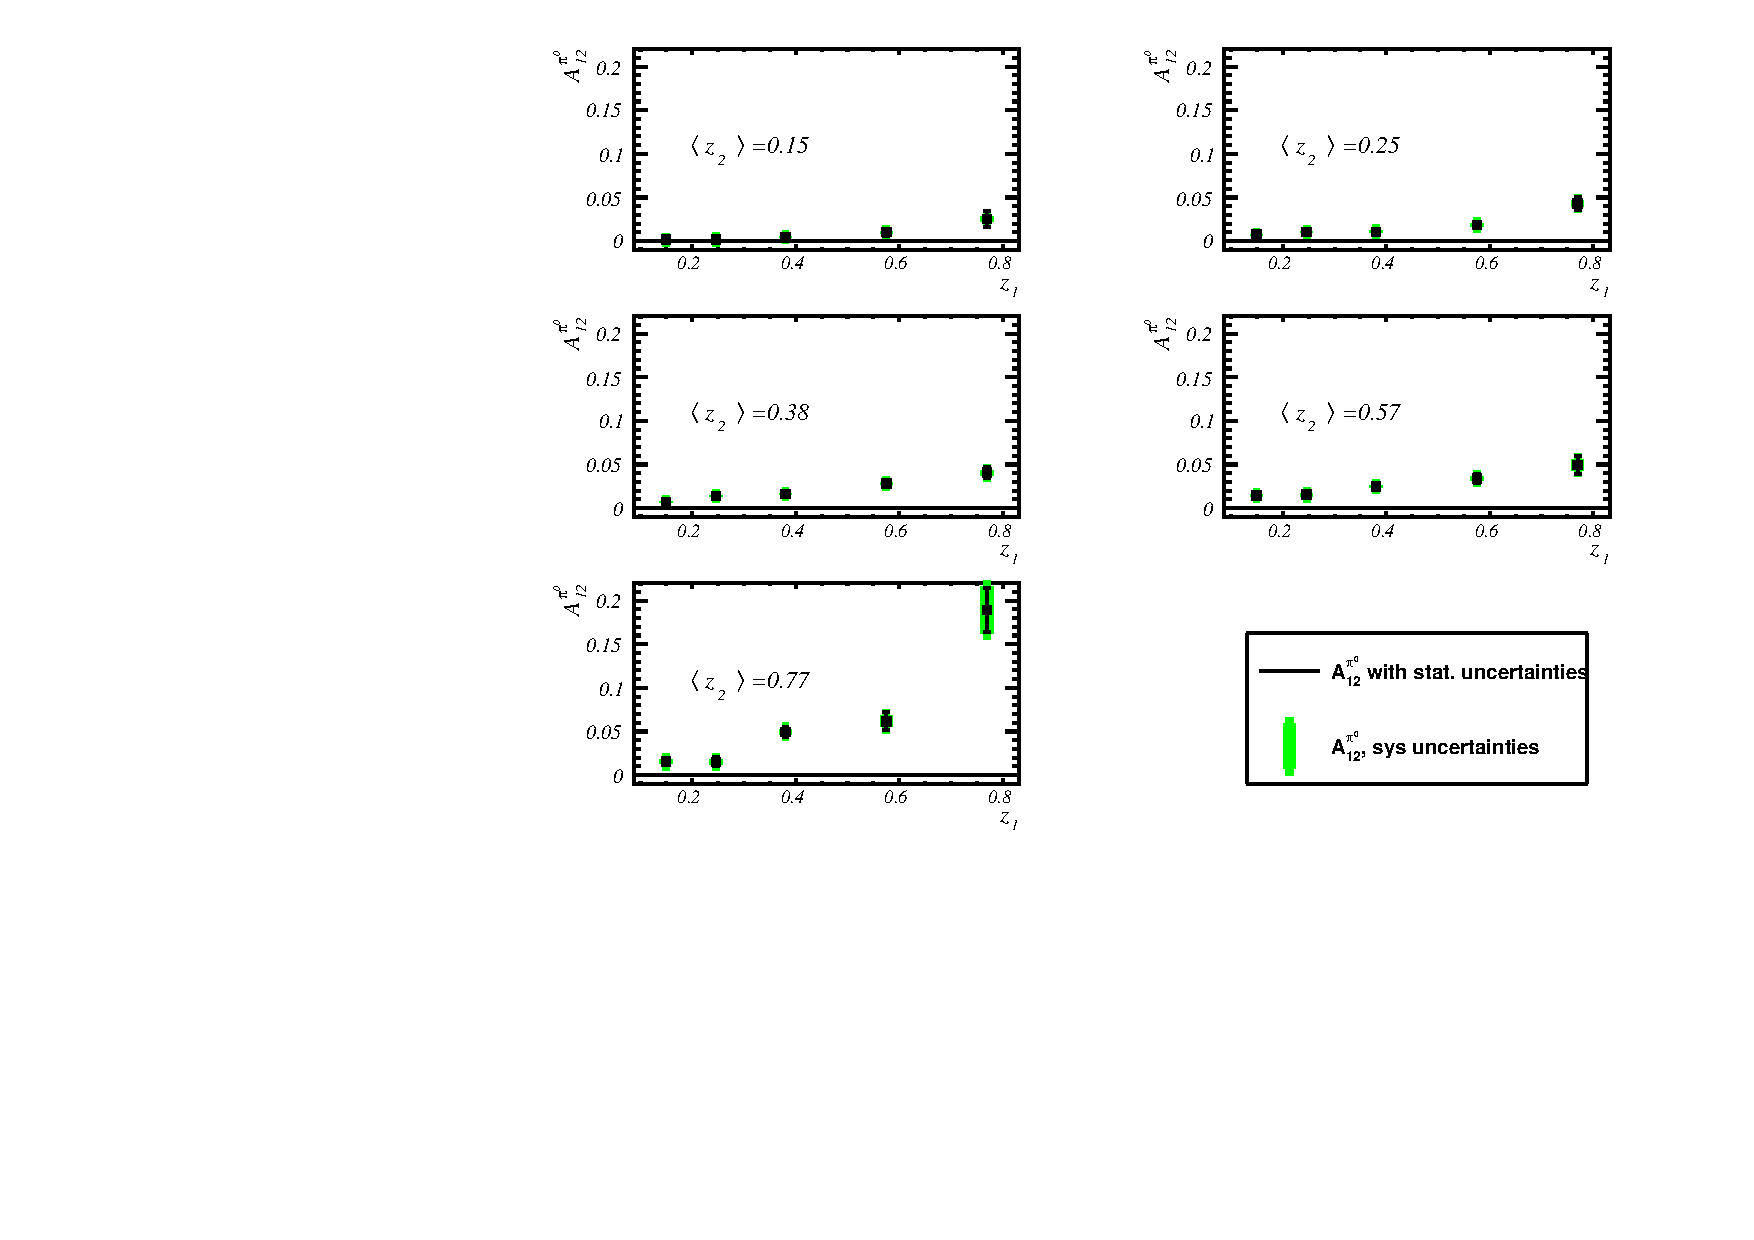
\includegraphics[width=0.95\textwidth]{figs_paper/pi0VsZ1Z2.pdf}
\caption{Results for $A^{\eta}_{12}$ vs $z_1, z_2$.\label{fig:resEtaZ1Z2}}
\end{figure}

\begin{figure}
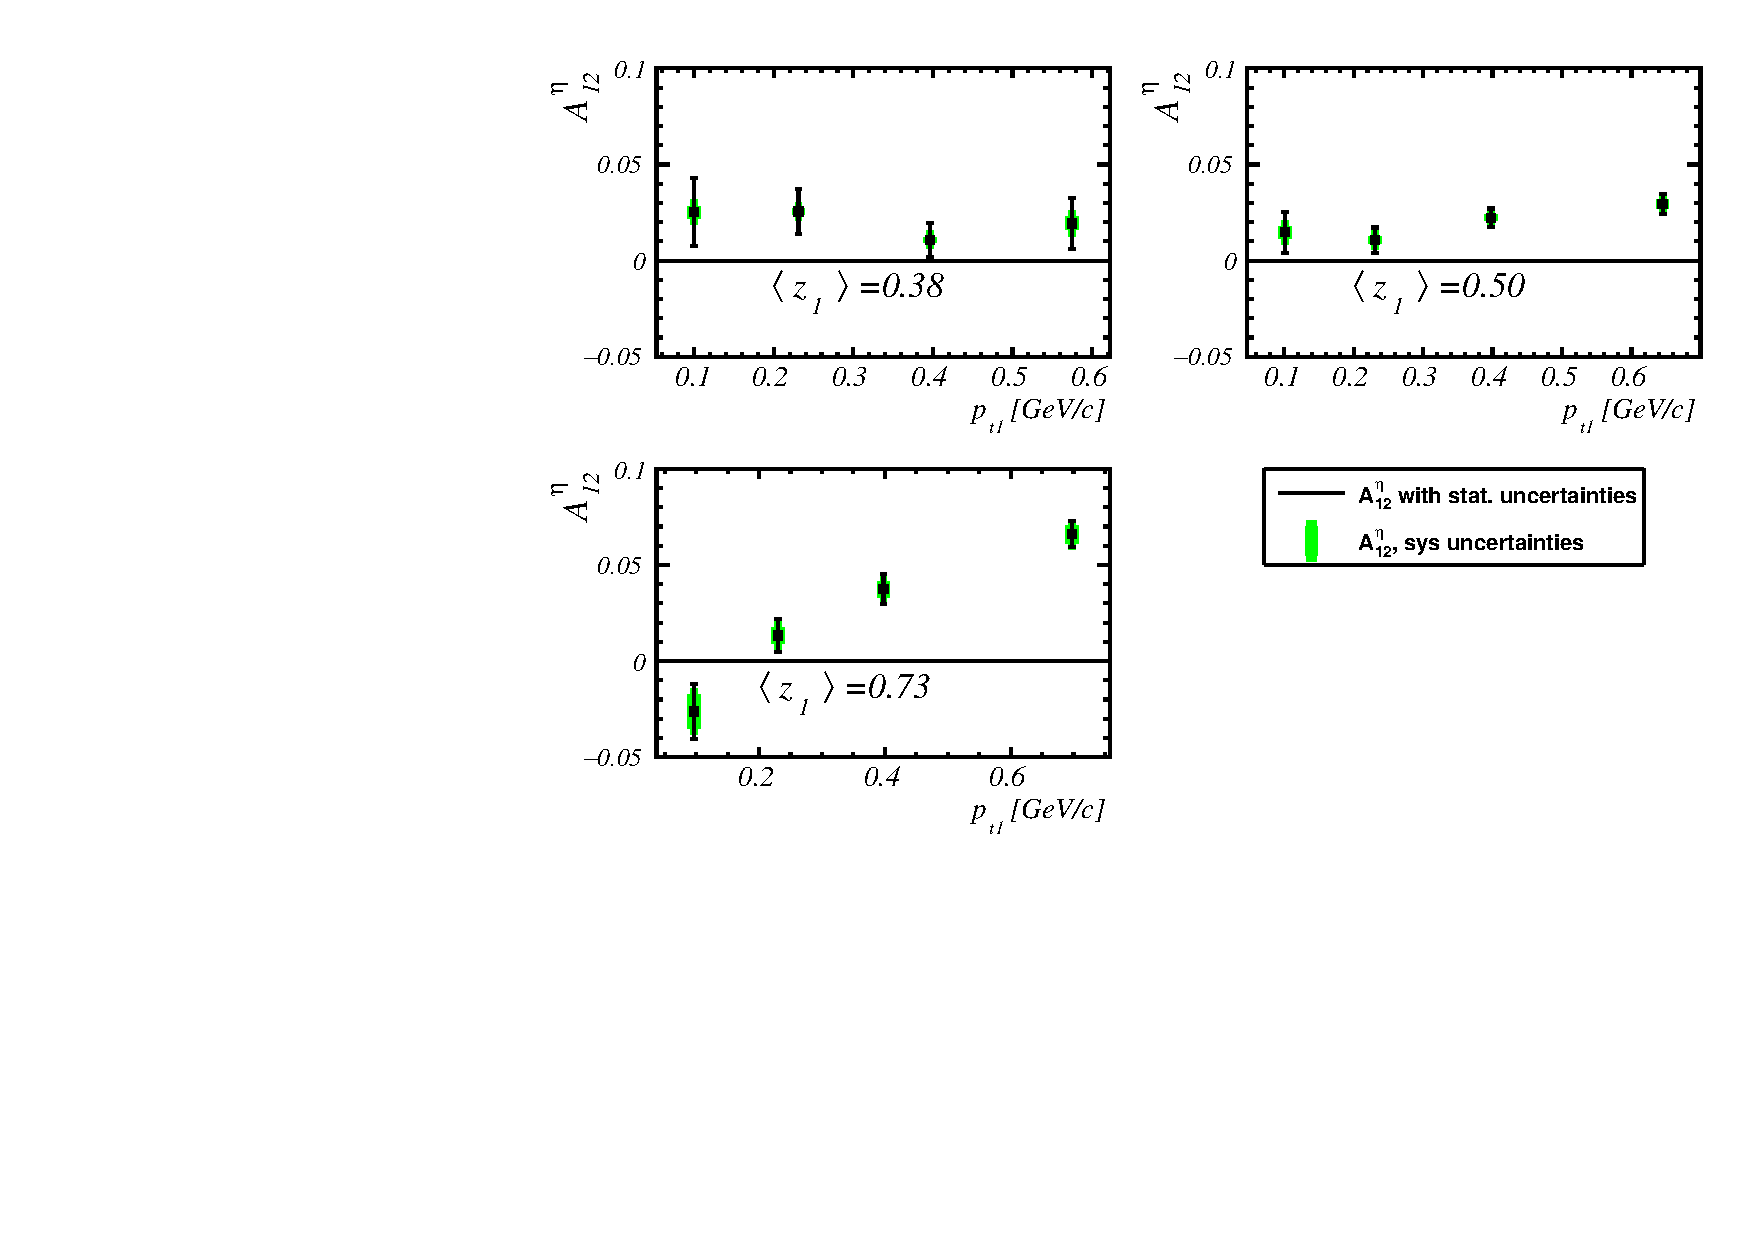
\includegraphics[width=0.95\textwidth]{figs_paper/etaVsZPt.pdf}
\caption{Results for $A^{\eta}_{12}$ vs $z_1, P_{t1}$.\label{fig:resEtaZPt}}
\end{figure}

\begin{figure}
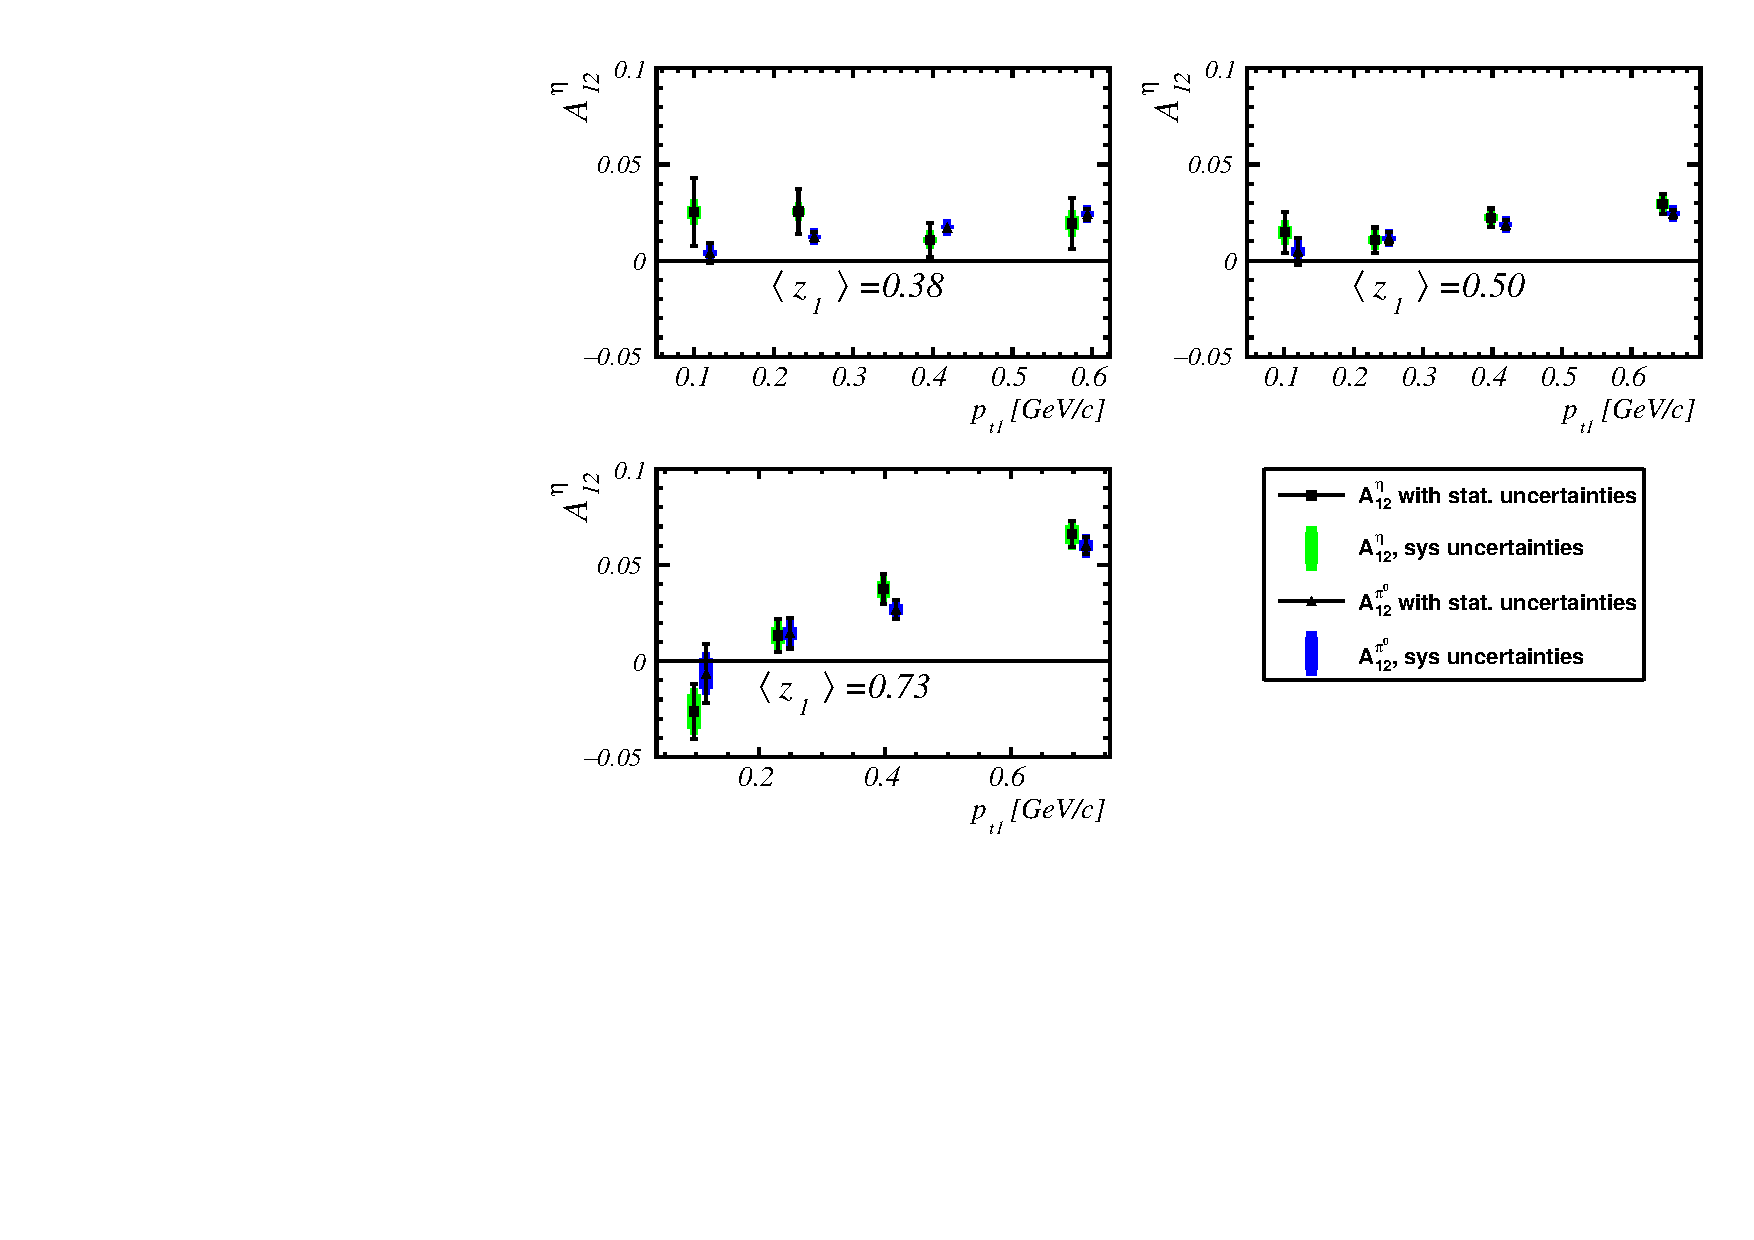
\includegraphics[width=0.95\textwidth]{figs_paper/etaPi0VsZPt.pdf}
\caption{Comparison of $A^{\pi^0}_{12}$ and $A^{\eta}_{12}$. Within the uncertainties, the two asymmetries are consistent. To make the comparison, a cut of $z_1>0.3$ is used for $A^{\pi^0}_{12}$ as well.\label{fig:resEtaPi0ZPt}}
\end{figure}

For charged pion pairs, Fig.~\ref{fig:resUlUcPt1Pt2} shows the results for $A^{UL}_{12}$ and $A^{UC}_{12}$ versus $P_{t1},P_{t2}$. Consistent with the previous measurement at BaBar~\cite{BabarCharged}, we observe significant asymmetries, which rise with $P_{t1}$ and $P_{t2}$. A direct quantitative comparison with the BaBar results is not attempted here, due to the different fiducial cuts used which result in sufficiently different kinematics covered in $z_1,z_2,P_{t1},P_{t2}$ space.
The magnitude of $A^{UL}_{12}$ is about twice as large as that of $A^{UC}_{12}$, consistent with previous measurements.

\begin{figure}
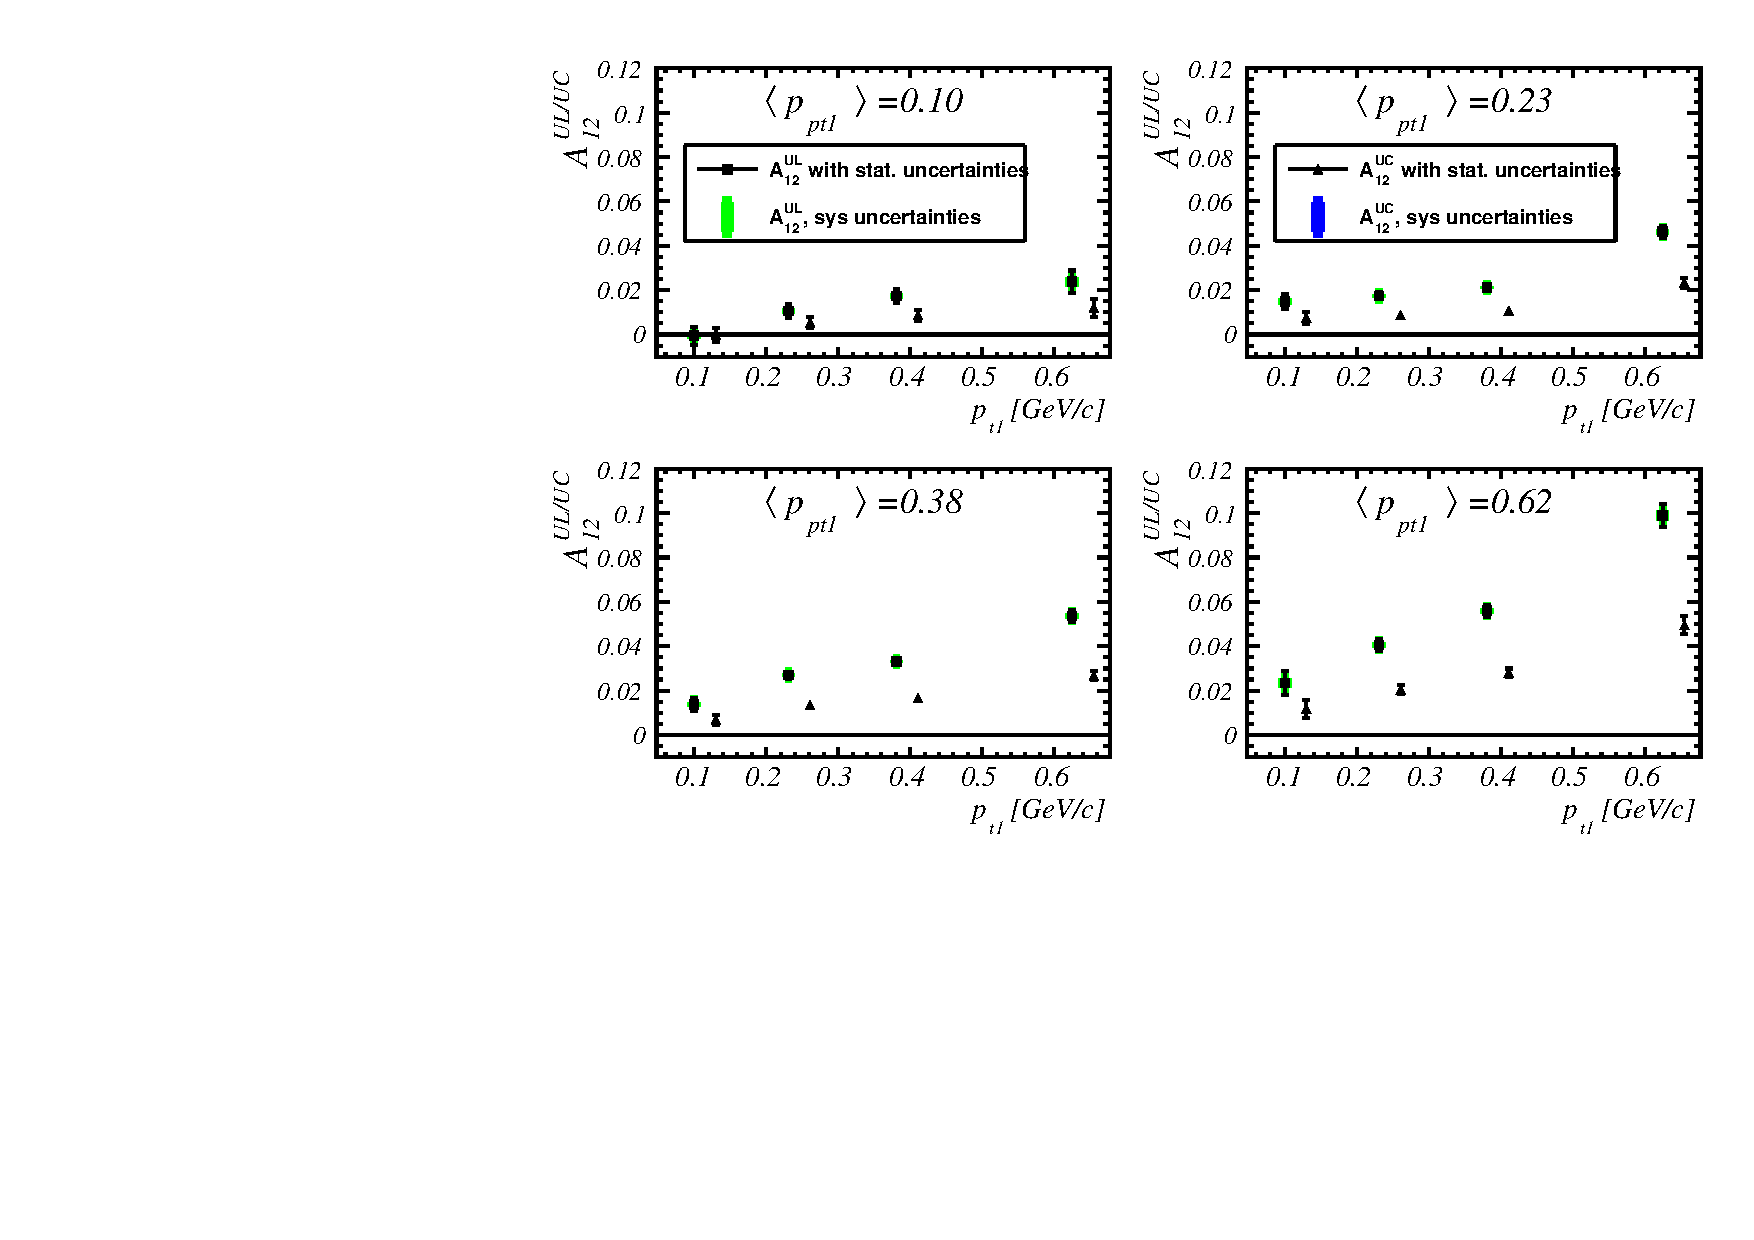
\includegraphics[width=0.95\textwidth]{figs_paper/ulUcPt1Pt2.pdf}
\caption{$A^{UL}_{12}$ and $A^{UC}_{12}$ for charged pion pairs vs $P_{t1}$ and $P_{t2}$. We observe significant asymmetries, which rise with $P_{t1}$ and $P_{t2}$. The magnitude of $A^{UL}_{12}$ is about twice as large as that of $A^{UC}_{12}$.\label{fig:resUlUcPt1Pt2}}	
\end{figure}

Since there are already published results from Belle for charged pion pairs in $z_1,z_2$ binning which covers roughly the same kinematic region, a comparison is made between the results presented in this report and the previous results. This comparison is shown in Fig.~\ref{fig:belleComp}. There are a number of noteworthy differences between the two analysis; The previous analysis does not apply opening angle cuts. Since this mainly impacts the $z$ distributions, a binning in both, $z_1$ and $z_2$ should mitigate the effect of this difference. The previous analysis uses a smearing correction to correct back to the $q\bar{q}$ axis extracted from simulation. Since this is not an observable and can only cleanly be defined at leading order, this correction is replaced with a correction back to the thrust axis in the present analysis. 
Finally, the previous Belle analysis corrects for the charm contribution using a $D^*$ sample. In this analysis, the charm contribution was not corrected for, since using the $D^*$ sample can introduce a bias in phase space and introduce larger uncertainties. Instead the charm contribution for each bin is given in the appendix, so it can be used for a global extraction. For this comparison, it is assumed that the signal coming from charm fragmentation vanishes. 
With the exception of one point in the third $z_1$ and $z_2$ bin, which seems to be an outlier, the agreement is good. However, a quantification of the agreement is difficult, since the uncertainties of the measurements are correlated. Disregarding this correlation and excluding the outlier, one arrives at a $\chi^2/N$ of $1.4$.
%Excluding the outlier and under the assumption that the $\chi^2/N$ is $1.4$.  
This seems to indicate that the assumption of a vanishing asymmetry for charm quarks is justified and that the difference between using the thrust axis and the so-called true $q\bar{q}$ axis is small.

\begin{figure}
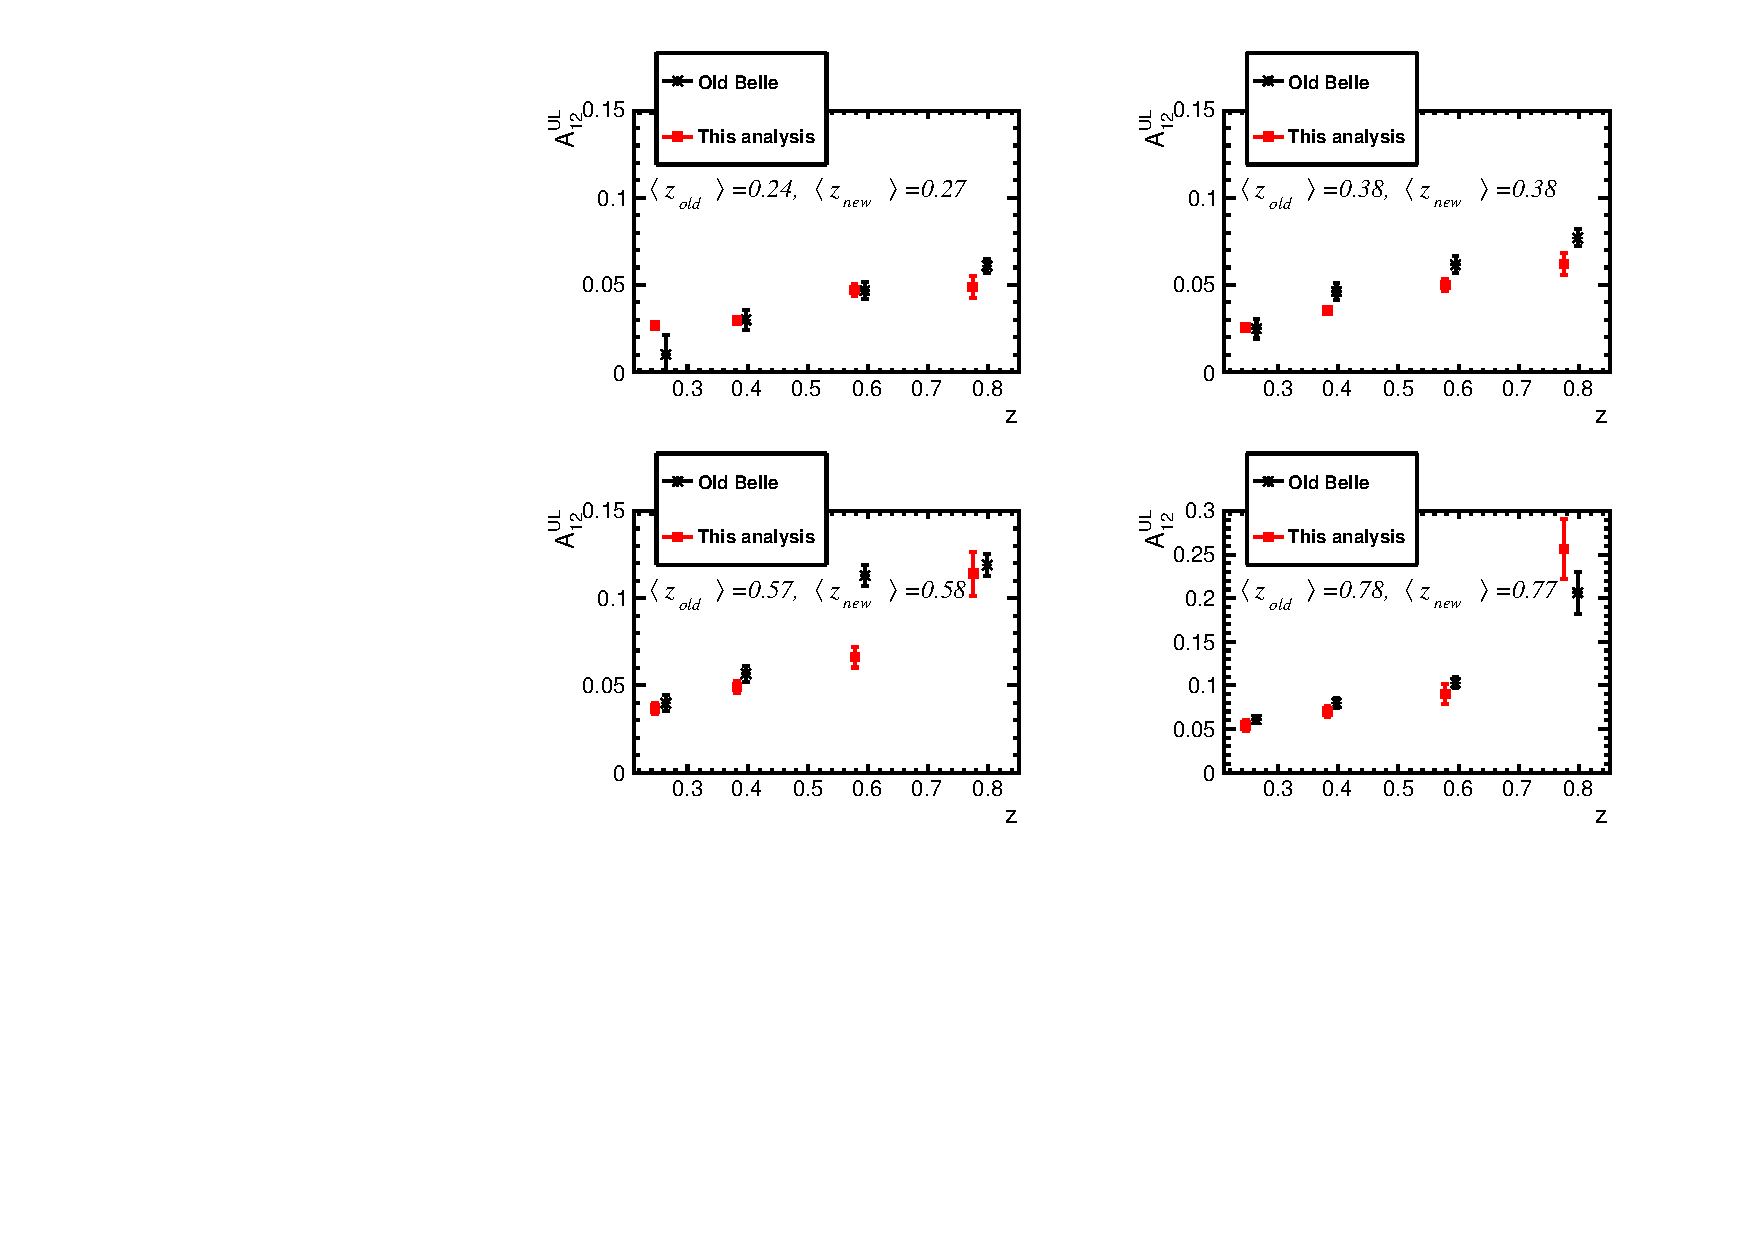
\includegraphics[width=0.95\textwidth]{figs_paper/BelleCompZ25.pdf}
\caption{\label{fig:belleComp} Comparison between the values for $A^{UL}_{12}$ extracted in this analysis and the previous Belle analysis in the $z_1$,$z_2$. To make the comparison, the  contribution of charm quarks was corrected for by assuming a vanishing asymmetry. The lowest $z$ bin was omitted, since the previous analysis used a cut of $z>0.2$. $z$ values are offset by 0.02 for better visibility.\label{fig:resOldBelleComp}}
\end{figure}

%on second thought, this might not make sense, since there is no reason to compare these. Maybe just the old Belle results?
%should be fine to include the eta here if the binning is z1, z2 differential. Otherwise the z>0.3 cut in the eta will distort the results
%\begin{figure}

%\caption{pi0, eta, uc, ul and old belle results on same panel}
%\end{figure}

\section{Summary and Conclusion}
\label{sec:summary}
Summarizing, an analysis of azimuthal asymmetries related to the Collins mechanism has been presented for pairs of back-to-back neutral and charged pions as well as $\eta$ mesons and charged pions. The analysis substantially differs from previous Belle analyses in that results are only presented in the thrust-axis frame without correcting to the q-qbar axis, the opening angle of the hadrons to the thrust axis was limited to 0.3 rad, which effectively corresponds to a z-dependent upper limit on $P_t$, and asymmetries were not corrected for charm contributions. Instead , the charm fraction is included and can be used in future analyses when relevant results on charm azimuthal asymmetries become available, e.g., from Belle II. More importantly, this measurement significantly expands the scope of previous Belle measurements by a) including neutral pions and eta mesons; and b) exploring the transverse-momentum dependence of the azimuthal asymmetries.
 Significant asymmetries for all channels are observed. Asymmetries rise, within the given kinematic coverage, with $z$ and $P_t$. The signal for $\eta$ and $\pi^0$ mesons agrees within uncertainties. It was also shown that the results for charged pion pairs agree well with previous measurements.

\clearpage
\bibliography{Citations}
\clearpage


\appendix
\section{Supplemental Tables}



 \begin{table}[h]
\centering
\begin{tabular}{|c||c|c|c|c|c|c|}
\hline
$z_1$ & $\pi^{\pm}\pi^{\pm}$ & $\pi^{\pm}\pi^0$ & $\eta\pi^{\pm}$ & $\pi^0\pi^{\pm}$ $(z>0.3)$ & $\pi^{\pm}\pi^{\pm}$ $(z>0.3)$ \\ \hline\hline
%[0.1,0.2]       &	30.59	&	39.08	&		&		&			\\ \hline
[0.2,0.3]	&	22.24	&	23.90	&		&		&		\\ \hline
[0.3,0.4]	&	18.34	&	18.64	&	19.71	&	15.98	&	15.74	\\ \hline
[0.4,0.5]	&	16.48	&	16.17	&	16.85	&	13.73	&	13.72	\\ \hline
[0.5,0.6]	&	14.50	&	13.53	&	15.63	&	11.33	&	11.86	\\ \hline
[0.6,0.7]	&	10.12	&	8.85	&	13.04	&	7.20	&	8.30	\\ \hline
[0.7,1.0]	&	4.66	&	3.63	&	7.18	&	2.90	&	4.08	\\ \hline\end{tabular}
\caption[Charm ratio in $z_1$ bins]{Charm ratio in $z_1$ bins. All numbers are in percent.}
\label{tab:sinzcharmratio}
\end{table}


\begin{table}[h]
\centering
\begin{tabular}{|c|c||c|c|c|c|c|c|}
\hline
 $z_1$& $z_2$ & $\pi^{\pm}\pi^{\pm}$ & $\pi^{\pm}\pi^0$ & $\eta\pi^{\pm}$ & $\pi^0\pi^{\pm}$ $(z>0.3)$ & $\pi^{\pm}\pi^{\pm}$ $(z>0.3)$ \\ \hline\hline
[0.1,0.2]	&	[0.1,0.2]	&	36.75	&	41.87	&		&		&		\\ \hline
[0.1,0.2]	&	[0.2,0.3]	&	30.63	&	35.32	&		&		&		\\ \hline
[0.1,0.2]	&	[0.3,0.5]	&	24.97	&	28.98	&		&		&		\\ \hline
[0.1,0.2]	&	[0.5,0.7]	&	18.98	&	22.47	&		&		&		\\ \hline
[0.1,0.2]	&	[0.7,1.0]	&	6.45	&	7.80	&		&		&		\\ \hline \hline
[0.2,0.3]	&	[0.1,0.2]	&	30.65	&	32.92	&		&		&		\\ \hline
[0.2,0.3]	&	[0.2,0.3]	&	25.52	&	27.40	&		&		&		\\ \hline
[0.2,0.3]	&	[0.3,0.5]	&	20.55	&	22.11	&		&		&		\\ \hline
[0.2,0.3]	&	[0.5,0.7]	&	15.75	&	16.82	&		&		&		\\ \hline
[0.2,0.3]	&	[0.7,1.0]	&	5.44	&	5.76	&		&		&		\\ \hline\hline
[0.3,0.5]	&	[0.1,0.2]	&	25.13	&	25.47	&		&		&		\\ \hline
[0.3,0.5]	&	[0.2,0.3]	&	20.71	&	20.85	&		&		&		\\ \hline
[0.3,0.5]	&	[0.3,0.5]	&	15.96	&	16.28	&	19.85	&	16.28	&	16.05	\\ \hline
[0.3,0.5]	&	[0.5,0.7]	&	11.70	&	12.01	&	14.66	&	12.01	&	11.69	\\ \hline
[0.3,0.5]	&	[0.7,1.0]	&	4.10	&	3.95	&	4.66	&	3.95	&	4.43	\\ \hline\hline
[0.5,0.7]	&	[0.1,0.2]	&	19.22	&	18.12	&		&		&		\\ \hline
[0.5,0.7]	&	[0.2,0.3]	&	15.92	&	14.90	&		&		&		\\ \hline
[0.5,0.7]	&	[0.3,0.5]	&	11.75	&	11.13	&	16.13	&	11.13	&	11.74	\\ \hline
[0.5,0.7]	&	[0.5,0.7]	&	8.03	&	7.74	&	11.02	&	7.74	&	7.78	\\ \hline
[0.5,0.7]	&	[0.7,1.0]	&	2.74	&	2.65	&	3.22	&	2.65	&	2.89	\\ \hline\hline
[0.7,1.0]	&	[0.1,0.2]	&	6.88	&	5.47	&		&		&		\\ \hline
[0.7,1.0]	&	[0.2,0.3]	&	5.72	&	4.59	&		&		&		\\ \hline
[0.7,1.0]	&	[0.3,0.5]	&	4.10	&	3.20	&	7.82	&	3.20	&	4.44	\\ \hline
[0.7,1.0]	&	[0.5,0.7]	&	2.77	&	1.91	&	5.11	&	1.91	&	2.91	\\ \hline
[0.7,1.0]	&	[0.7,1.0]	&	1.11	&	0.90	&	2.40	&	0.90	&	1.28	\\ \hline
\end{tabular}
\caption[Charm ratio in combined $z_{1}$--$z_{2}$ bins]{Charm ratio in combined $z_{1}$--$z_{2}$ bins. All numbers are in percent.}
\label{tab:comzcharmratio}
\end{table}


\begin{table}[h]
\centering
\begin{tabular}{|c||c|c|c|c|c|c|}
\hline
$P_{t1}$ [GeV]  &$\pi^{\pm}\pi^{\pm}$ & $\pi^{\pm}\pi^0$ & $\eta\pi^{\pm}$ & $\pi^0\pi^{\pm}$ $(z>0.3)$ & $\pi^{\pm}\pi^{\pm}$ $(z>0.3)$ \\ \hline\hline
[0,0.15]	&	19.74	&	21.44	&	15.67	&	13.32	&	12.91	\\ \hline
[0.15,0.30]	&	19.60	&	21.08	&	16.16	&	13.57	&	13.20	\\ \hline
[0.30,0.50]	&	18.76	&	19.40	&	18.19	&	14.60	&	14.38	\\ \hline
[0.50,3.0]	&	18.75	&	18.19	&	21.10	&	15.45	&	15.54	\\ \hline
\end{tabular}
\caption[Charm ratio in $P_{t1}$ bins]{Charm ratio in $P_{t1}$ bins. All numbers are in percent.}
\label{tab:sinptcharmratio}
\end{table}

\begin{table}[H]
\centering
\begin{tabular}{|c|c||c|c|c|c|c|c|}
\hline
$P_{t1}$ [GeV] & $P_{t2}$ [GeV] &$\pi^{\pm}\pi^{\pm}$ & $\pi^{\pm}\pi^0$ & $\eta\pi^{\pm}$ & $\pi^0\pi^{\pm}$ $(z>0.3)$ & $\pi^{\pm}\pi^{\pm}$ $(z>0.3)$ \\ \hline\hline
[0,0.15]	&	[0,0.15]	&	20.15	&	21.93	&	13.80	&	11.75	&	11.81	\\ \hline
[0,0.15]	&	[0.15,0.30]	&	20.07	&	21.82	&	14.74	&	12.32	&	12.01	\\ \hline
[0,0.15]	&	[0.30,0.50]	&	19.28	&	20.87	&	15.86	&	13.54	&	13.15	\\ \hline
[0,0.15]	&	[0.50,3.0]	&	19.44	&	21.33	&	17.92	&	15.43	&	14.58	\\ \hline\hline
[0.15,0.30]	&	[0,0.15]	&	20.10	&	21.55	&	14.37	&	12.09	&	12.05	\\ \hline
[0.15,0.30]	&	[0.15,0.30]	&	19.92	&	21.42	&	14.71	&	12.43	&	12.29	\\ \hline
[0.15,0.30]	&	[0.30,0.50]	&	19.12	&	20.59	&	16.72	&	13.87	&	13.52	\\ \hline
[0.15,0.30]	&	[0.50,3.0]	&	19.22	&	20.79	&	18.32	&	15.65	&	14.69	\\ \hline\hline
[0.30,0.50]	&	[0,0.15]	&	19.36	&	19.91	&	16.41	&	13.10	&	13.31	\\ \hline
[0.30,0.50]	&	[0.15,0.30]	&	19.15	&	19.79	&	16.78	&	13.48	&	13.51	\\ \hline
[0.30,0.50]	&	[0.30,0.50]	&	18.24	&	18.87	&	18.60	&	14.88	&	14.67	\\ \hline
[0.30,0.50]	&	[0.50,3.0]	&	18.09	&	18.97	&	20.64	&	16.70	&	15.84	\\ \hline\hline
[0.50,3.0]	&	[0,0.15]	&	19.55	&	18.84	&	18.79	&	14.10	&	14.69	\\ \hline
[0.50,3.0]	&	[0.15,0.30]	&	19.38	&	18.66	&	19.86	&	14.38	&	14.98	\\ \hline
[0.50,3.0]	&	[0.30,0.50]	&	18.14	&	17.63	&	21.46	&	15.74	&	15.89	\\ \hline
[0.50,3.0]	&	[0.50,3.0]	&	16.98	&	17.37	&	23.69	&	17.37	&	16.23	\\ \hline
\end{tabular}
\caption[Charm ratio in combined $(P_{t1},P_{t2})$ bins]{Charm ratio in $(P_{t1},P_{t2})$ bins. All numbers are in percent.}
\label{tab:comptcharmratio}
\end{table}

\begin{table}[h]
\centering
\begin{tabular}{|c|c|c|c|}
\hline
$z_1$ & $P_{t1}$ [GeV] &$\pi^{\pm}\pi^{\pm}$ & $\pi^{\pm}\pi^0$ \\ \hline\hline
[0.2,0.3]	&	[0,0.15]	&	22.85	&	24.63	\\ \hline
[0.2,0.3]	&	[0.15,0.30]	&	22.40	&	24.08	\\ \hline
[0.2,0.3]	&	[0.30,0.50]	&	21.88	&	22.98	\\ \hline
[0.2,0.3]	&	[0.50,3.0]	&		&		\\ \hline\hline
[0.3,0.5]	&	[0,0.15]	&	16.13	&	16.55	\\ \hline
[0.3,0.5]	&	[0.15,0.30]	&	16.46	&	16.85	\\ \hline
[0.3,0.5]	&	[0.30,0.50]	&	17.94	&	18.07	\\ \hline
[0.3,0.5]	&	[0.50,3.0]	&	20.79	&	20.38	\\ \hline\hline
[0.5,0.7]	&	[0,0.15]	&	10.54	&	15.78	\\ \hline
[0.5,0.7]	&	[0.15,0.30]	&	10.97	&	16.05	\\ \hline
[0.5,0.7]	&	[0.30,0.50]	&	12.53	&	17.27	\\ \hline
[0.5,0.7]	&	[0.50,3.0]	&	15.78	&	18.54	\\ \hline\hline
[0.7,1.0]	&	[0,0.15]	&	3.37	&	9.53	\\ \hline
[0.7,1.0]	&	[0.15,0.30]	&	3.96	&	10.01	\\ \hline
[0.7,1.0]	&	[0.30,0.50]	&	4.68	&	11.34	\\ \hline
[0.7,1.0]	&	[0.50,3.0]	&	6.42	&	13.75	\\ \hline
\end{tabular}
\caption[Charm ratio in $(z_{1},P_{t1})$ bins]{Charm ratio in $(z_{1},P_{t1})$ bins. All numbers are in percent.}
\label{tab:zptcharmratio}
\end{table}




\begin{table}[H]\tiny
\centering
\renewcommand{\arraystretch}{1.5}
\begin{tabular}{|c| c| c| c| c| c| c| c| c| c| c| c| c| c| c|}
\hline
$z_1$ & $\langle  z_1\rangle$ & $\langle  P_{t1}\rangle$  [GeV] & $z_2$ & $\langle  z_2 \rangle$ & $\langle  P_{t2}\rangle$ [GeV]  & $\langle\frac{\sin^2(\theta)}{1+\cos^2(\theta)}\rangle$& $A_{12}^{\pi^0}$ [\%]  \\ \hline
[0.2,0.3]	&	0.246	&	0.238	&	[0.2,1.0]	&	0.355	&	0.317	&	0.905	&	1.25  $\pm$ 0.12  $\pm$ 0.06    \\ \hline
[0.3,0.4]	&	0.345	&	0.321	&	[0.2,1.0]	&	0.356	&	0.317	&	0.906	&	1.72  $\pm$ 0.13  $\pm$ 0.04    \\ \hline
[0.4,0.5]	&	0.445	&	0.392	&	[0.2,1.0]	&	0.357	&	0.318	&	0.907	&	1.72  $\pm$ 0.16  $\pm$ 0.06    \\ \hline
[0.5,0.6]	&	0.544	&	0.449	&	[0.2,1.0]	&	0.358	&	0.318	&	0.905	&	2.08  $\pm$ 0.22  $\pm$ 0.11    \\ \hline
[0.6,0.7]	&	0.643	&	0.485	&	[0.2,1.0]	&	0.359	&	0.32	&	0.904	&	2.51  $\pm$ 0.28  $\pm$ 0.13    \\ \hline
[0.7,1.0]	&	0.77	&	0.442	&	[0.2,1.0]	&	0.359	&	0.321	&	0.902	&	3.86  $\pm$ 0.36  $\pm$ 0.2  	\\ \hline
\hline
[0.1,0.2]	&	0.149	&	0.146	&	[0.1,0.2]	&	0.148	&	0.15	&	0.906	&0.16  $\pm$ 0.19  $\pm$ 0.04 	\\ \hline
[0.1,0.2]	&	0.149	&	0.147	&	[0.2,0.3]	&	0.246	&	0.241	&	0.905	&0.18  $\pm$ 0.22  $\pm$ 0.06 	\\ \hline
[0.1,0.2]	&	0.149	&	0.147	&	[0.3,0.5]	&	0.381	&	0.348	&	0.905	&0.47  $\pm$ 0.22  $\pm$ 0.07 	\\ \hline
[0.1,0.2]	&	0.149	&	0.147	&	[0.5,0.7]	&	0.577	&	0.458	&	0.905	&1.02  $\pm$ 0.41  $\pm$ 0.11 	\\ \hline
[0.1,0.2]	&	0.149	&	0.148	&	[0.7,1.0]	&	0.776	&	0.425	&	0.903	&2.52  $\pm$ 0.92  $\pm$ 0.25 	\\ \hline
\hline
[0.2,0.3]	&	0.246	&	0.238	&	[0.1,0.2]	&	0.148	&	0.15	&	0.906	&0.74  $\pm$ 0.15  $\pm$ 0.04 	\\ \hline
[0.2,0.3]	&	0.246	&	0.238	&	[0.2,0.3]	&	0.246	&	0.242	&	0.906	&1.07  $\pm$ 0.19  $\pm$ 0.05 	\\ \hline
[0.2,0.3]	&	0.246	&	0.238	&	[0.3,0.5]	&	0.381	&	0.348	&	0.905	&1.07  $\pm$ 0.19  $\pm$ 0.11 	\\ \hline
[0.2,0.3]	&	0.246	&	0.238	&	[0.5,0.7]	&	0.578	&	0.46	&	0.905	&1.85  $\pm$ 0.37  $\pm$ 0.12 	\\ \hline
[0.2,0.3]	&	0.246	&	0.24	&	[0.7,1.0]	&	0.777	&	0.434	&	0.903	&4.33  $\pm$ 0.77  $\pm$ 0.32 	\\ \hline
\hline
[0.3,0.5]	&	0.38	&	0.345	&	[0.1,0.2]	&	0.148	&	0.15	&	0.908	&0.71  $\pm$ 0.13  $\pm$ 0.04 	\\ \hline
[0.3,0.5]	&	0.38	&	0.345	&	[0.2,0.3]	&	0.246	&	0.242	&	0.907	&1.4  $\pm$ 0.15  $\pm$ 0.05  	\\ \hline
[0.3,0.5]	&	0.38	&	0.346	&	[0.3,0.5]	&	0.381	&	0.348	&	0.906	&1.63  $\pm$ 0.16  $\pm$ 0.06 	\\ \hline
[0.3,0.5]	&	0.381	&	0.346	&	[0.5,0.7]	&	0.578	&	0.462	&	0.906	&2.83  $\pm$ 0.3  $\pm$ 0.1   	\\ \hline
[0.3,0.5]	&	0.38	&	0.347	&	[0.7,1.0]	&	0.777	&	0.438	&	0.905	&4.07  $\pm$ 0.65  $\pm$ 0.28 	\\ \hline
\hline
[0.5,0.7]	&	0.575	&	0.457	&	[0.1,0.2]	&	0.149	&	0.151	&	0.906	&1.46  $\pm$ 0.22  $\pm$ 0.09 	\\ \hline
[0.5,0.7]	&	0.575	&	0.459	&	[0.2,0.3]	&	0.246	&	0.242	&	0.905	&1.54  $\pm$ 0.26  $\pm$ 0.16 	\\ \hline
[0.5,0.7]	&	0.576	&	0.461	&	[0.3,0.5]	&	0.382	&	0.348	&	0.905	&2.49  $\pm$ 0.26  $\pm$ 0.1  	\\ \hline
[0.5,0.7]	&	0.576	&	0.464	&	[0.5,0.7]	&	0.579	&	0.464	&	0.905	&3.39  $\pm$ 0.49  $\pm$ 0.24 	\\ \hline
[0.5,0.7]	&	0.576	&	0.466	&	[0.7,1.0]	&	0.777	&	0.442	&	0.904	&4.94  $\pm$ 1.06  $\pm$ 0.6  	\\ \hline
\hline
[0.7,1.0]	&	0.769	&	0.425	&	[0.1,0.2]	&	0.149	&	0.151	&	0.902	&1.56  $\pm$ 0.45  $\pm$ 0.26 	\\ \hline
[0.7,1.0]	&	0.77	&	0.438	&	[0.2,0.3]	&	0.246	&	0.242	&	0.902	&1.53  $\pm$ 0.53  $\pm$ 0.28 	\\ \hline
[0.7,1.0]	&	0.77	&	0.443	&	[0.3,0.5]	&	0.382	&	0.349	&	0.901	&4.95  $\pm$ 0.57  $\pm$ 0.31 	\\ \hline
[0.7,1.0]	&	0.77	&	0.45	&	[0.5,0.7]	&	0.578	&	0.466	&	0.903	&6.17  $\pm$ 1.04  $\pm$ 0.64 	\\ \hline
[0.7,1.0]	&	0.766	&	0.465	&	[0.7,1.0]	&	0.771	&	0.461	&	0.903	&18.92 $\pm$ 2.49  $\pm$ 2.64	\\ \hline
\end{tabular}
\caption[Collins asymmetries $A_{12}^{\eta}$ binned in $z$]{Collins asymmetries  $A_{12}^{\eta}$ binned in $z$. Uncertainties are, first, statistical and, second, systematic.}
\label{tab:finalpi0zbin}
\end{table}

\begin{table}[H]\tiny
\centering
\renewcommand{\arraystretch}{1.5}
\begin{tabular}{|c| c| c| c| c| c| c| c| c| c|c| c| c| c| c|}
\hline
$z_1$ & $\langle  z_1\rangle$ & $\langle  P_{t1} \rangle$  [GeV] & $z_2$ & $\langle  z_2 \rangle$ & $\langle  P_{t2}  \rangle$ [GeV] & $\langle\frac{\sin^2(\theta)}{1+\cos^2(\theta)}\rangle$ & $A_{12}^{\eta}$ [\%]  \\ \hline
[0.2,0.3]	&		&		&	[0.2,1.0]	&		&		&		&		$\pm$			/+		\\ \hline
[0.3,0.4]	&	0.348	&	0.303	&	[0.2,1.0]	&	0.441	&	0.375	&	0.906	&2.52  $\pm$ 0.89  $\pm$ 0.11   \\ \hline
[0.4,0.5]	&	0.446	&	0.375	&	[0.2,1.0]	&	0.442	&	0.376	&	0.907	&2.61  $\pm$ 0.65  $\pm$ 0.14   \\ \hline
[0.5,0.6]	&	0.545	&	0.433	&	[0.2,1.0]	&	0.443	&	0.376	&	0.907	&2.82  $\pm$ 0.6  $\pm$ 0.2     \\ \hline
[0.6,0.7]	&	0.644	&	0.469	&	[0.2,1.0]	&	0.442	&	0.378	&	0.908	&2.63  $\pm$ 0.65  $\pm$ 0.31   \\ \hline
[0.7,1.0]	&	0.774	&	0.43	&	[0.2,1.0]	&	0.441	&	0.379	&	0.906	&2.8  $\pm$ 0.64  $\pm$ 0.42    \\ \hline
\hline
[0.1,0.2]	&		&		&	[0.1,0.2]	&		&		&		&							\\ \hline
[0.1,0.2]	&		&		&	[0.2,0.3]	&		&		&		&							\\ \hline
[0.1,0.2]	&		&		&	[0.3,0.5]	&		&		&		&							\\ \hline
[0.1,0.2]	&		&		&	[0.5,0.7]	&		&		&		&							\\ \hline
[0.1,0.2]	&		&		&	[0.7,1.0]	&		&		&		&							\\ \hline
\hline
[0.2,0.3]	&		&		&	[0.1,0.2]	&		&		&		&							\\ \hline
[0.2,0.3]	&		&		&	[0.2,0.3]	&		&		&		&							\\ \hline
[0.2,0.3]	&		&		&	[0.3,0.5]	&		&		&		&							\\ \hline
[0.2,0.3]	&		&		&	[0.5,0.7]	&		&		&		&							\\ \hline
[0.2,0.3]	&		&		&	[0.7,1.0]	&		&		&		&							\\ \hline
\hline
[0.3,0.5]	&		&		&	[0.1,0.2]	&		&		&		&							\\ \hline
[0.3,0.5]	&		&		&	[0.2,0.3]	&		&		&		&							\\ \hline
[0.3,0.5]	&	0.386	&	0.331	&	[0.3,0.5]	&	0.381	&	0.347	&	0.906	&	2.15  $\pm$ 0.63  $\pm$ 0.1     \\ \hline
[0.3,0.5]	&	0.387	&	0.331	&	[0.5,0.7]	&	0.578	&	0.461	&	0.907	&	3.59  $\pm$ 1.13  $\pm$ 0.19    \\ \hline
[0.3,0.5]	&	0.387	&	0.332	&	[0.7,1.0]	&	0.777	&	0.434	&	0.905	&	3.25  $\pm$ 2.38  $\pm$ 0.5  	\\ \hline
\hline
[0.5,0.7]	&		&		&	[0.1,0.2]	&		&		&		&							\\ \hline
[0.5,0.7]	&		&		&	[0.2,0.3]	&		&		&		&							\\ \hline
[0.5,0.7]	&	0.579	&	0.445	&	[0.3,0.5]	&	0.382	&	0.348	&	0.907	&  2.15  $\pm$ 0.51  $\pm$ 0.19  \\ \hline
[0.5,0.7]	&	0.579	&	0.447	&	[0.5,0.7]	&	0.578	&	0.463	&	0.908	&  4.91  $\pm$ 0.98  $\pm$ 0.4   \\ \hline
[0.5,0.7]	&	0.578	&	0.447	&	[0.7,1.0]	&	0.777	&	0.44	&	0.907	&  3.84  $\pm$ 2.18  $\pm$ 1.1   \\ \hline
\hline
[0.7,1.0]	&		&		&	[0.1,0.2]	&		&		&		&							\\ \hline
[0.7,1.0]	&		&		&	[0.2,0.3]	&		&		&		&							\\ \hline
[0.7,1.0]	&	0.774	&	0.427	&	[0.3,0.5]	&	0.381	&	0.349	&	0.907	& 2.17  $\pm$ 0.73  $\pm$ 0.46  	\\ \hline
[0.7,1.0]	&	0.774	&	0.434	&	[0.5,0.7]	&	0.578	&	0.466	&	0.906	& 3.15  $\pm$ 1.38  $\pm$ 0.96     \\ \hline
[0.7,1.0]	&	0.77	&	0.451	&	[0.7,1.0]	&	0.771	&	0.462	&	0.904	& 15.42  $\pm$ 3.99  $\pm$ 4.05    \\ \hline
\end{tabular}
\caption[Collins asymmetries $A_{12}^{\eta}$  binned in $z$]{Collins asymmetries  $A_{12}^{\eta}$ binned in $z$. Uncertainties are, first, statistical and, second, systematic.}
\label{tab:finaletazbin}
\end{table}

\begin{table}[H]\tiny
\centering
\renewcommand{\arraystretch}{1.5}
\begin{tabular}{|c| c| c| c| c| c| c| c| c| c|c| c| c| c| c|}
\hline
$z_1$ & $\langle  z_1\rangle$ & $\langle  P_{t1} \rangle$ [GeV] & $z_2$ & $\langle  z_2 \rangle$ & $\langle  P_{t2}  \rangle [GeV] $& $\langle\frac{\sin^2(\theta)}{1+\cos^2(\theta)}\rangle$ & $A_{12}^{\pi^0}$ [\%]  \\ \hline
[0.2,0.3]	&		&		&	[0.2,1.0]	&		&		&		&							\\ \hline
[0.3,0.4]	&	0.345	&	0.321	&	[0.2,1.0]	&	0.442	&	0.376	&	0.906	& 2.19  $\pm$ 0.09  $\pm$ 0.22    	\\ \hline
[0.4,0.5]	&	0.445	&	0.392	&	[0.2,1.0]	&	0.442	&	0.377	&	0.906	& 2  $\pm$ 0.22  $\pm$ 0.08       	\\ \hline
[0.5,0.6]	&	0.544	&	0.45	&	[0.2,1.0]	&	0.443	&	0.377	&	0.905	& 2.65  $\pm$ 0.29  $\pm$ 0.11    	\\ \hline
[0.6,0.7]	&	0.643	&	0.488	&	[0.2,1.0]	&	0.444	&	0.379	&	0.904	& 3.02  $\pm$ 0.37  $\pm$ 0.17    	\\ \hline
[0.7,1.0]	&	0.769	&	0.445	&	[0.2,1.0]	&	0.443	&	0.381	&	0.902	& 5.76  $\pm$ 0.49  $\pm$ 0.28    	\\ \hline
\hline
[0.1,0.2]	&		&		&	[0.1,0.2]	&		&		&		&							\\ \hline
[0.1,0.2]	&		&		&	[0.2,0.3]	&		&		&		&							\\ \hline
[0.1,0.2]	&		&		&	[0.3,0.5]	&		&		&		&							\\ \hline
[0.1,0.2]	&		&		&	[0.5,0.7]	&		&		&		&							\\ \hline
[0.1,0.2]	&		&		&	[0.7,1.0]	&		&		&		&							\\ \hline
\hline
[0.2,0.3]	&		&		&	[0.1,0.2]	&		&		&		&							\\ \hline
[0.2,0.3]	&		&		&	[0.2,0.3]	&		&		&		&							\\ \hline
[0.2,0.3]	&		&		&	[0.3,0.5]	&		&		&		&							\\ \hline
[0.2,0.3]	&		&		&	[0.5,0.7]	&		&		&		&							\\ \hline
[0.2,0.3]	&		&		&	[0.7,1.0]	&		&		&		&							\\ \hline
\hline
[0.3,0.5]	&		&		&	[0.1,0.2]	&		&		&		&							\\ \hline
[0.3,0.5]	&		&		&	[0.2,0.3]	&		&		&		&							\\ \hline
[0.3,0.5]	&	0.38	&	0.346	&	[0.3,0.5]	&	0.381	&	0.348	&	0.906	& 1.63  $\pm$ 0.16  $\pm$ 0.06  	\\ \hline
[0.3,0.5]	&	0.381	&	0.346	&	[0.5,0.7]	&	0.578	&	0.462	&	0.906	& 2.83  $\pm$ 0.3  $\pm$ 0.1    	\\ \hline
[0.3,0.5]	&	0.38	&	0.347	&	[0.7,1.0]	&	0.777	&	0.438	&	0.905	& 4.07  $\pm$ 0.65  $\pm$ 0.28  	\\ \hline
\hline
[0.5,0.7]	&		&		&	[0.1,0.2]	&		&		&		&							\\ \hline
[0.5,0.7]	&		&		&	[0.2,0.3]	&		&		&		&							\\ \hline
[0.5,0.7]	&	0.576	&	0.461	&	[0.3,0.5]	&	0.382	&	0.348	&	0.905	&2.49  $\pm$ 0.26  $\pm$ 0.1  	\\ \hline
[0.5,0.7]	&	0.576	&	0.464	&	[0.5,0.7]	&	0.579	&	0.464	&	0.905	&3.39  $\pm$ 0.49  $\pm$ 0.24 	\\ \hline
[0.5,0.7]	&	0.576	&	0.466	&	[0.7,1.0]	&	0.777	&	0.442	&	0.904	&4.94  $\pm$ 1.06  $\pm$ 0.6  	\\ \hline
\hline
[0.7,1.0]	&		&		&	[0.1,0.2]	&		&		&		&							\\ \hline
[0.7,1.0]	&		&		&	[0.2,0.3]	&		&		&		&							\\ \hline
[0.7,1.0]	&	0.77	&	0.443	&	[0.3,0.5]	&	0.382	&	0.349	&	0.901	&4.95  $\pm$ 0.57  $\pm$ 0.31 	\\ \hline
[0.7,1.0]	&	0.77	&	0.45	&	[0.5,0.7]	&	0.578	&	0.466	&	0.903	&6.17  $\pm$ 1.04  $\pm$ 0.64 	\\ \hline
[0.7,1.0]	&	0.766	&	0.465	&	[0.7,1.0]	&	0.771	&	0.461	&	0.903	&18.92  $\pm$ 2.49  $\pm$ 2.64	\\ \hline
\end{tabular}
\caption[Collins asymmetries $A_{12}^{\pi^0}$ with $z>0.3$ binned in $z$]{Collins asymmetries $A_{12}^{\pi^0}$  with $z>0.3$ binned in $z$. Uncertainties are, first, statistical and, second, systematic.}
\label{tab:finaletazbin2}
\end{table}

%\begin{landscape}
\begin{table}[H]\tiny
\centering
%\renewcommand{\arraystretch}{1.5}
%\resizebox{1.2\textwidth}{!}{
\begin{tabular}{|c|c|c|c|c|c|c|c|c|}
\hline
$z_1$ & $\langle  z_1 \rangle$ & $\langle  P_{t1}  \rangle$ [GeV] & $z_2$ &  $\langle  z_2 \rangle$ & $\langle  P_{t2}\rangle$  [GeV] &$\langle\frac{\sin^2(\theta)}{1+\cos^2(\theta)}\rangle$ & $A_{12}^{UL}$ [\%] &  $A_{12}^{UC}$ [\%]   \\ \hline
[0.2,0.3]	&	0.247	&	0.241	&	[0.2,1.0]	&	0.358	&	0.317	&	0.904	&2.47  $\pm$ 0.09  $\pm$ 0.03 &1.24  $\pm$ 0.08  $\pm$ 0.03 \\ \hline
[0.3,0.4]	&	0.346	&	0.322	&	[0.2,1.0]	&	0.354	&	0.315	&	0.906	&2.75  $\pm$ 0.12  $\pm$ 0.04 &1.38  $\pm$ 0.09  $\pm$ 0.03 \\ \hline
[0.4,0.5]	&	0.445	&	0.392	&	[0.2,1.0]	&	0.353	&	0.315	&	0.907	&2.85  $\pm$ 0.16  $\pm$ 0.06 &1.43  $\pm$ 0.12  $\pm$ 0.04 \\ \hline
[0.5,0.6]	&	0.545	&	0.449	&	[0.2,1.0]	&	0.355	&	0.316	&	0.906	&3.86  $\pm$ 0.22  $\pm$ 0.08 &1.93  $\pm$ 0.17  $\pm$ 0.06 \\ \hline
[0.6,0.7]	&	0.644	&	0.484	&	[0.2,1.0]	&	0.356	&	0.317	&	0.906	&4.64  $\pm$ 0.29  $\pm$ 0.13 &2.32  $\pm$ 0.22  $\pm$ 0.1  \\ \hline
[0.7,1.0]	&	0.777	&	0.439	&	[0.2,1.0]	&	0.359	&	0.321	&	0.904	&6.81  $\pm$ 0.36  $\pm$ 0.2  &3.41  $\pm$ 0.27  $\pm$ 0.15 \\ \hline
\hline
[0.1,0.2]	&	0.148	&	0.150	&	[0.1,0.2]	&	0.148	&	0.150	&	0.906	&0.87  $\pm$ 0.11  $\pm$ 0.04   &	0.44  $\pm$ 0.09  $\pm$ 0.04  \\ \hline
[0.1,0.2]	&	0.148	&	0.150	&	[0.2,0.3]	&	0.246	&	0.241	&	0.905	&1.16  $\pm$ 0.13  $\pm$ 0.05   &	0.58  $\pm$ 0.1  $\pm$ 0.04   \\ \hline
[0.1,0.2]	&	0.148	&	0.150	&	[0.3,0.5]	&	0.382	&	0.347	&	0.904	&1.44  $\pm$ 0.12  $\pm$ 0.05   &	0.72  $\pm$ 0.1  $\pm$ 0.04   \\ \hline
[0.1,0.2]	&	0.148	&	0.151	&	[0.5,0.7]	&	0.578	&	0.457	&	0.904	&2.49  $\pm$ 0.23  $\pm$ 0.1    &	1.25  $\pm$ 0.18  $\pm$ 0.08  \\ \hline
[0.1,0.2]	&	0.149	&	0.151	&	[0.7,1.0]	&	0.778	&	0.421	&	0.903	&3.76  $\pm$ 0.52  $\pm$ 0.3    &	1.88  $\pm$ 0.41  $\pm$ 0.24  \\ \hline
\hline
[0.2,0.3]	&	0.247	&	0.241	&	[0.1,0.2]	&	0.148	&	0.150	&	0.906	&1.2  $\pm$ 0.12  $\pm$ 0.04    &	0.6  $\pm$ 0.1  $\pm$ 0.04    \\ \hline
[0.2,0.3]	&	0.247	&	0.241	&	[0.2,0.3]	&	0.246	&	0.241	&	0.905	&1.98  $\pm$ 0.15  $\pm$ 0.05   &	0.99  $\pm$ 0.12  $\pm$ 0.04  \\ \hline
[0.2,0.3]	&	0.247	&	0.241	&	[0.3,0.5]	&	0.382	&	0.347	&	0.904	&2.35  $\pm$ 0.14  $\pm$ 0.05   &	1.18  $\pm$ 0.11  $\pm$ 0.04  \\ \hline
[0.2,0.3]	&	0.247	&	0.241	&	[0.5,0.7]	&	0.578	&	0.459	&	0.904	&3.97  $\pm$ 0.27  $\pm$ 0.11   &	1.99  $\pm$ 0.21  $\pm$ 0.08  \\ \hline
[0.2,0.3]	&	0.247	&	0.243	&	[0.7,1.0]	&	0.778	&	0.433	&	0.903	&4.62  $\pm$ 0.55  $\pm$ 0.28   &	2.31  $\pm$ 0.42  $\pm$ 0.22  \\ \hline
\hline
[0.3,0.5]	&	0.382	&	0.345	&	[0.1,0.2]	&	0.148	&	0.150	&	0.908	&1.17  $\pm$ 0.12  $\pm$ 0.04   &	0.58  $\pm$ 0.09  $\pm$ 0.04  \\ \hline
[0.3,0.5]	&	0.382	&	0.345	&	[0.2,0.3]	&	0.246	&	0.242	&	0.907	&2.03  $\pm$ 0.14  $\pm$ 0.05   &	1.01  $\pm$ 0.11  $\pm$ 0.04  \\ \hline
[0.3,0.5]	&	0.382	&	0.349	&	[0.3,0.5]	&	0.382	&	0.348	&	0.906	&2.97  $\pm$ 0.15  $\pm$ 0.05   &	1.48  $\pm$ 0.12  $\pm$ 0.04  \\ \hline
[0.3,0.5]	&	0.382	&	0.349	&	[0.5,0.7]	&	0.578	&	0.462	&	0.906	&4.41  $\pm$ 0.28  $\pm$ 0.11   &	2.21  $\pm$ 0.22  $\pm$ 0.08  \\ \hline
[0.3,0.5]	&	0.382	&	0.350	&	[0.7,1.0]	&	0.779	&	0.436	&	0.905	&5.95  $\pm$ 0.56  $\pm$ 0.29   &	2.97  $\pm$ 0.43  $\pm$ 0.22  \\ \hline
\hline
[0.5,0.7]	&	0.578	&	0.455	&	[0.1,0.2]	&	0.148	&	0.150	&	0.908	&2.01  $\pm$ 0.22  $\pm$ 0.09   &	1.01  $\pm$ 0.17  $\pm$ 0.07  \\ \hline
[0.5,0.7]	&	0.578	&	0.458	&	[0.2,0.3]	&	0.246	&	0.242	&	0.906	&3.09  $\pm$ 0.26  $\pm$ 0.1    &	1.54  $\pm$ 0.2  $\pm$ 0.08   \\ \hline
[0.5,0.7]	&	0.579	&	0.463	&	[0.3,0.5]	&	0.382	&	0.348	&	0.905	&4.33  $\pm$ 0.28  $\pm$ 0.1    &	2.17  $\pm$ 0.22  $\pm$ 0.08  \\ \hline
[0.5,0.7]	&	0.579	&	0.466	&	[0.5,0.7]	&	0.579	&	0.465	&	0.905	&6.09  $\pm$ 0.5  $\pm$ 0.22    &	3.06  $\pm$ 0.38  $\pm$ 0.17  \\ \hline
[0.5,0.7]	&	0.580	&	0.471	&	[0.7,1.0]	&	0.780	&	0.440	&	0.906	&11.1  $\pm$ 1.05  $\pm$ 0.65   &	5.59  $\pm$ 0.77  $\pm$ 0.49  \\ \hline
\hline
[0.7,1.0]	&	0.775	&	0.424	&	[0.1,0.2]	&	0.149	&	0.151	&	0.906	&2.57  $\pm$ 0.48  $\pm$ 0.26   &	1.28  $\pm$ 0.36  $\pm$ 0.21  \\ \hline
[0.7,1.0]	&	0.777	&	0.434	&	[0.2,0.3]	&	0.247	&	0.242	&	0.905	&5.07  $\pm$ 0.53  $\pm$ 0.29   &	2.55  $\pm$ 0.4  $\pm$ 0.22   \\ \hline
[0.7,1.0]	&	0.778	&	0.441	&	[0.3,0.5]	&	0.382	&	0.350	&	0.904	&6.72  $\pm$ 0.57  $\pm$ 0.29   &	3.37  $\pm$ 0.44  $\pm$ 0.23  \\ \hline
[0.7,1.0]	&	0.779	&	0.444	&	[0.5,0.7]	&	0.579	&	0.470	&	0.904	&8.76  $\pm$ 0.96  $\pm$ 0.58   &	4.39  $\pm$ 0.71  $\pm$ 0.43  \\ \hline
[0.7,1.0]	&	0.777	&	0.461	&	[0.7,1.0]	&	0.778	&	0.464	&	0.902	&25.38  $\pm$ 2.43  $\pm$ 2.4   &	12.81  $\pm$ 1.7  $\pm$ 1.78  \\ \hline
\end{tabular}
\caption[Charged pion Collins asymmetries $A_{12}^{UL}$ and $A_{12}^{UC}$ binned in $z$]{Charged pion Collins asymmetries $A_{12}^{UL}$ and $A_{12}^{UC}$ binned in $z$. Uncertainties are, first, statistical and, second, systematic.}
\label{tab:finaluluczbin}
\end{table} 
%\end{landscape}

\begin{table}[H]
\centering
\begin{tabular}{|c| c| c| c| c| c| c| c| c| c|}
\hline
$P_{t1}$   [GeV] & $\langle  P_{t1}  \rangle$ [GeV] & $\langle  z_1 \rangle$& $P_{t2}$  [GeV] & $\langle  P_{t2}\rangle$  [GeV] &  $\langle  z_2 \rangle$  &$\langle\frac{\sin^2(\theta)}{1+\cos^2(\theta)}\rangle$&  $A_{12}^{\pi^0}$ [\%]  \\ \hline
[0,0.15]	&	0.099	&	0.306	&	[0,3.0]	&	0.318	&	0.355	&	0.906	&     0.52  $\pm$ 0.26  $\pm$ 0.1 	\\ \hline
[0.15,0.3]	&	0.23	        &	0.305	&	[0,3.0]	&	0.317	&	0.355	&	0.905  &1.16  $\pm$ 0.12  $\pm$ 0.05 	\\ \hline
[0.3,0.5]	&	0.38	        &	0.355	&	[0,3.0]	&	0.317	&	0.356	&	0.906 & 1.71  $\pm$ 0.1  $\pm$ 0.08   	\\ \hline
[0.5,3.0]	&	0.619	&	0.502	&	[0,3.0]	&	0.317	&	0.358	&	0.906	&     2.95  $\pm$ 0.16  $\pm$ 0.08 	\\ \hline
\hline
[0,0.15]	&	0.099	&	0.305	&	[0,0.15]	&	0.1	        &	0.315	&	0.905	&0.12  $\pm$ 0.61  $\pm$ 0.14  	\\ \hline
[0,0.15]	&	0.099	&	0.305	&	[0.15,0.3]	&	0.231	&	0.311	&	0.905   	&0.49  $\pm$ 0.42  $\pm$ 0.11  	\\ \hline
[0,0.15]	&	0.1	        &	0.306	&	[0.3,0.5]	&	0.381	&	0.36	         &0.906       &0.24  $\pm$ 0.41  $\pm$ 0.17       	\\ \hline
[0,0.15]	&	0.099	&	0.308	&	[0.5,3.0]	&	0.623	&	0.51	        &	0.906	&1.83  $\pm$ 0.71  $\pm$ 0.19  		\\ \hline
\hline
[0.15,0.3]	&	0.23	        &	0.304	&	[0,0.15]	&	0.1	        &	0.316	&0.906        &0.99  $\pm$ 0.39  $\pm$ 0.11  	\\ \hline
[0.15,0.3]	&	0.23	        &	0.305	&	[0.15,0.3]	&	0.231	&	0.312	&	0.905	&0.92  $\pm$ 0.19  $\pm$ 0.05  		\\ \hline
[0.15,0.3]	&	0.23	        &	0.305	&	[0.3,0.5]	&	0.381	&	0.36	        &0.905	&1.16  $\pm$ 0.18  $\pm$ 0.08  	\\ \hline
[0.15,0.3]	&	0.23	        &	0.306	&	[0.5,3.0]	&	0.624	&	0.51	        & 0.906	& 1.92  $\pm$ 0.31  $\pm$ 0.13 	\\ \hline
\hline
[0.3,0.5]	&	0.38	        &	0.354	&	[0,0.15]	&	0.099	&	0.318	&	0.906	&0.7  $\pm$ 0.35  $\pm$ 0.12   		\\ \hline
[0.3,0.5]	&	0.38	        &	0.355	&	[0.15,0.3]	&	0.231	&	0.312	&	0.906	&1.41  $\pm$ 0.17  $\pm$ 0.08  	\\ \hline
[0.3,0.5]	&	0.38	        &	0.355	&	[0.3,0.5]	&	0.381	&	0.361	&	0.906	&1.93  $\pm$ 0.16  $\pm$ 0.08  		\\ \hline
[0.3,0.5]	&	0.38	        &	0.357	&	[0.5,3.0]	&	0.623	&	0.51	 &       0.906   &     2.74  $\pm$ 0.28  $\pm$ 0.17  			\\ \hline
\hline
[0.5,3.0]	&	0.619	&	0.502	&	[0,0.15]	&	0.1	        &	0.32	  &    0.906          &1.18  $\pm$ 0.49  $\pm$ 0.22  	\\ \hline
[0.5,3.0]	&	0.619	&	0.502	&	[0.15,0.3]	&	0.231	&	0.314	&	0.905    	&2.43  $\pm$ 0.25  $\pm$ 0.11  	\\ \hline
[0.5,3.0]	&	0.619	&	0.503	&	[0.3,0.5]	&	0.381	&	0.363	&	0.906    	&2.72  $\pm$ 0.24  $\pm$ 0.1   	\\ \hline
[0.5,3.0]	&	0.618	&	0.503	&	[0.5,3.0]	&	0.623	&	0.511	&	0.906   	&5.87  $\pm$ 0.48  $\pm$ 0.24  	\\ \hline
\end{tabular}
\caption[Collins asymmetries $A_{12}^{\pi^0}$ binned in $P_t$]{Collins asymmetries $A_{12}^{\pi^0}$ binned in $P_t$. Uncertainties are, first, statistical and, second, systematic.}
\label{tab:finalpi0ptbin}
\end{table}

\begin{table}[H]
\centering
\begin{tabular}{|c| c| c| c| c| c| c| c| c| c|}
\hline
$P_{t1}$  [GeV] & $\langle  P_{t1} \rangle$  [GeV]  & $\langle  z_1 \rangle$& $P_{t2}$    [GeV] & $\langle  P_{t2}\rangle$   [GeV]  &  $\langle  z_2 \rangle$  &$\langle\frac{\sin^2(\theta)}{1+\cos^2(\theta)}\rangle$&  $A_{12}^{\eta}$ [\%]  \\ \hline
[0,0.15]	&	0.099	&	0.434	&	[0,3.0]	&	0.378	&	0.44	        &	0.099	&	1.29  $\pm$ 1.2  $\pm$ 0.21  	\\ \hline
[0.15,0.3]	&	0.23	        &	0.429	&	[0,3.0]	&	0.377	&	0.441	&	0.23	    &	1.75  $\pm$ 0.64  $\pm$ 0.11 	\\ \hline
[0.3,0.5]	&	0.395	&	0.436	&	[0,3.0]	&	0.375	&	0.442	&	0.395    	&	1.81  $\pm$ 0.45  $\pm$ 0.1  	\\ \hline
[0.5,3.0]	&	0.625	&	0.526	&	[0,3.0]	&	0.373	&	0.443	&	0.625   	&	2.91  $\pm$ 0.48  $\pm$ 0.19 	\\ \hline
\hline														
[0,0.15]	&	0.098	&	0.431	&	[0,0.15]	&	0.098	&	0.424	&	0.098	&-0.63  $\pm$ 3.45  $\pm$ 0.66 	\\ \hline
[0,0.15]	&	0.099	&	0.431	&	[0.15,0.3]	&	0.231	&	0.42	        &0.099	&-3.59  $\pm$ 3.63  $\pm$ 0.85 	\\ \hline
[0,0.15]	&	0.099	&	0.435	&	[0.3,0.5]	&	0.399	&	0.418	&	0.099	&2.66  $\pm$ 1.76  $\pm$ 0.37  	\\ \hline
[0,0.15]	&	0.099	&	0.437	&	[0.5,3.0]	&	0.624	&	0.511	&	0.099	&2.66  $\pm$ 2.07  $\pm$ 0.46  	\\ \hline
\hline
[0.15,0.3]	&	0.23	        &	0.427	&	[0,0.15]	&0.1&0.429	&	0.23	        &-1.73  $\pm$ 2.16  $\pm$ 0.48 	\\ \hline
[0.15,0.3]	&	0.23	        &	0.428	&	[0.15,0.3]	&    0.231&0.42&	0.23	        &0.34  $\pm$ 1.34  $\pm$ 0.21  	\\ \hline
[0.15,0.3]	&	0.23	        	&	0.429	&	[0.3,0.5]	&0.399	&0.419	&0.23	        &1.52  $\pm$ 0.97  $\pm$ 0.16  	\\ \hline
[0.15,0.3]	&	0.23		&	0.431	&	[0.5,3.0]	&	0.624	&0.51 &	0.23	        &4.77  $\pm$ 1.28  $\pm$ 0.27  	\\ \hline
\hline
[0.3,0.5]	&	0.396	&	0.433	&	[0,0.15]	&	0.099	&	0.431	&	0.396	&0.44  $\pm$ 1.91  $\pm$ 0.38  	\\ \hline
[0.3,0.5]	&	0.395	&	0.435	&	[0.15,0.3]	&	0.231	&	0.421	&	0.395	&0.98  $\pm$ 0.94  $\pm$ 0.19  	\\ \hline
[0.3,0.5]	&	0.395	&	0.436	&	[0.3,0.5]	&	0.398	&	0.42	        &0.395	&1.89  $\pm$ 0.69  $\pm$ 0.15  	\\ \hline
[0.3,0.5]	&	0.395	&	0.437	&	[0.5,3.0]	&	0.624	&	0.511	&	0.395	&2.95  $\pm$ 0.94  $\pm$ 0.23  	\\ \hline
\hline
[0.5,3.0]	&	0.625	&	0.527	&	[0,0.15]	&	0.1	        &	0.435	&0.625	&1.47  $\pm$ 1.66  $\pm$ 0.62  	\\ \hline
[0.5,3.0]	&	0.626	&	0.527	&	[0.15,0.3]	&	0.231	&	0.423	&	0.626	&1.22  $\pm$ 0.94  $\pm$ 0.34  	\\ \hline
[0.5,3.0]	&	0.625	&	0.526	&	[0.3,0.5]	&	0.398	&	0.422	&	0.625	&2.67  $\pm$ 0.67  $\pm$ 0.26  	\\ \hline
[0.5,3.0]	&	0.623	&	0.526	&	[0.5,3.0]	&	0.623	&	0.511	&	0.623	&5.26  $\pm$ 1.04  $\pm$ 0.46  	\\ \hline
\end{tabular}
\caption[Collins asymmetries $A_{12}^{\eta}$ binned in $P_t$]{Collins asymmetries $A_{12}^{\eta}$ binned in $P_t$. Uncertainties are, first, statistical and, second, systematic}
\label{tab:finaletaptbin}
\end{table}

\begin{table}[H]
\centering
\begin{tabular}{|c| c| c| c| c| c| c| c| c| c|}
\hline
$P_{t1}$ [GeV]   & $\langle  P_{t1} \rangle$ [GeV]  & $\langle  z_1 \rangle$& $P_{t2}$ [GeV]  & $\langle  P_{t2}\rangle$ [GeV]   &  $\langle  z_2 \rangle$  &$\langle\frac{\sin^2(\theta)}{1+\cos^2(\theta)}\rangle$&  $A_{12}^{\pi^0}$ [\%]  \\ \hline
[0,0.15]	&	0.099	&	0.417	&	[0,3.0]	&	0.379	&	0.441	&	0.906	&	0.38  $\pm$ 0.54  $\pm$ 0.2  	\\ \hline
[0.15,0.3]	&	0.231	&	0.412	&	[0,3.0]	&	0.378	&	0.441	&	0.906	&	1.59  $\pm$ 0.24  $\pm$ 0.09    \\ \hline
[0.3,0.5]	&	0.398	&	0.414	&	[0,3.0]	&	0.377	&	0.442	&	0.906	&	2.15  $\pm$ 0.17  $\pm$ 0.1     \\ \hline
[0.5,3.0]	&	0.620	&	0.503	&	[0,3.0]	&	0.374	&	0.443	&	0.905	&	3.6  $\pm$ 0.22  $\pm$ 0.09     \\ \hline
\hline
[0,0.15]	&	0.099	&	0.414	&	[0,0.15]	&	0.099	&	0.425	&	0.905	&-1.57  $\pm$ 1.88  $\pm$ 0.64   	\\ \hline
[0,0.15]	&	0.099	&	0.415	&	[0.15,0.3]	&	0.231	&	0.420	&	0.906	&0.35  $\pm$ 1.07  $\pm$ 0.37    	\\ \hline
[0,0.15]	&	0.100	&	0.417	&	[0.3,0.5]	&	0.399	&	0.419	&	0.906	&0.28  $\pm$ 0.8  $\pm$ 0.29     	\\ \hline
[0,0.15]	&	0.099	&	0.421	&	[0.5,3.0]	&	0.624	&	0.511	&	0.906	&1.1  $\pm$ 1.09  $\pm$ 0.35         	\\ \hline
\hline
[0.15,0.3]	&	0.231	&	0.410	&	[0,0.15]	&	0.100	&	0.427	&	0.906	&1.22  $\pm$ 1.13  $\pm$ 0.33    	\\ \hline
[0.15,0.3]	&	0.231	&	0.411	&	[0.15,0.3]	&	0.231	&	0.420	&	0.905	&0.61  $\pm$ 0.46  $\pm$ 0.18        	\\ \hline
[0.15,0.3]	&	0.231	&	0.412	&	[0.3,0.5]	&	0.398	&	0.419	&	0.905	&1.77  $\pm$ 0.36  $\pm$ 0.1     	\\ \hline
[0.15,0.3]	&	0.231	&	0.414	&	[0.5,3.0]	&	0.625	&	0.511	&	0.907	&2.42  $\pm$ 0.47  $\pm$ 0.16    	\\ \hline
\hline
[0.3,0.5]	&	0.399	&	0.413	&	[0,0.15]	&	0.099	&	0.431	&	0.905	&1.55  $\pm$ 0.77  $\pm$ 0.28    	\\ \hline
[0.3,0.5]	&	0.398	&	0.413	&	[0.15,0.3]	&	0.231	&	0.421	&	0.906	&1.68  $\pm$ 0.34  $\pm$ 0.12    	\\ \hline
[0.3,0.5]	&	0.398	&	0.414	&	[0.3,0.5]	&	0.398	&	0.420	&	0.906	&2.01  $\pm$ 0.24  $\pm$ 0.11    	\\ \hline
[0.3,0.5]	&	0.398	&	0.415	&	[0.5,3.0]	&	0.624	&	0.511	&	0.906	&3.13  $\pm$ 0.33  $\pm$ 0.15    	\\ \hline
\hline
[0.5,3.0]	&	0.621	&	0.503	&	[0,0.15]	&	0.099	&	0.433	&	0.905	&2.43  $\pm$ 0.86  $\pm$ 0.33    	\\ \hline
[0.5,3.0]	&	0.621	&	0.504	&	[0.15,0.3]	&	0.231	&	0.423	&	0.905	&2.7  $\pm$ 0.43  $\pm$ 0.17     	\\ \hline
[0.5,3.0]	&	0.620	&	0.503	&	[0.3,0.5]	&	0.398	&	0.422	&	0.906	&3.03  $\pm$ 0.3  $\pm$ 0.12     	\\ \hline
[0.5,3.0]	&	0.618	&	0.503	&	[0.5,3.0]	&	0.623	&	0.511	&	0.906	&5.78  $\pm$ 0.47  $\pm$ 0.24    	\\ \hline
\end{tabular}
\caption[Collins asymmetries $A_{12}^{\pi^0}$ with $z>0.3$ binned in $P_t$]{Collins asymmetries $A_{12}^{\pi^0}$ with $z>0.3$ binned in $P_t$. Uncertainties are, first, statistical and, second, systematic.}\label{tab:finaletaptbin2}
\end{table}

\begin{table}[H]\footnotesize
\centering
\renewcommand{\arraystretch}{1.5}
\begin{tabular}{|c| c| c| c| c| c| c| c| c| c|}
\hline
$P_{t1}$  [GeV]  & $\langle  P_{t1} \rangle$  [GeV]  & $\langle  z_{1}  \rangle$ & $P_{t2}$  [GeV] &  $\langle  P_{t2}\rangle$  [GeV]  & $\langle  z_{2}\rangle$ &$\langle\frac{\sin^2(\theta)}{1+\cos^2(\theta)}\rangle$ &$A_{12}^{UL}$ [\%] &  $A_{12}^{UC}$ [\%]   \\ \hline
[0,0.15]	&	0.100	&	0.319	&	[0,3.0]	&	0.317	&	0.355	&	0.905	& 1.34  $\pm$ 0.19  $\pm$ 0.07 & 0.67  $\pm$ 0.15  $\pm$ 0.05 \\ \hline
[0.15,0.3]	&	0.231	&	0.314	&	[0,3.0]	&	0.317	&	0.355	&	0.905	& 2.25  $\pm$ 0.1  $\pm$ 0.03  & 1.12  $\pm$ 0.08  $\pm$ 0.03 \\ \hline
[0.3,0.5]	&	0.381	&	0.364	&	[0,3.0]	&	0.316	&	0.356	&	0.905	& 3.18  $\pm$ 0.1  $\pm$ 0.03  & 1.59  $\pm$ 0.08  $\pm$ 0.03 \\ \hline
[0.5,3.0]	&	0.625	&	0.514	&	[0,3.0]	&	0.315	&	0.357	&	0.906	& 5.53  $\pm$ 0.18  $\pm$ 0.07 & 2.76  $\pm$ 0.14  $\pm$ 0.06 \\ \hline
\hline
[0,0.15]	&	0.100	&	0.318	&	[0,0.15]	&	0.100	&	0.315	&	0.905	&-0.05  $\pm$ 0.4  $\pm$ 0.13  & -0.02  $\pm$ 0.31  $\pm$ 0.1 \\ \hline
[0,0.15]	&	0.100	&	0.319	&	[0.15,0.3]	&	0.231	&	0.311	&	0.905	&1.06  $\pm$ 0.31  $\pm$ 0.11  & 0.53  $\pm$ 0.25  $\pm$ 0.09 \\ \hline
[0,0.15]	&	0.100	&	0.319	&	[0.3,0.5]	&	0.381	&	0.360	&	0.905	&1.74  $\pm$ 0.3  $\pm$ 0.11   & 0.87  $\pm$ 0.24  $\pm$ 0.09 \\ \hline
[0,0.15]	&	0.099	&	0.320	&	[0.5,3.0]	&	0.624	&	0.512	&	0.905	&2.38  $\pm$ 0.51  $\pm$ 0.2   & 1.19  $\pm$ 0.4  $\pm$ 0.16  \\ \hline
\hline
[0.15,0.3]	&	0.231	&	0.314	&	[0,0.15]	&	0.099	&	0.316	&	0.905	&1.5  $\pm$ 0.34  $\pm$ 0.13   & 0.75  $\pm$ 0.27  $\pm$ 0.1  \\ \hline
[0.15,0.3]	&	0.231	&	0.315	&	[0.15,0.3]	&	0.231	&	0.312	&	0.905	&1.74  $\pm$ 0.16  $\pm$ 0.05  & 0.87  $\pm$ 0.12  $\pm$ 0.04 \\ \hline
[0.15,0.3]	&	0.231	&	0.314	&	[0.3,0.5]	&	0.381	&	0.361	&	0.905	&2.12  $\pm$ 0.15  $\pm$ 0.05  & 1.06  $\pm$ 0.12  $\pm$ 0.04 \\ \hline
[0.15,0.3]	&	0.231	&	0.314	&	[0.5,3.0]	&	0.624	&	0.512	&	0.905	&4.63  $\pm$ 0.26  $\pm$ 0.11  & 2.32  $\pm$ 0.21  $\pm$ 0.09 \\ \hline
\hline
[0.3,0.5]	&	0.381	&	0.363	&	[0,0.15]	&	0.099	&	0.317	&	0.905	&1.39  $\pm$ 0.29  $\pm$ 0.1   & 0.69  $\pm$ 0.23  $\pm$ 0.08 \\ \hline
[0.3,0.5]	&	0.381	&	0.364	&	[0.15,0.3]	&	0.231	&	0.311	&	0.905	&2.7  $\pm$ 0.15  $\pm$ 0.05   & 1.35  $\pm$ 0.12  $\pm$ 0.04 \\ \hline
[0.3,0.5]	&	0.381	&	0.363	&	[0.3,0.5]	&	0.381	&	0.361	&	0.905	&3.31  $\pm$ 0.15  $\pm$ 0.05  & 1.66  $\pm$ 0.12  $\pm$ 0.04 \\ \hline
[0.3,0.5]	&	0.381	&	0.363	&	[0.5,3.0]	&	0.624	&	0.512	&	0.906	&5.36  $\pm$ 0.26  $\pm$ 0.11  & 2.67  $\pm$ 0.21  $\pm$ 0.08 \\ \hline
\hline
[0.5,3.0]	&	0.625	&	0.513	&	[0,0.15]	&	0.100	&	0.319	&	0.906	&2.35  $\pm$ 0.53  $\pm$ 0.21  & 1.18  $\pm$ 0.41  $\pm$ 0.17 \\ \hline
[0.5,3.0]	&	0.625	&	0.514	&	[0.15,0.3]	&	0.231	&	0.313	&	0.906	&4.07  $\pm$ 0.27  $\pm$ 0.11  & 2.04  $\pm$ 0.21  $\pm$ 0.08 \\ \hline
[0.5,3.0]	&	0.625	&	0.514	&	[0.3,0.5]	&	0.380	&	0.363	&	0.906	&5.6  $\pm$ 0.26  $\pm$ 0.11   & 2.8  $\pm$ 0.2  $\pm$ 0.08   \\ \hline
[0.5,3.0]	&	0.625	&	0.515	&	[0.5,3.0]	&	0.624	&	0.514	&	0.907	&9.89  $\pm$ 0.52  $\pm$ 0.24  & 4.95  $\pm$ 0.4  $\pm$ 0.19  \\ \hline
\end{tabular}
\caption[Charged pion Collins asymmetries $A_{12}^{UC}$ and $A_{12}^{UL}$ binned in $P_t$]{Charged pion Collins asymmetries $A_{12}^{UC}$ and $A_{12}^{UL}$ binned in $P_t$. Uncertainties are, first, statistical and, second, systematic.}
\label{tab:finalulucptbins}
\end{table}

\begin{table}[H]
\centering
\begin{tabular}{|c| c| c| c| c| c| c| c| c| c|}
\hline
$z_1$& $\langle  z_{1}  \rangle$ & $z_2$ & $\langle  z_{2}\rangle$& $P_{t1}$  [GeV]   & $\langle  P_{t1} \rangle$ [GeV]  & $P_{t2}$  [GeV]  &  $\langle P_{t2}\rangle$  [GeV]  &$\langle\frac{\sin^2(\theta)}{1+\cos^2(\theta)}\rangle$& $A_{12}^{\pi^0}$ [\%]   \\ \hline
[0.2,0.3]	&	0.241	&	[0.2,1.0]	&	0.355	&	[0,0.15]	&	0.099	&	[0,3.0]	&	0.317	&	0.905	& 0.5  $\pm$ 0.33  $\pm$ 0.11   	\\ \hline
[0.2,0.3]	&	0.241	&	[0.2,1.0]	&	0.355	&	[0.15,0.30]	&	0.230	&	[0,3.0]	&	0.317	&	0.905	& 1.08  $\pm$ 0.15  $\pm$ 0.05        \\ \hline
[0.2,0.3]	&	0.258	&	[0.2,1.0]	&	0.355	&	[0.30,0.50]	&	0.350	&	[0,3.0]	&	0.316	&	0.905	& 1.53  $\pm$ 0.18  $\pm$ 0.11        \\ \hline
[0.2,0.3]	&		&	[0.2,1.0]	&		&	[0.50,3.0]	&		&	[0,3.0]	&		&		&			\\ \hline
 \hline
[0.3,0.5]	&	0.371	&	[0.2,1.0]	&	0.356	&	[0,0.15]	&	0.100	&	[0,3.0]	&	0.318	&	0.906	&0.39  $\pm$ 0.52  $\pm$ 0.13   \\ \hline
[0.3,0.5]	&	0.371	&	[0.2,1.0]	&	0.356	&	[0.15,0.30]	&	0.231	&	[0,3.0]	&	0.318	&	0.905	&1.24  $\pm$ 0.24  $\pm$ 0.09   \\ \hline
[0.3,0.5]	&	0.373	&	[0.2,1.0]	&	0.357	&	[0.30,0.50]	&	0.398	&	[0,3.0]	&	0.317	&	0.905	&1.72  $\pm$ 0.16  $\pm$ 0.07   \\ \hline
[0.3,0.5]	&	0.422	&	[0.2,1.0]	&	0.356	&	[0.50,3.0]	&	0.574	&	[0,3.0]	&	0.316	&	0.905	&2.41  $\pm$ 0.27  $\pm$ 0.12   \\ \hline
 \hline                                                                                                                                                            \\ \hline
[0.5,0.7]	&	0.486	&	[0.2,1.0]	&	0.356	&	[0,0.15]	&	0.100	&	[0,3.0]	&	0.321	&	0.907	&0.48  $\pm$ 0.7  $\pm$ 0.21    \\ \hline
[0.5,0.7]	&	0.486	&	[0.2,1.0]	&	0.355	&	[0.15,0.30]	&	0.231	&	[0,3.0]	&	0.319	&	0.906	&1.16  $\pm$ 0.31  $\pm$ 0.12    \\ \hline
[0.5,0.7]	&	0.489	&	[0.2,1.0]	&	0.357	&	[0.30,0.50]	&	0.399	&	[0,3.0]	&	0.319	&	0.907	&1.88  $\pm$ 0.21  $\pm$ 0.11    \\ \hline
[0.5,0.7]	&	0.532	&	[0.2,1.0]	&	0.358	&	[0.50,3.0]	&	0.640	&	[0,3.0]	&	0.317	&	0.906	&2.43  $\pm$ 0.2  $\pm$ 0.1   \\ \hline
 \hline                                                                                                                                                          
[0.7,1.0]	&	0.715	&	[0.2,1.0]	&	0.355	&	[0,0.15]	&	0.096	&	[0,3.0]	&	0.324	&	0.903	&-0.64  $\pm$ 1.53  $\pm$ 0.77   \\ \hline
[0.7,1.0]	&	0.692	&	[0.2,1.0]	&	0.357	&	[0.15,0.30]	&	0.229	&	[0,3.0]	&	0.323	&	0.904	&1.45  $\pm$ 0.79  $\pm$ 0.32    \\ \hline
[0.7,1.0]	&	0.681	&	[0.2,1.0]	&	0.358	&	[0.30,0.50]	&	0.398	&	[0,3.0]	&	0.320	&	0.904	&2.68  $\pm$ 0.5  $\pm$ 0.24    \\ \hline          
[0.7,1.0]	&	0.677	&	[0.2,1.0]	&	0.360	&	[0.50,3.0]	&	0.700	&	[0,3.0]	&	0.317	&	0.904	& 6.01  $\pm$ 0.45  $\pm$ 0.27   \\ \hline
\end{tabular}
\caption[Collins asymmetries $A_{12}^{\pi^0}$ binned in $(z_{1},P_{t1})$]{Collins asymmetries $A_{12}^{\pi^0}$ binned in $(z_{1},P_{t1})$. Uncertainties are, first, statistical and, second, systematic.}
\label{tab:finalpi0ptbins}
\end{table}

\begin{table}[H]
\centering
\begin{tabular}{|c| c| c| c| c| c| c| c| c| c|}
\hline
$z_1$& $\langle  z_{1}  \rangle$ & $z_2$ & $\langle  z_{2}\rangle$& $P_{t1}$ [GeV]   & $\langle  P_{t1} \rangle$ [GeV]  & $P_{t2}$  [GeV]  &  $\langle P_{t2}\rangle$  [GeV]  &$\langle\frac{\sin^2(\theta)}{1+\cos^2(\theta)}\rangle$& $A_{12}^{UC}$ [\%]   \\ \hline
[0.2,0.3]	&	0.242	&	[0.2,1.0]	&	0.357	&	[0,0.15]	&	0.101	&	[0,3.0]	&	0.319	&	0.905	& 0.55  $\pm$ 0.11  $\pm$ 0.05 \\ \hline
[0.2,0.3]	&	0.242	&	[0.2,1.0]	&	0.357	&	[0.15,0.30]	&	0.232	&	[0,3.0]	&	0.319	&	0.905	& 0.96  $\pm$ 0.07  $\pm$ 0.03 \\ \hline
[0.2,0.3]	&	0.258	&	[0.2,1.0]	&	0.358	&	[0.30,0.50]	&	0.352	&	[0,3.0]	&	0.318	&	0.904	& 1.43  $\pm$ 0.1  $\pm$ 0.04  \\ \hline
[0.2,0.3]	&	0.000	&	[0.2,1.0]	&		&	[0.50,3.0]	&		&	[0,3.0]	&		&		&			\\ \hline
\hline
[0.3,0.5]	&	0.373	&	[0.2,1.0]	&	0.356	&	[0,0.15]	&	0.101	&	[0,3.0]	&	0.319	&	0.907	& 0.49  $\pm$ 0.17  $\pm$ 0.07  	\\ \hline
[0.3,0.5]	&	0.373	&	[0.2,1.0]	&	0.356	&	[0.15,0.30]	&	0.232	&	[0,3.0]	&	0.319	&	0.907	& 0.98  $\pm$ 0.1  $\pm$ 0.04   	\\ \hline
[0.3,0.5]	&	0.375	&	[0.2,1.0]	&	0.357	&	[0.30,0.50]	&	0.399	&	[0,3.0]	&	0.318	&	0.906	& 1.41  $\pm$ 0.08  $\pm$ 0.03  	\\ \hline
[0.3,0.5]	&	0.423	&	[0.2,1.0]	&	0.357	&	[0.50,3.0]	&	0.576	&	[0,3.0]	&	0.317	&	0.906	& 1.97  $\pm$ 0.16  $\pm$ 0.07  	\\ \hline
\hline
[0.5,0.7]	&	0.556	&	[0.2,1.0]	&	0.345	&	[0,0.15]	&	0.101	&	[0,3.0]	&	0.312	&	0.906	& 0.23  $\pm$ 0.3  $\pm$ 0.12   	\\ \hline
[0.5,0.7]	&	0.559	&	[0.2,1.0]	&	0.345	&	[0.15,0.30]	&	0.232	&	[0,3.0]	&	0.313	&	0.907	& 1.04  $\pm$ 0.2  $\pm$ 0.09   	\\ \hline
[0.5,0.7]	&	0.563	&	[0.2,1.0]	&	0.350	&	[0.30,0.50]	&	0.401	&	[0,3.0]	&	0.314	&	0.906	& 1.71  $\pm$ 0.15  $\pm$ 0.07  	\\ \hline
[0.5,0.7]	&	0.579	&	[0.2,1.0]	&	0.358	&	[0.50,3.0]	&	0.668	&	[0,3.0]	&	0.317	&	0.906	& 2.47  $\pm$ 0.16  $\pm$ 0.08  	\\ \hline
\hline
[0.7,1.0]	&	0.808	&	[0.2,1.0]	&	0.350	&	[0,0.15]	&	0.094	&	[0,3.0]	&	0.325	&	0.905	& 0.34  $\pm$ 0.48  $\pm$ 0.28  	\\ \hline
[0.7,1.0]	&	0.772	&	[0.2,1.0]	&	0.350	&	[0.15,0.30]	&	0.229	&	[0,3.0]	&	0.319	&	0.905	& 1.07  $\pm$ 0.37  $\pm$ 0.22  	\\ \hline
[0.7,1.0]	&	0.754	&	[0.2,1.0]	&	0.350	&	[0.30,0.50]	&	0.397	&	[0,3.0]	&	0.315	&	0.906	& 2.24  $\pm$ 0.33  $\pm$ 0.2   	\\ \hline
[0.7,1.0]	&	0.747	&	[0.2,1.0]	&	0.355	&	[0.50,3.0]	&	0.722	&	[0,3.0]	&	0.313	&	0.904	& 5.14  $\pm$ 0.33  $\pm$ 0.24  	\\ \hline
\end{tabular}
\caption[Collins asymmetries $A_{12}^{UC}$ binned in $(z_{1},P_{t1})$]{Collins asymmetries $A_{12}^{UC}$ binned in $(z_{1},P_{t1})$. Uncertainties are, first, statistical and, second, systematic.}\label{tab:finalucptbins}
\end{table}

\begin{table}[H]
\centering
\begin{tabular}{|c| c| c| c| c| c| c| c| c| c|}
\hline
$z_1$& $\langle  z_{1}  \rangle$ & $z_2$ & $\langle  z_{2}\rangle$& $P_{t1}$ [GeV] & $\langle  P_{t1} \rangle$ [GeV] & $P_{t2}$ [GeV] &  $\langle P_{t2}\rangle$ [GeV]  &$\langle\frac{\sin^2(\theta)}{1+\cos^2(\theta)}\rangle$& $A_{12}^{\eta}$ [\%]   \\ \hline
[0.3,0.5]	&	0.375	&	[0.2,1.0]	&	0.441	&	[0,0.15]	&	0.100	&	[0,3.0]	&	0.377	&	0.906	&  2.52  $\pm$ 1.77  $\pm$ 0.32     \\ \hline
[0.3,0.5]	&	0.377	&	[0.2,1.0]	&	0.441	&	[0.15,0.30]	&	0.231	&	[0,3.0]	&	0.377	&	0.905	&  2.55  $\pm$ 1.19  $\pm$ 0.16     \\ \hline
[0.3,0.5]	&	0.383	&	[0.2,1.0]	&	0.442	&	[0.30,0.50]	&	0.396	&	[0,3.0]	&	0.375	&	0.905	&  1.08  $\pm$ 0.9  $\pm$ 0.14      \\ \hline
[0.3,0.5]	&	0.431	&	[0.2,1.0]	&	0.442	&	[0.50,3.0]	&	0.575	&	[0,3.0]	&	0.374	&	0.905	&  1.93  $\pm$ 1.31  $\pm$ 0.34     \\ \hline
\hline
[0.5,0.7]	&	0.496	&	[0.2,1.0]	&	0.442	&	[0,0.15]	&	0.101	&	[0,3.0]	&	0.381	&	0.908	&  1.48  $\pm$ 1.06  $\pm$ 0.31     \\ \hline
[0.5,0.7]	&	0.499	&	[0.2,1.0]	&	0.442	&	[0.15,0.30]	&	0.231	&	[0,3.0]	&	0.379	&	0.908	&  1.06  $\pm$ 0.66  $\pm$ 0.17     \\ \hline
[0.5,0.7]	&	0.508	&	[0.2,1.0]	&	0.442	&	[0.30,0.50]	&	0.398	&	[0,3.0]	&	0.378	&	0.908	&  2.23  $\pm$ 0.48  $\pm$ 0.16     \\ \hline
[0.5,0.7]	&	0.551	&	[0.2,1.0]	&	0.443	&	[0.50,3.0]	&	0.645	&	[0,3.0]	&	0.374	&	0.907	&  2.94  $\pm$ 0.53  $\pm$ 0.24     \\ \hline
\hline
[0.7,1.0]	&	0.729	&	[0.2,1.0]	&	0.438	&	[0,0.15]	&	0.097	&	[0,3.0]	&	0.388	&	0.910	&  -2.62  $\pm$ 1.45  $\pm$ 0.89    \\ \hline
[0.7,1.0]	&	0.703	&	[0.2,1.0]	&	0.440	&	[0.15,0.30]	&	0.230	&	[0,3.0]	&	0.384	&	0.907	&  1.33  $\pm$ 0.86  $\pm$ 0.42     \\ \hline
[0.7,1.0]	&	0.689	&	[0.2,1.0]	&	0.444	&	[0.30,0.50]	&	0.398	&	[0,3.0]	&	0.380	&	0.907	&  3.74  $\pm$ 0.78  $\pm$ 0.42     \\ \hline
[0.7,1.0]	&	0.688	&	[0.2,1.0]	&	0.444	&	[0.50,3.0]	&	0.698	&	[0,3.0]	&	0.375	&	0.907	&  6.6  $\pm$ 0.68  $\pm$ 0.46    	\\ \hline
\end{tabular}
\caption[Collins asymmetries $A_{12}^{\eta}$ binned in $(z_{1},P_{t1})$]{Collins asymmetries $A_{12}^{\eta}$ binned in $(z_{1},P_{t1})$. Uncertainties are, first, statistical and, second, systematic.}
\label{tab:finaletaptbins}
\end{table}

\begin{table}[H]
\centering
\begin{tabular}{|c| c| c| c| c| c| c| c| c| c|}
\hline
$z_1$& $\langle  z_{1}  \rangle$ & $z_2$ & $\langle  z_{2}\rangle$& $P_{t1}$ [GeV] & $\langle  P_{t1} \rangle$ [GeV] & $P_{t2}$ [GeV] &  $\langle P_{t2}\rangle$ [GeV] &$\langle\frac{\sin^2(\theta)}{1+\cos^2(\theta)}\rangle$& $A_{12}^{\pi^0}$ [\%]   \\ \hline
[0.3,0.5]	&	0.371	&	[0.2,1.0]	&	0.441	&	[0,0.15]	&	0.101	&	[0,3.0]	&	0.378	&	0.905	& -0.08  $\pm$ 0.5  $\pm$ 0.16     \\ \hline
[0.3,0.5]	&	0.371	&	[0.2,1.0]	&	0.441	&	[0.15,0.30]	&	0.232	&	[0,3.0]	&	0.378	&	0.905	& 1.4  $\pm$ 0.26  $\pm$ 0.1       \\ \hline
[0.3,0.5]	&	0.374	&	[0.2,1.0]	&	0.442	&	[0.30,0.50]	&	0.399	&	[0,3.0]	&	0.377	&	0.905	& 1.98  $\pm$ 0.19  $\pm$ 0.09     \\ \hline
[0.3,0.5]	&	0.423	&	[0.2,1.0]	&	0.442	&	[0.50,3.0]	&	0.575	&	[0,3.0]	&	0.375	&	0.905	& 2.55  $\pm$ 0.42  $\pm$ 0.28     \\ \hline
\hline
[0.5,0.7]	&	0.486	&	[0.2,1.0]	&	0.442	&	[0,0.15]	&	0.101	&	[0,3.0]	&	0.381	&	0.907	& 0.44  $\pm$ 0.66  $\pm$ 0.23     \\ \hline
[0.5,0.7]	&	0.487	&	[0.2,1.0]	&	0.442	&	[0.15,0.30]	&	0.232	&	[0,3.0]	&	0.381	&	0.907	& 1.4  $\pm$ 0.39  $\pm$ 0.13      \\ \hline
[0.5,0.7]	&	0.490	&	[0.2,1.0]	&	0.443	&	[0.30,0.50]	&	0.400	&	[0,3.0]	&	0.380	&	0.907	& 2.24  $\pm$ 0.27  $\pm$ 0.13     \\ \hline
[0.5,0.7]	&	0.533	&	[0.2,1.0]	&	0.444	&	[0.50,3.0]	&	0.642	&	[0,3.0]	&	0.376	&	0.907	& 3.03  $\pm$ 0.26  $\pm$ 0.11     \\ \hline
\hline
[0.7,1.0]	&	0.715	&	[0.2,1.0]	&	0.442	&	[0,0.15]	&	0.097	&	[0,3.0]	&	0.391	&	0.905	& 0.22  $\pm$ 1.39  $\pm$ 0.63     \\ \hline
[0.7,1.0]	&	0.693	&	[0.2,1.0]	&	0.442	&	[0.15,0.30]	&	0.230	&	[0,3.0]	&	0.386	&	0.904	& 1.31  $\pm$ 1.06  $\pm$ 0.38     \\ \hline
[0.7,1.0]	&	0.682	&	[0.2,1.0]	&	0.444	&	[0.30,0.50]	&	0.399	&	[0,3.0]	&	0.381	&	0.905	& 3.67  $\pm$ 0.73  $\pm$ 0.35     \\ \hline
[0.7,1.0]	&	0.679	&	[0.2,1.0]	&	0.445	&	[0.50,3.0]	&	0.702	&	[0,3.0]	&	0.376	&	0.904	& 7.9  $\pm$ 0.64  $\pm$ 0.36   	\\ \hline
\end{tabular}
\caption[Collins asymmetries $A_{12}^{\pi^0}$ with $z>0.3$ binned in $(z_{1},P_{t1})$]{Collins asymmetries $A_{12}^{\pi^0}$ with $z>0.3$ binned in $(z_{1},P_{t1})$. Uncertainties are, first, statistical and, second, systematic.}
\label{tab:finaletaptbins}
\end{table}




\end{document}